%!TEX root = ../thesis_a4.tex

\chapter{Melodic Pattern Processing: Similarity, Discovery and Characterization}
\label{chap:melodic_pattern_processing}
\chaptermark{Melodic Pattern Processing}

\section{Introduction}
\label{sec:patterns_introduction}

In this chapter, we present our methodology for discovering musically significant melodic patterns in sizable audio collections of \gls{iam}. We address three main computational tasks involved in this process: melodic similarity, pattern discovery and characterization of the discovered melodic patterns. We refer to these different tasks jointly as melodic pattern processing.

\blockcquote[]{schenker1980harmony}{``\textit{Only by repetition can a series of tones be characterized as something definite. Only repetition can demarcate a series of tones and its purpose. Repetition thus is the basis of music as an art}''}

Repeating patterns are at the core of music. Consequently, analysis of patterns is fundamental in music analysis. In \gls{iam}, recurring melodic patterns are the building blocks of melodic structures. They provide a base for improvisation and composition, and thus, are crucial to the analysis and description of \glspl{raga}, compositions, and artists in this music tradition. A detailed account of the importance of melodic patterns in \gls{iam} is provided in~\secref{sec:melody_in_iam}. 

%As mentioned before, there are various types of melodic patterns that characterize different aspects of melodies in \gls{iam}. Some of these recurring patterns, referred to as characteristic melodic phrases (\secref{sec:music_background}), are prominent cues used by performers, to establish the identity of a \gls{raga}, and listeners, to identify the \gls{raga} in a music piece. Thus, automatically detecting occurrences of these melodic patterns is key to melodic analyses of \gls{iam}, and a crucial step towards meaningful retrieval and recommendation of \gls{iam}.

%In this chapter we present approaches that address different computational tasks related to patterns in melodies of \gls{iam}. These tasks include computing melodic similarity between two melodic fragments, discovering melodic patterns in large audio music collections, and finally, characterizing discovered melodic patterns. We present relevant work done on these topics in \gls{mir} and highlight their shortcomings and reasons for their inapplicability to melodies in \gls{iam}. We describe our proposed approaches in detail and perform comprehensive evaluations. The description provided in this chapter is primarily based on our work presented in~\cite{gulati_SITIS_2014,gulati_ICASSP2015, gulati_ISMIR_2015,gulati_communities_2016}.

%As mentioned before, one of the key objectives of this dissertation is to extract melodic patterns in sizable audio collections of \gls{iam}. These patterns can then be characterized and used for performing computational tasks such as \gls{raga} recognition~(\chapref{chap:raga_recognition}). 

To recapitulate, from the literature review presented in~\secref{sec:sota_pattern_processing_iam} and \secref{sec:pattern_processin_in_music} we see that the approaches for pattern processing in music can be broadly put into two categories (\figref{fig:types_of_methodologies_for_extraction}). One of the types of approaches perform pattern detection (or matching) and follow a supervised methodology. In these approaches the system knows \textit{a priori} the pattern to be extracted. Typically such a system is fed with exemplar patterns or queries and is expected to extract all of their occurrences in a piece of music or in a music collection. In the context of melodies in \gls{iam}, this would mean that musicians provide examples of melodic patterns, which are then used to retrieve all of their occurrences in an audio collection. Nearly all the methods proposed for pattern processing in \gls{iam} take a supervised approach (\secref{sec:sota_pattern_processing_iam}). Note that this research problem is also addressed to an extent in a related task of \acrfull{qbh} (\secref{sec:query_by_humming}).

\begin{figure}
	\begin{center}
		\ifdefined\PRINTVER
			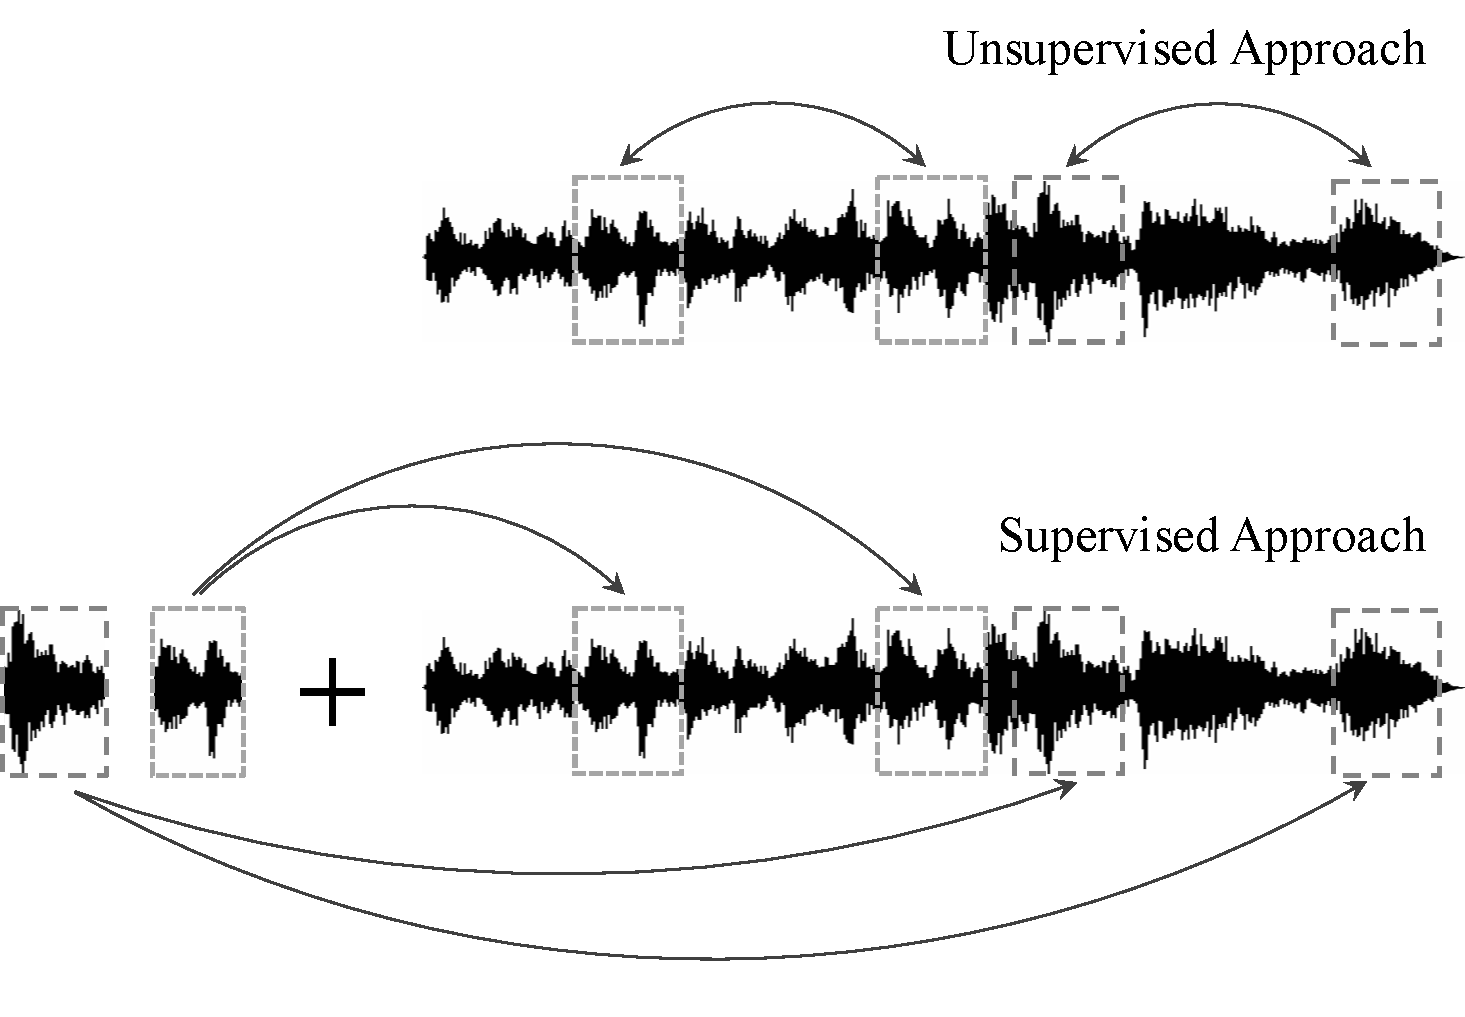
\includegraphics[width=\figSizeEighty]{ch06_patterns/figures/discovery/TwoTypesOfMethodology_BW.pdf}
		\else
			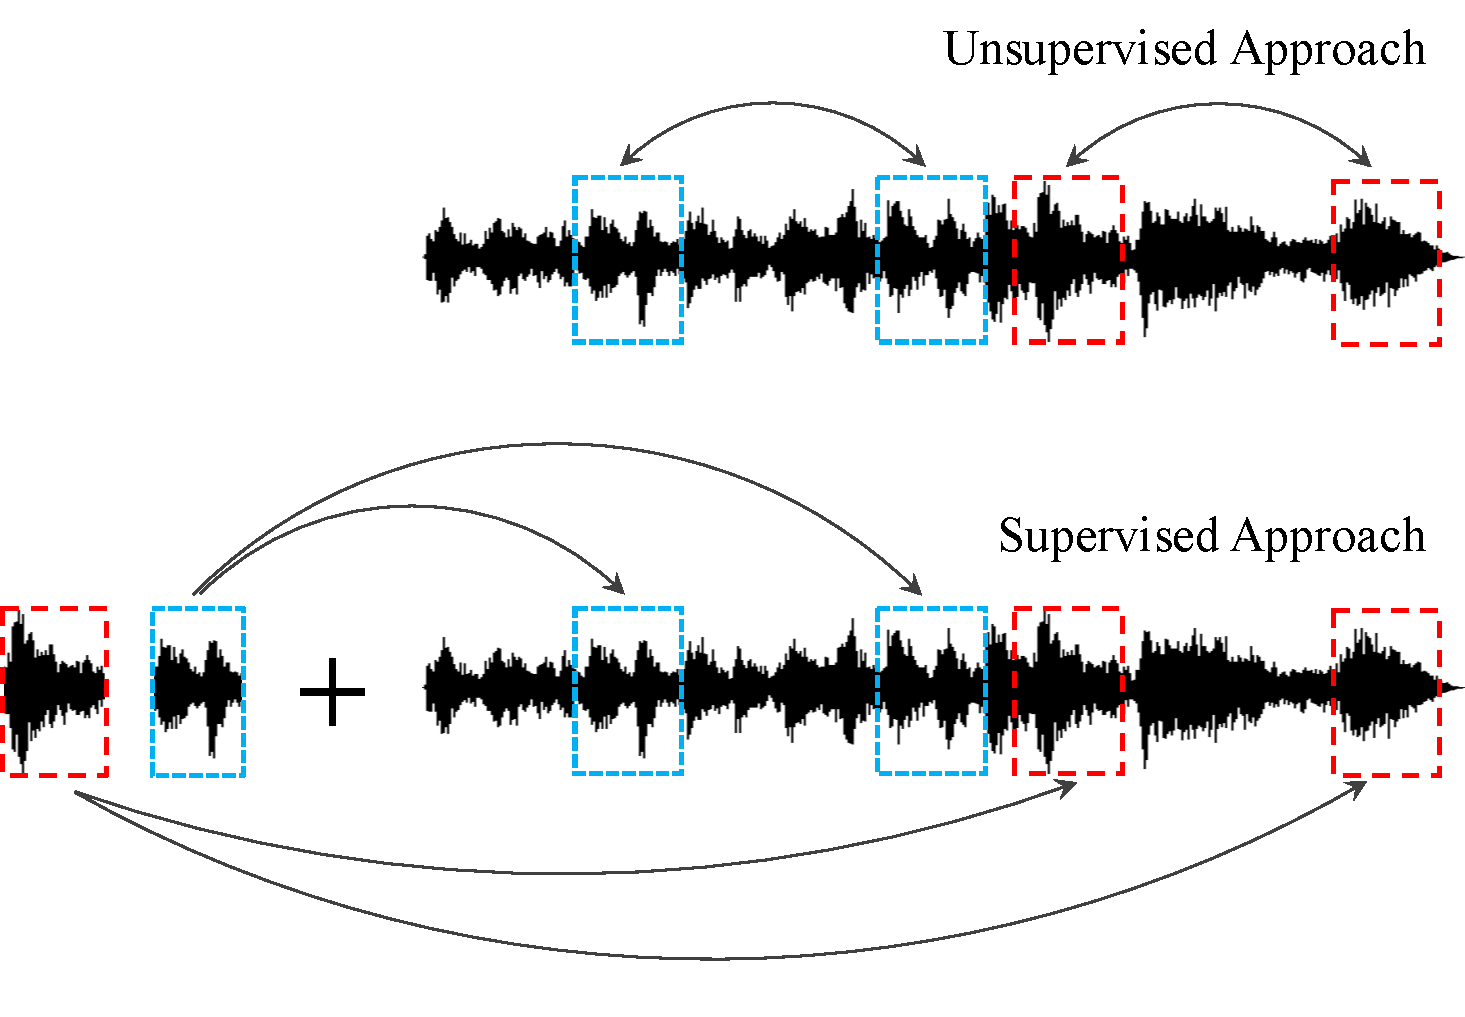
\includegraphics[width=\figSizeEighty]{ch06_patterns/figures/discovery/TwoTypesOfMethodology.pdf}
		\fi
	\end{center}
	\caption{Two types of approaches for pattern extraction in music recordings.}
	\label{fig:types_of_methodologies_for_extraction}
\end{figure}

We identify several caveats in the supervised methodology described above in the context of pattern processing for melodies in \gls{iam}. We believe that using only a supervised methodology severely limits the potential of a pattern-based melodic analysis in \gls{iam}. This is primarily because of the following reasons:

\begin{itemize}
	\item \textbf{Dataset size:} Manually annotating instances of melodic patterns for hundreds of hours of music is a cumbersome process. Since the task of melodic segmentation and similarity is to an extent subjective, ideally speaking, the annotations should be done by multiple domain experts, which makes this task even more challenging. Thus, building a representative and comprehensive corpus of musically meaningful melodic patterns becomes practically unfeasible. This is clearly evident from the size of the datasets used in the existing studies (\secref{sec:sota_pattern_processing_iam}, \tabref{tab:pattern_processing_iam}). The existing datasets typically comprise only a handful of \glspl{raga}, tens of music pieces, tens of unique number of melodic phrases and a single annotator.

	\item \textbf{Knowledge bias:} The process of annotating melodic patterns in audio recordings of \gls{iam} essentially boils down to marking regions in time where a known melodic phrase (\gls{raga} motif, or \gls{mukhda}) occurs. With long audio recordings (some lasting up to an hour) and improvisatory characteristics of this music, annotating every repeated melodic pattern in the melody (using the concept of parallelism) is close to impossible. This can be attributed to the limited memory of human listeners. Thus, an annotated corpus of melodic patterns suffers from a bias (only the patterns known to an annotator are marked), and does not contain all possible repeating patterns. This is also evident from the datasets used in the existing studies (\secref{sec:sota_pattern_processing_iam}, \tabref{tab:pattern_processing_iam}). The annotated melodic patterns either correspond to \gls{mukhda} phrase or to few well known \gls{raga} motifs. 
	
	\item \textbf{Human errors:} We found that even when expert listeners are annotating known melodic phrases they are susceptible to making errors in judgment. One of the possible reasons we discovered is the influence of the local melodic context on phrase segmentation. In one of the pattern datasets, \acrshort{msds} (\secref{sec:corpus_melodic_similarity_dataset}), we found several instances where many repetitions of the melodic patterns were missed by professional musicians. When these missed instances of the patterns were heard in isolation by the same set of musicians, they were correctly identified. The number of the missed pattern instances was significant, nearly 25\% of the total number of annotated patterns. In our conversations with some of these musicians, they commented that the local melodic context masked these patterns and influenced their segmentation. While this phenomenon is yet to be scientifically studied for \gls{iam}, we at least know that melodic pattern annotations done by even professional musicians are prone to such errors. 			
\end{itemize}

One way to circumvent the issues enumerated above is to follow an unsupervised methodology for pattern processing~(\figref{fig:types_of_methodologies_for_extraction}). In such an approach a system discovers patterns in the data without any training examples from an expert or a query pattern. In the context of our work, such a system will not require any examples of the annotated melodic patterns from musicians, and thus can be robust to the issues enumerated above. Also, from our literature review presented in~\secref{sec:sota_pattern_processing_iam}, we notice that there are only a few studies that address the task of discovering short-time melodic patterns in audio music collections. Based on these considerations, in this thesis we follow an unsupervised approach for discovering melodic patterns in sizable audio collections of \gls{iam}. 

The discussion above brings us to an interesting question, what do we mean by a melodic pattern given we do not have any example of it provided by an expert? Recall (\secref{sec:background_terminology}), in the scope of this thesis any recurring melodic fragment is considered as a melodic pattern. We believe that since it repeats, it is not just a coincidence, but it has some significance as the artist rendered the same melodic fragment multiple times. It should be noted that by a recurrence we do not mean a numerical repetition of the pitch sequence. By a recurrence in this context we refer to a musical recurrence of a melodic pattern, which can undergo several melodic variations allowed in the music tradition without loosing its musical identity. In addition, we carefully differentiate the term melodic pattern from melodic motif, wherein the latter is used to refer to a musically significant pattern that is characteristic of a \gls{raga} or a composition (\secref{sec:background_terminology}). 

Along with the aforementioned advantages, there are several challenges in following an unsupervised approach for pattern extraction. One of the most challenging aspects of such approaches is its quantitative evaluation. Due to the absence of ground-truth annotations evaluating such approaches becomes difficult. This becomes even more challenging for a data-driven research methodology since the system parameters are often optimized based on the data. After our first study presented in~\cite{gulati_SITIS_2014} on mining melodic patterns, we realized that selecting optimal values of the system parameters is notoriously difficult in a completely unsupervised setup. As a result, we bootstrap our methodology by first improving one of the core processing blocks in this task, the computation of melodic similarity, within a supervised setup. 

This chapter is divided into four sections, each of which focuses on an important aspect related with pattern processing in \gls{iam}. The contents of these sections are:
\begin{itemize}
	\item In \secref{sec:patterns_evaluation_of_similarity_measures}, we address the task of computing melodic similarity. The main objective is to perform an exhaustive evaluation of different methodologies and parameter settings in order to study their influence on the computation of melodic similarity in \gls{iam}. This section is based on our work presented in~\cite{gulati_ICASSP2015}.
	\item In \secref{sec:patterns_improving_melodic_similarity}, we focus on improving melodic similarity in \gls{iam} by exploiting the culture specific characteristics of the melodies in Carnatic and Hindustani music. This section is based on the study presented in~\cite{gulati_ISMIR_2015}.
	\item In \secref{sec:patterns_melodic_pattern_discovery}, we describe our methodology for discovering melodic patterns in audio music collections of \gls{iam}. This section is largely based on our work presented in~\cite{gulati_SITIS_2014}.
	\item In \secref{sec:patterns_characterization_of_melodic_patterns}, we describe our approach to characterize the discovered melodic patterns in order to identify the ones that correspond to the \gls{raga} motifs. This section is based on our published work in~\cite{gulati_communities_2016}.
\end{itemize}


%################################################################################################################
%########################################### Melodic Similarity Evaluation ######################################
%################################################################################################################


\section{Melodic Similarity: Approaches and Evaluation}
\label{sec:patterns_evaluation_of_similarity_measures}

In this thesis, we regard repeating melodic fragments as melodic patterns. As explained above, the concept of repetition or recurrence in this context is not just a numerical reiteration of exactly the same pitch sequence. But, it is musical in nature, allowing for permitted melodic variations. Thus, the idea of repetition is closely linked to perceptual melodic similarity, which is influenced by several factors including the specificities in a music culture. Our objective in this study is to model this perceptual similarity between short-duration melodic fragments, which will eventually be used for extracting melodic patterns in audio collections of \gls{iam}.

Studying computational models for melodic similarity is particularly interesting in the context of \gls{iam}. This is mainly because this music is inherently improvisatory in nature, and the melodies are largely based around melodic patterns. Due to the melodic improvisation, which is largely governed by \gls{raga} grammar, the surface representation of melodic patterns varies significantly across occurrences. This is specifically true for the characteristic melodic patterns of \glspl{raga} (\secref{sec:melody_in_iam}). These patterns constitute the artists' ground for expressing creativity through improvisation. Hence, even when two melodic patterns are perceptually the same for a musician, their surface melodic representation can be drastically different. To illustrate this, we present an example in~\figref{fig:examples_3_phrases}, where three melodic fragments belonging to the same characteristic \gls{raga} pattern in Hindustani music are shown. We notice that despite these patterns being the occurrences of the same melodic phrase differ considerably in terms of their surface melody representation. In addition to the melodic improvisation, peculiar characteristics of melodies in \gls{iam} such as the usage of \glspl{gamaka} in Carnatic music, the long held steady notes and melodic ornaments in Hindustani music further adds to the complexity of the task.

\begin{figure}
	\begin{center}
		\ifdefined\PRINTVER
			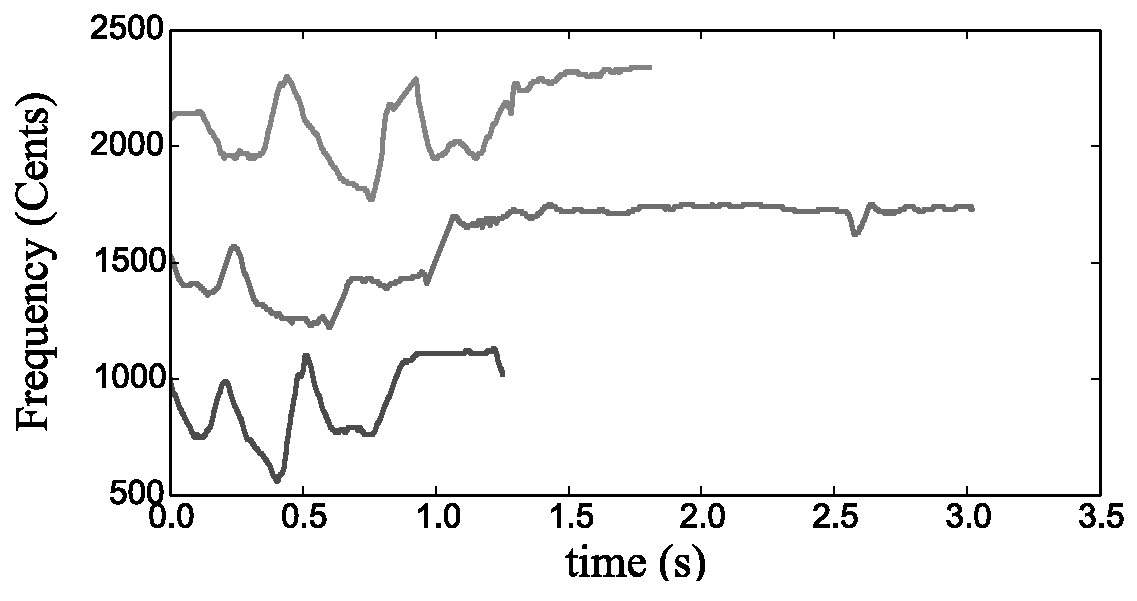
\includegraphics[ width=\figSizeSeventy]{ch06_patterns/figures/SimilarityEvaluation/Hindustani3Patts_BW.pdf}
		\else
			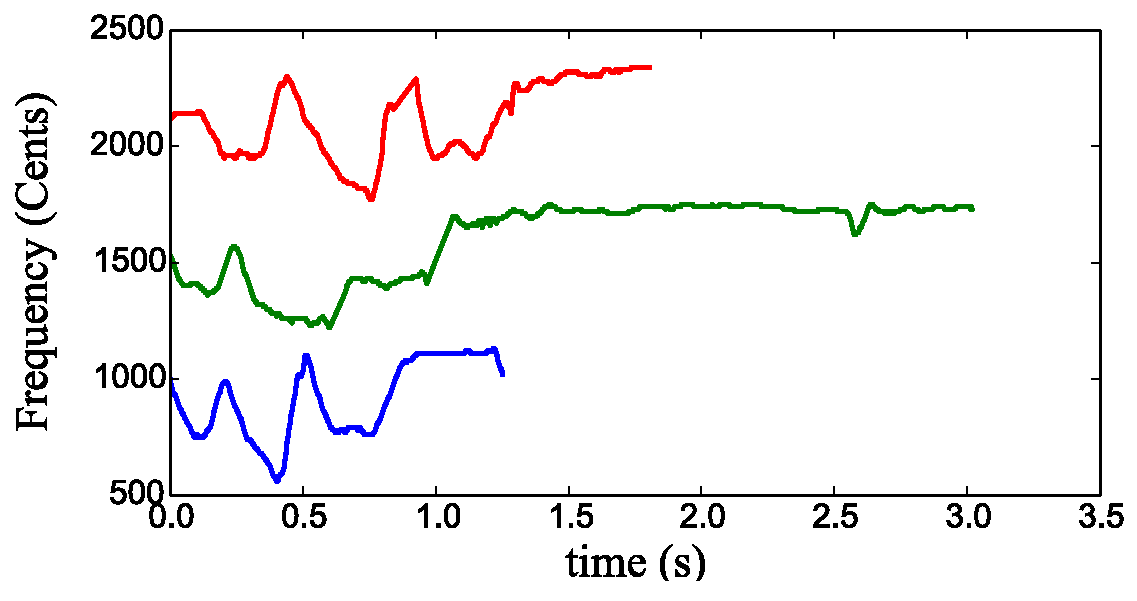
\includegraphics[width=\figSizeSeventyFive]{ch06_patterns/figures/SimilarityEvaluation/Hindustani3Patts.pdf}
		\fi
	\end{center}
	\caption[Examples of difference occurrences of a melodic pattern]{Melodic fragments corresponding to three different renditions of the same characteristic \gls{raga} pattern in Hindustani music. For a better visualization, the patterns are transposed by a frequency offset of 600\,Cents between them.}
	\label{fig:examples_3_phrases}
\end{figure}

Melodic similarity computation is a critical processing block within pattern processing in melodic sequences. In~\secref{sec:sota_pattern_processing_iam} and~\secref{sec:query_by_humming}, we review the existing approaches for melodic pattern processing, which directly or indirectly address the task of melodic similarity. From our review we see that the computational methods to assess melodic similarity have received considerable attention from the \gls{mir} community for a long time. A large number of studies focusing on melodic similarity work with a symbolic representation of music (\secref{sec:motif_in_symbolic_music}). When working with audio music signals, this topic has been studied in depth within the tasks of \acrfull{qbh} and pattern detection in audio recordings (see \secref{sec:query_by_humming} and \secref{sec:sota_pattern_processing_iam}).

The approaches proposed for computing melodic similarity primarily differ in the choices made for the main processing steps comprising: melody representation, melody segmentation, pitch transposition invariance, tempo or timing invariance, and distance measure (\secref{sec:query_by_humming}). In addition, every method has a set of additional choices for selecting the optimal parameters at each processing step. Since the melodic characteristics across music traditions vary considerably, these procedures and parameter choices cannot be generalized to all music traditions. Therefore, studies that perform a comparative evaluation of different methods and analyse the effect of different parameter settings for a specific type of music material are valuable to the community~\citep{dannenberg2007comparative,Rao2014,XavierSerra2011}.

During the course of this thesis work several approaches have been proposed for computing melodic similarity in \gls{iam} (\secref{sec:sota_pattern_processing_iam}). However, a consensus on the best approach has yet not been reached. This is mainly because these approaches are evaluated using different datasets and under different experimental setup. To the best of our knowledge there has not been any study that systematically evaluates the influence of different choices of procedures and parameter values involved in similarity computation in melodies of \gls{iam}.



%In the literature (Section XX) there are a number of approaches proposed for computing melodic similarity\TODO{refs}. These approaches vary depending upon the melodic characteristics of a music tradition, duration of the melodic fragment and the task under study. There are a number of parameters and processing steps involved in the computation of melodic similarity such as the choice of melodic representation, frequency normalization and the distance measure. For music traditions such as XXX YYY kind of melodic representations are frequently used. some state of the art explanation.\TODO{This paragraph will be finished after literature review.}

%As seen in the literature review that a number of successful strategies for computing melodic similarity work on transcribed melodic representation\TODO{ref}. For \gls{iam}, where one of the characteristic aspects of melodies is its gliding transitory movement, transcription becomes a complex and an ill-defined task\TODO{ref}. Melodic representation directly influences the choice of an optimal distance measure. Therefore, due to all these factors there is need to comprehensively assess the influence of different system parameters and procedures on the accuracy of melodic similarity for \gls{iam}. 

%We study modeling of melodic similarity by casting it as a retrieval task. For this we use collections of audio recordings for which occurrences of characteristic melodic phrases of different \glspl{raga} are annotated by professional musicians~(\secref{sec:corpus_melodic_similarity_dataset}). We consider all the occurrences of a characteristic melodic phrase melodically more similar to each other than any random melodic fragment extracted from the collection. Thus, if we consider a characteristic melodic phrase as a query and compute melodic similarity with every possible melodic fragment in the collection, we expect all other occurrences of this characteristic phrase to appear on the top of the search results. Note that working with characteristic melodic phrases of \glspl{raga} for developing melodic similarity models adds to the complexity of the task. This is because while our system computes melodic similarity by comparing two melodic fragments, musician's have annotated these phrases by segmenting and identifying them individually. Characteristic melodic phrases of \glspl{raga} are distinctly recognizable by musicians and therefore annotating them do not involve any comparison of two melodic fragments. 

% In this section we address this issue by performing an exhaustive evaluation of several methodologies and parameter settings for computing similarity between short-time melodic patterns in \gls{iam}.


In this section, we describe a string matching-based approach for computing similarity between two short-time melodic patterns in \gls{iam}. Our objective is to perform a comprehensive evaluation of different variants of this approach to study the influence of different system parameters and procedures on melodic similarity for \gls{iam}. We evaluate 560 variants put together by combining different choices of the sampling rate of the melody representation, pitch quantization levels, melody normalization techniques, uniform time-scaling and distance measures. We believe the findings of this study will pave the way for developing unsupervised melodic pattern discovery approaches as described in the subsequent sections, whose evaluation is a challenging and, many times, ill-defined task. The current section is based on our published work presented in~\cite{gulati_ICASSP2015}.

\subsection{Method}
\label{sec:method_similarity_evaluation}


\begin{figure}
	\begin{center}
		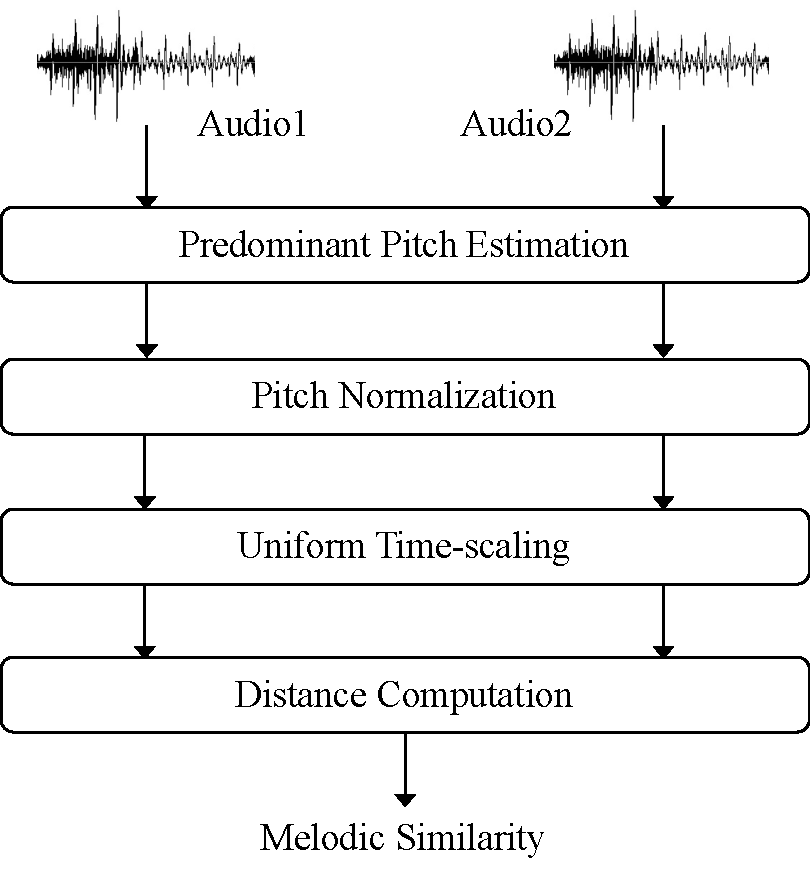
\includegraphics[width=\figSizeSixty]{ch06_patterns/figures/SimilarityEvaluation/melodic_similarity_blockd.pdf}
	\end{center}
	\caption[Block diagram for computing melodic similarity]{Block diagram of the methodology followed for computing melodic similarity from audio recordings.}
	\label{fig:block_diagram_melodic_similarity}
\end{figure}

The block diagram for computing melodic similarity is shown in~\figref{fig:block_diagram_melodic_similarity}. There are four main processing blocks involved in this task: predominant pitch estimation, pitch normalization, uniform time-scaling, and distance computation. We explore different combinations of the choices made for the processing steps and the parameter settings.

\subsubsection{Predominant Pitch Estimation}
\label{sec:patterns_melodic_similarity_representation}

We follow common practice and represent melody by the predominant pitch of an audio signal. For Carnatic music, we use a state-of-the-art melody extraction method proposed by~\cite{Salamon2012} as described in~\secref{sec:data_preprocessing_predominant_melody_estimation}. We use a frame size of 46\,ms and a hop size of 5\,ms. We do not perform any post-processing on the pitch contours except for interpolating short unvoiced segments (\secref{sec:data_processing_pitch_interpolation}). For Hindustani music we use semi-automatically extracted predominant pitch contours included in the dataset that we use to perform evaluations (\secref{sec:corpus_melodic_similarity_dataset}). This dataset along with these pitch contours have been used in several studies on similar topics~\citep{Rao2014,Ross2012b,Ross2012}. This eases the comparison of results across studies and also avoids the effect of pitch errors often present in fully automated melody extraction algorithms. We convert the pitch values from Hertz to Cents in order to make the representation musically more relevant (\secref{sec:data_processing_cent_conversion}).

Since automatic assessment of melodic similarity is a computationally expensive task, particularly when done on large audio archives, we desire the minimum possible sampling rate of the melody without compromising the accuracy. We therefore analyse the effect of different sampling rates of the melody representation on melodic similarity. We consider 5 sampling rates 100, 67, 50, 40 and 33\,Hz of predominant pitch, implemented by down-sampling the original melody sequence as described in~\secref{sec:data_processing_pitch_resampling}. We denote these parameter settings by $\sRate_{100}, \sRate_{67}, \sRate_{50}, \sRate_{40}$ and $\sRate_{33}$. Note that in our literature review we found that none of the existing approaches performed a systematic evaluation of this important parameter for melodies in \gls{iam}~(\secref{sec:sota_pattern_processing_iam}).

\subsubsection{Pitch Normalization}
\label{sec:patterns_melodic_similarity_transposition_invariance}

The absolute values of the pitch samples (in both Hertz and Cent scale) corresponding to different occurrences of a melodic pattern may differ across artists and even within the same recording. There are two main reasons for this. First, in \gls{iam} the reference frequency for a melody rendition is the tonic of the lead artist (\secref{sec:melody_in_iam}), which typically varies across artists. And second, a melodic pattern may recur in a different octave within the same recording. Therefore, a meaningful comparison of the melodic patterns across different artists and across different sections of a recording is possible only when the similarity computation is invariant to pitch transpositions. Out of these two cases, the latter is relatively infrequent, and is ignored in most of the existing studies (\secref{sec:sota_pattern_processing_iam}).

We experiment with five different normalization techniques to achieve pitch transposition invariance. They are as follows.

\begin{enumerate}
	\item Normalizing the pitch values of a melodic pattern by the tonic of the lead artist of the recording ($\mNorm_{\mathrm{tonic}}$). This is implemented by considering the tonic frequency of the lead artist as the base frequency in Hertz to Cents conversion (see~\secref{sec:tonic_normalization})

	\item Zero mean normalization ($\mNorm_{\mathrm{mean}}$), where mean of the melodic pattern is subtracted from each pitch sample so that the resulting mean of the pattern becomes zero
	
	\item Zero median normalization ($\mNorm_{\mathrm{median}}$), where median of the melodic pattern is subtracted from each pitch sample so that the resulting median of the pattern becomes zero
	\item Z-normalization ($\mNorm_{\mathrm{Z}}$), where from each pitch sample we subtract the mean of the melodic pattern and subsequently divide it by the standard deviation of the pattern
	\item Median absolute deviation normalization ($\mNorm_{\mathrm{MAD}}$), where from each pitch sample we subtract the median of the melodic pattern and subsequently divide it by the median absolute deviation of the pattern
\end{enumerate}

In the case of $\mNorm_{\mathrm{tonic}}$ the tonic pitch of the lead artist is identified using \acrshort{tonicid_justin} method, the best performing method resulted from our exhaustive evaluations~(\secref{sec:pre_processing_tonic_identification_summary}). Furthermore, since the reference frequency of the melody is known for this case ($\mNorm_{\mathrm{tonic}}$), the pitch values can be quantized, as reported in other studies~\citep{Ross2012b}. Hence, we additionally experiment with two quantization levels: semitone level, quantizing pitch values to 100\,Cents interval ($\mNorm_{\mathrm{tonicQ12}}$) and quarter-tone level, quantizing pitch values to 50\,Cents interval ($\mNorm_{\mathrm{tonicQ24}}$). Note that the tonic normalization ($\mNorm_{\mathrm{tonic}}$) is helpful only in the scenarios where the frequency transpositions are due to the different tonic frequencies of the lead artists across recordings. It does not handle the cases where a pattern recurs in a different octave or a tetra-chord within the same recording. In total, we consider 8 different normalization variants, including the one without any normalization ($\mNorm_{\mathrm{off}}$). 


\subsubsection{Uniform Time-scaling}
\label{sec:patterns_melodic_similarity_time_scaling}

In order to compensate for global tempo variations across occurrences of a melodic pattern, a typical approach is to consider multiple uniformly time-scaled versions of the patterns~\citep{mazzoni2001melody,zhu2003query,kotsifakos2012survey}. Such tempo differences if not handled can significantly degrade the performance in retrieval scenarios where fixed duration patterns are considered. We experiment with two possibilities: first, we do not apply any time-scaling to the patterns ($\uTScaling_{\mathrm{off}}$) and second, we generate 5 copies of every pattern before similarity computation by uniformly time-scaling it by a factor of 0.9, 0.95, 1, 1.05 and 1.1 ($\uTScaling_{\mathrm{on}}$). We implement uniform time-scaling using cubic interpolation. 


\subsubsection{Distance Computation}
\label{sec:patterns_melodic_similarity_dissimilarity measures}

To measure the melodic similarity between two patterns we consider two categories of commonly used distance measures (see \secref{sec:sota_pattern_processing_iam} and \secref{sec:query_by_humming}): Euclidean distance ($\distPattMeasure_{\mathrm{Euc}}$) and \acrfull{dtw}-based distance. Euclidean distance is a non-parametric distance measure (\secref{sec:euclidean_distance}, \eqnref{eq:euclidean_distance}), whereas, \gls{dtw}-based distance measure has many variants and parameters to select. 

In this study we consider the whole sequence matching \gls{dtw} variant and two possibilities of the local constraint~(\secref{sec_DTW_distance_measure}):

\begin{itemize}
	\item Where the \gls{dtw} step condition is $\lbrace(1,1), (1,1), (1,1)\rbrace$, which is without any local constraint. We denote this variant by~$\distPattMeasure_{\mathrm{DTW\_L0}}$. In this variant the \gls{dtw} accumulated cost matrix is computed using~\eqnref{eq:dtw_classic_cost_matrix_computation}.
	\item Where the \gls{dtw} step condition is $\lbrace(2,1), (1,1), (1,2)\rbrace$, which is with a local constraint We denote this variant by~$\distPattMeasure_{\mathrm{DTW\_L1}}$. In this variant the \gls{dtw} accumulated cost matrix is computed using~\eqnref{eq:dtw_local_constraint_cost_matrix_computation}.
\end{itemize}

In addition, for both these \gls{dtw} variants we also apply Sakoe-Chiba global band constraint~\citep{Sakoe78TASLP} with the width of the band as 5\%, 10\% and 90\% of the pattern length. Note that 90\% band width in the global constraint is to simulate the case of unconstrained \gls{dtw}. We denote these combinations by $\distPattMeasure_{\mathrm{DTW\_L0\_G5}}$, $\distPattMeasure_{\mathrm{DTW\_L0\_G10}}$, $\distPattMeasure_{\mathrm{DTW\_L0\_G90}}$, $\distPattMeasure_{\mathrm{DTW\_L1\_G5}}$, $\distPattMeasure_{\mathrm{DTW\_L1\_G10}}$, and $\distPattMeasure_{\mathrm{DTW\_L1\_G90}}$, respectively. In total, we consider 7 variants of distance measures for melodic similarity computation.

%
%In this study we consider the whole sequence matching \gls{dtw} variant and two possibilities of the local constraints: first, without any local constraint ($\distPattMeasure_{\mathrm{DTW\_L0}}$), where the \gls{dtw} step condition is $\lbrace(1,1), (1,1), (1,1)\rbrace$, and second, with local constraint ($\distPattMeasure_{\mathrm{DTW\_L1}}$), where $\lbrace(2,1), (1,1), (1,2)\rbrace$ is the \gls{dtw} step condition (see \secref{sec_DTW_distance_measure}). In addition, for both these \gls{dtw} variants we also apply Sakoe-Chiba global band constraint~\cite{Sakoe78TASLP} with the width of the band as 5\%, 10\% and 90\% of the pattern length. Note that 90\% band width in the global constraint is to simulate the case of unconstrained \gls{dtw}. We denote these combinations by $\distPattMeasure_{\mathrm{DTW\_L0\_G5}}$, $\distPattMeasure_{\mathrm{DTW\_L0\_G10}}$, $\distPattMeasure_{\mathrm{DTW\_L0\_G90}}$, $\distPattMeasure_{\mathrm{DTW\_L1\_G5}}$, $\distPattMeasure_{\mathrm{DTW\_L1\_G10}}$, and $\distPattMeasure_{\mathrm{DTW\_L1\_G90}}$, respectively. In total, we consider 7 variants of distance measures for melodic similarity computation.

Since the length of the melodic patterns are different, before computing similarity between two patterns we apply a uniform time-scaling to make their lengths equal. We select the maximum of the lengths of the two patterns as the final length. This operation is a must for the Euclidean distance and has been shown to have a slightly beneficial effect for \gls{dtw}~\citep{Ratanamahatana2004,zhu2003query}.


\subsection{Evaluation Methodology}
\label{sec:patterns_melodic_similarity_evaluation_methodology}

We use \acrshort{msds} dataset for evaluating different variants of the method for computing melodic similarity (\secref{sec:corpus_melodic_similarity_dataset}). Since melodic characteristics across Carnatic and Hindustani music differ considerably, \acrshort{msds} comprises two sub-datasets, \acrshort{msds_iitm_cmd} and \acrshort{msds_iitb_hmd}. For evaluation of melodic similarity in Carnatic music we use \acrshort{msds_iitm_cmd} dataset, and in Hindustani music we use \acrshort{msds_iitb_hmd} dataset. Both these datasets contain annotations comprising occurrences of five different characteristic phrases of the \glspl{raga}~(\tabref{tab:categorywise_details_melodic_similarity_dataset}). Note that we regard each characteristic phrase as one type of a pattern.

We consider every annotated pattern as a query and perform an exhaustive search in the target search space comprising all the annotated patterns in the entire music collection. To make the experimental setup closer to the real world scenario, we add melodic segments other than the annotated patterns in the target search space, which act as noise (referred to as noise candidates). We generate these candidates by randomly selecting short fragments of the melodies from the dataset. The time stamps of the starting of these noise candidates are generated using a uniform distribution, and the lengths are determined using the distribution of the duration values of the annotated patterns. The total number of noise candidates added is 100 times the number of annotated patterns for each dataset. For every query, we order the search results by the similarity values and consider the top 1000 nearest neighbors for evaluation. A retrieved pattern is considered as a true hit only if it belongs to the same pattern type as the query pattern. 

In the experimental setup described above, the segmentation of the melodic patterns is done using the ground-truth annotations. However, in several tasks such as in melodic pattern discovery the segmentation information might not be present. Thus, to simulate a retrieval scenario where the pattern boundaries are not known \textit{a priori}, we also consider a simple extension to the experiment by assuming the target pattern length to be equal to the length of the query pattern. We perform all our experiments for both these setups. 

We evaluate all possible combinations of the choices made at each step of the melodic similarity computation discussed in~\secref{sec:method_similarity_evaluation}. We consider 5 different sampling rates of the melody representation, 8 different normalization scenarios, 2 possibilities of uniform time-scaling and 7 variants of the distance measures. In total, we evaluate 560 different variants.

To quantify the performance of a melodic similarity variant considered in this study we use \acrfull{map}, a typical evaluation measure in information retrieval~\citep{manning2008introduction}. \Gls{map} is computed by taking the mean of the average precision values of each query in the dataset. This way, we have a single number to evaluate and compare the performance of a variant. In order to assess if the difference in the performance of any two variants is statistically significant, we use the Wilcoxon signed rank-test~\citep{wilcoxon1945individual} with $\pVal < 0.01$. To compensate for multiple comparisons, we apply the Holm-Bonferroni method~\citep{holm1979simple}. Thus, considering that we compare 560 different variants, we effectively use a much more stringent criterion than $\pVal < 0.01$ for measuring statistical significance.


\subsection{Results and Discussion}
\label{sec:patterns_melodic_similarity_results_discussions}


\begin{table} 
	\begin{centering}
	\tabcolsep = 0.12cm
	\begin{tabular}{ c | c c c c c}
\tabletop
		Dataset   	& 	\acrshort{map}	&	Srate		&	Norm 	&	TScale 		&	Dist \\	
\tablemid
		\multirow{3}{*}{\acrshort{msds_iitm_cmd}}   	
		& 	0.413 	&	$\sRate_{67}$			&	$\mNorm_{\mathrm{mean}}$ 	&	$\uTScaling_{\mathrm{off}}$		&	$\distPattMeasure_{\mathrm{DTW\_L1\_G90}}$\\	
		& 	0.412 	&	$\sRate_{67}$		&	$\mNorm_{\mathrm{mean}}$ 	&	$\uTScaling_{\mathrm{on}}$		&	$\distPattMeasure_{\mathrm{DTW\_L1\_G10}}$\\	
		& 	0.411	&	$\sRate_{100}$		&	$\mNorm_{\mathrm{mean}}$ 	&	$\uTScaling_{\mathrm{off}}$		&	$\distPattMeasure_{\mathrm{DTW\_L1\_G90}}$\\	
		\hline		
		\multirow{3}{*}{\acrshort{msds_iitb_hmd}}   	
		& 	0.552	&	$\sRate_{100}$		&	$\mNorm_{\mathrm{tonic}}$ 	&	$\uTScaling_{\mathrm{off}}$		&	$\distPattMeasure_{\mathrm{DTW\_L0\_G90}}$\\	
		& 	0.551 	&	$\sRate_{67}$	&	$\mNorm_{\mathrm{tonic}}$ 	&	$\uTScaling_{\mathrm{off}}$		&	$\distPattMeasure_{\mathrm{DTW\_L0\_G90}}$\\	
		& 	0.547 	&	$\sRate_{50}$		&	$\mNorm_{\mathrm{tonic}}$ 	&	$\uTScaling_{\mathrm{off}}$		&	$\distPattMeasure_{\mathrm{DTW\_L0\_G90}}$\\	
\tablebot		
	\end{tabular}
	\caption[\acrshort{map} scores and parameter details for the three best performing variants of the method for computing melodic similarity]{\acrshort{map} score and the details of parameter settings for the three best performing variants for \acrshort{msds_iitm_cmd} and \acrshort{msds_iitb_hmd}. Srate: sampling rate of the melody representation, Norm: normalization technique, TScale: uniform time-scaling and Dist: distance measure.}
	\label{tab:melodic_similarity_results}
\par \end{centering}	
\end{table}


In this section we present the results of our evaluation of the 560 variants for each of the datasets, \acrshort{msds_iitm_cmd} and \acrshort{msds_iitb_hmd}. We order the variants in the decreasing order of their \gls{map} scores and present only the three best performing variants in~\tabref{tab:melodic_similarity_results}. For complete results see the companion page for this study (\appref{app:mypapers}).

In Table~\ref{tab:melodic_similarity_results} (top half), we show the \gls{map} scores and the details of parameter settings for \acrshort{msds_iitm_cmd} dataset. We see that the best performing variant has a \gls{map} score of 0.413. Having a look at the whole list, we observe that for \acrshort{msds_iitm_cmd}, in the ranked list of the 560 variants, top performing variants consistently use higher sampling rates (either $\sRate_{100}$, or $\sRate_{67}$). This can be attributed to the rapid oscillatory melodic movements present in Carnatic music, whose preservation requires a higher sampling rate. The top variants invariably use the zero mean normalization ($\mNorm_{\mathrm{mean}}$), suggesting that there are several repeated instances of the melodic patterns that are pitch transposed within the same recording. In addition, top variants also use \gls{dtw}-based distance with local constraint (either $\distPattMeasure_{\mathrm{DTW\_L1\_G10}}$ or $\distPattMeasure_{\mathrm{DTW\_L1\_G90}}$), indicating that melodic fragments are prone to large pathological warping that can significantly degrade the performance. We do not observe any consistency in the usage of uniform time-scaling. However, it strongly correlates with the global constraint in the \gls{dtw} distance. In majority of the top ranked variants, $\uTScaling_{\mathrm{on}}$ consistently occurs with $\distPattMeasure_{\mathrm{DTW\_L1\_G10}}$, and $\uTScaling_{\mathrm{off}}$ consistently occurs with $\distPattMeasure_{\mathrm{DTW\_L1\_G90}}$. This suggests that a combination of uniform time-scaling and narrow global band constrained variant of \gls{dtw} is able to handle the same degree of non-linear timing variations as can be handled by a globally unconstrained \gls{dtw}. However, the former configuration is computationally more efficient than the latter. We also performed an analysis of several (small distance) false positives and found that the \gls{map} scores for a number of queries were low because of the spurious errors in the predominant pitch.


The \gls{map} scores and the details of parameter settings for \acrshort{msds_iitb_hmd} dataset are shown in~\tabref{tab:melodic_similarity_results} (bottom half). Compared to \acrshort{msds_iitm_cmd}, the best \gls{map} score for \acrshort{msds_iitb_hmd} is higher (0.55). Amongst the top ranked variants there is no consensus on the sampling rate of the melody representation. All the top ranked variants have the same parameter values except the sampling rate. This suggests that the sampling rates considered in this study have no significant effect on the melodic similarity for \acrshort{msds_iitb_hmd}. This can be attributed to the fact that the recordings in \acrshort{msds_iitb_hmd} are slow-medium tempo music pieces that do not have fast oscillatory melodic movements, as was the case with \acrshort{msds_iitm_cmd}. Furthermore, for \acrshort{msds_iitb_hmd}, we observe that the variants using $\mNorm_{\mathrm{tonic}}$, $\mNorm_{\mathrm{tonicQ12}}$ or $\mNorm_{\mathrm{tonicQ24}}$ perform better than the ones using $\mNorm_{\mathrm{mean}}$, which is in contrast to the observation for \acrshort{msds_iitm_cmd}. This is primarily because in Carnatic music in our datasets there are many cases where a pattern recurs in a different octave within the same recording, whereas, in Hindustani music, such cases are rare. In general, we see that the \gls{dtw}-based distance performs better than the euclidean distance, and the \gls{dtw} variant without a global constraint ($\distPattMeasure_{\mathrm{DTW\_L1\_G90}}$ or $\distPattMeasure_{\mathrm{DTW\_L0\_G90}}$) is preferred. This implies that the repeated instances of melodic patterns in \gls{iam} (specifically in Hindustani music) have large non linear timing variations.

\begin{figure}[h]
	\begin{center}
		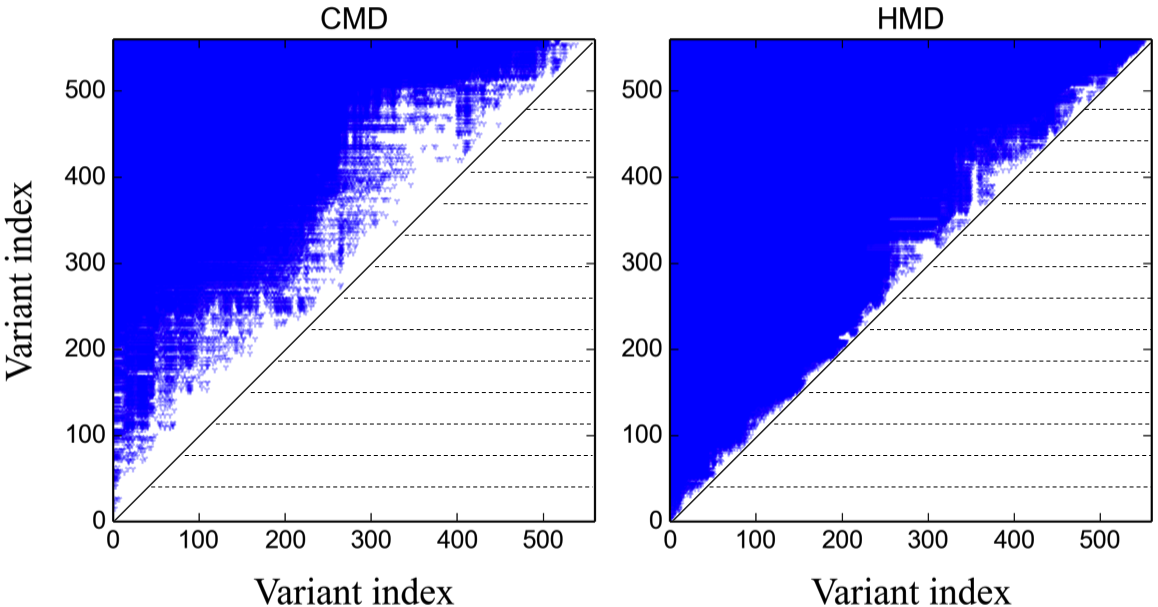
\includegraphics[width=\figSizeNinety]{ch06_patterns/figures/SimilarityEvaluation/StatisticalDiff.png}
	\end{center}
	\caption[Matrix indicating the statistical significance of the performance difference between different method variants]{Matrix indicating the statistical significance of the performance difference between every variant pair for \acrshort{msds_iitm_cmd} and \acrshort{msds_iitb_hmd}. Variant pairs, where the difference in the performance is statistically significant, are marked by blue dots. Only the superscript in the name of the dataset is used in the figure title.}
	\label{fig:patterns_statistical_significance_similarity_evaluation}
\end{figure}

To assess the statistical significance of the results we compare every possible pair of the variants ($^{560}C_{2}$ = 156520 comparisons). The results are shown in~\figref{fig:patterns_statistical_significance_similarity_evaluation}, where both the axes are the index of the variants in the ranked list. For every variant pair with index $i$ and $j$, we mark the pixel~($i$,$j$) if the difference is statistically significant. From~\figref{fig:patterns_statistical_significance_similarity_evaluation} we see that a majority of variant pairs have a statistically significant difference in the \gls{map} scores. This indicates that the task of computing melodic similarity is sensitive to the choice of parameters and processing steps, and a small change in the choices made in a variant can lead to a significantly different \gls{map} score. Furthermore, as the marked pixels are higher in number for \acrshort{msds_iitb_hmd}, this sensitivity is even higher for \acrshort{msds_iitb_hmd} compared to \acrshort{msds_iitm_cmd}.


\begin{figure}
	\begin{center}
		\ifdefined\PRINTVER
			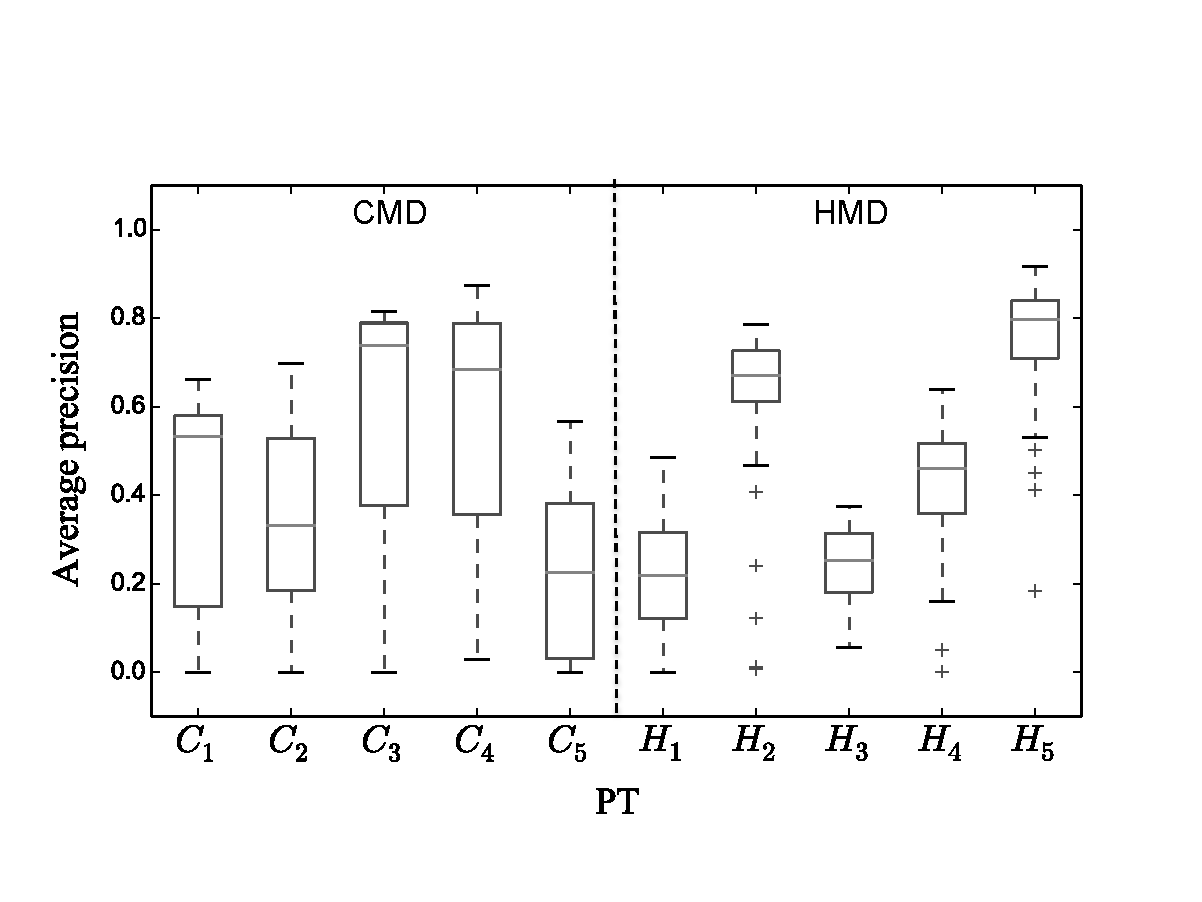
\includegraphics[width=\figSizeEightyFive]{ch06_patterns/figures/SimilarityEvaluation/CMD_HMD_CW_MAP_BW.pdf}
		\else
			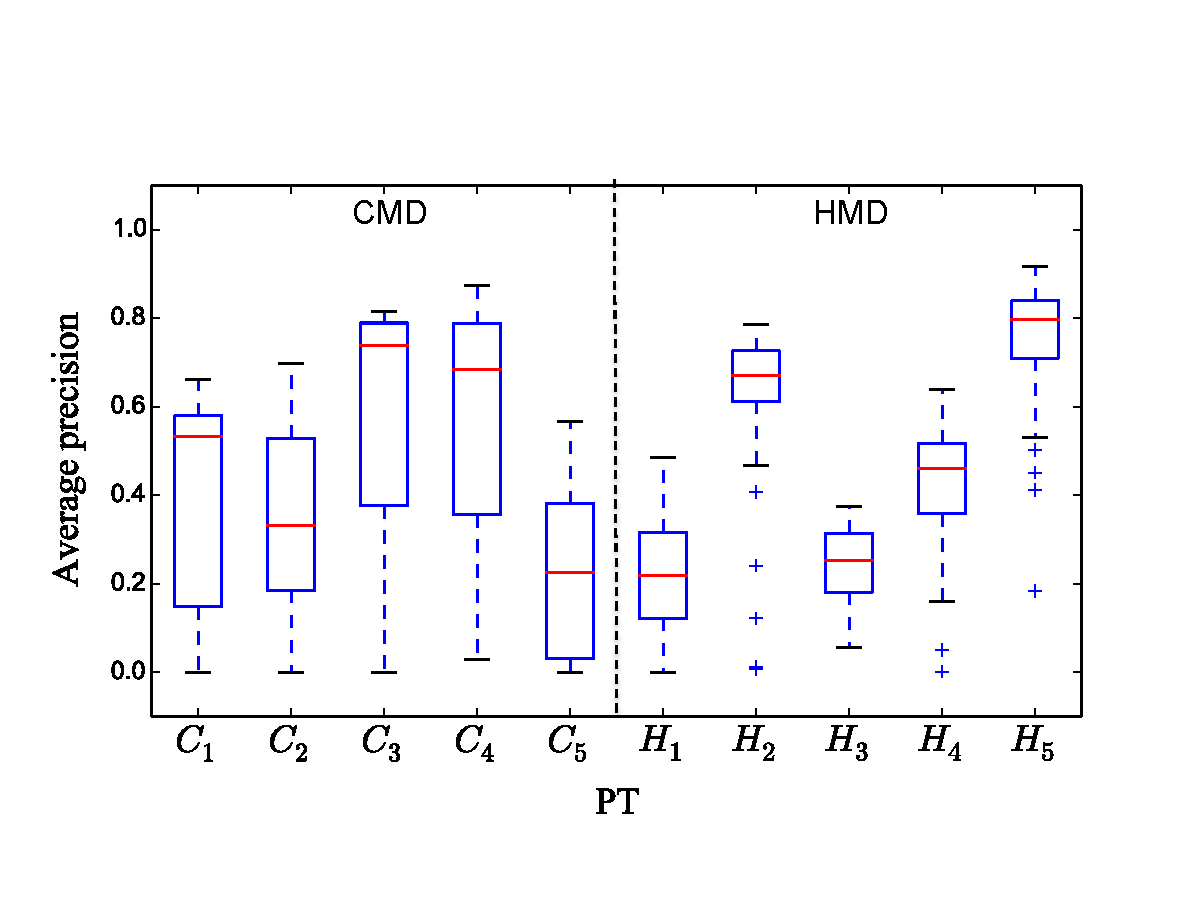
\includegraphics[width=\figSizeEightyFive]{ch06_patterns/figures/SimilarityEvaluation/CMD_HMD_CW_MAP.pdf}
		\fi
	\end{center}
	\caption[Boxplot of average precision values for different types of melodic patterns]{Boxplot of the average precision values for each pattern type~(PT) in \acrshort{msds_iitm_cmd} and \acrshort{msds_iitb_hmd}. Only the superscript in the name of the dataset is used for labeling.}
	\label{fig:patterns_similarity_evaluation_results_boxplot}
\end{figure}


To analyse the consistency in the performance across pattern types, we present the boxplot of the average precision values for each pattern type in~\figref{fig:patterns_similarity_evaluation_results_boxplot}. For this, we consider only the top performing variant for each dataset. We see that the \gls{map} scores vary considerably across pattern types for both \acrshort{msds_iitm_cmd} and \acrshort{msds_iitb_hmd}. Furthermore, we observe that the intra pattern type variance of the \gls{map} scores is higher for \acrshort{msds_iitm_cmd} as compared to \acrshort{msds_iitb_hmd}. In addition, we observe that the pattern types $H_2$ and $H_5$ have a higher \gls{map} value compared to other pattern types in \acrshort{msds_iitb_hmd}. Interestingly, $H_2$ and $H_5$ are also the pattern types for which variance in the length is lower and number of occurrences is higher than others in \acrshort{msds_iitb_hmd} (\tabref{tab:categorywise_details_melodic_similarity_dataset}). This correlation is not evident in \acrshort{msds_iitm_cmd}.
%\COMMENT{there has to be a musical explanation here, whats happening? Ask Kaustuv and Vignesh}


\begin{table} 
	\begin{centering}
		\tabcolsep = 0.12cm
		\begin{tabular}{ c | c c c c c}
			\tabletop
			Dataset   	& 	\acrshort{map}	&	Srate		&	Norm 	&	TScale 		&	Dist \\	
			\tablemid
			\multirow{3}{*}{\acrshort{msds_iitm_cmd}}   	
			& 	0.279 	&	$\sRate_{67}$		&	$\mNorm_{\mathrm{mean}}$ 	&	$\uTScaling_{\mathrm{on}}$		&	$\distPattMeasure_{\mathrm{DTW\_L1\_G10}}$\\	
			& 	0.277 	&	$\sRate_{67}$		&	$\mNorm_{\mathrm{tonicQ12}}$ 	&	$\uTScaling_{\mathrm{on}}$		&	$\distPattMeasure_{\mathrm{DTW\_L1\_G10}}$\\	
			& 	0.275	&	$\sRate_{100}$		&	$\mNorm_{\mathrm{tonicQ12}}$ 	&	$\uTScaling_{\mathrm{on}}$		&	$\distPattMeasure_{\mathrm{DTW\_L1\_G10}}$\\	
\tablemid
			\multirow{3}{*}{\acrshort{msds_iitb_hmd}}   	
			& 	0.259	&	$\sRate_{40}$		&	$\mNorm_{\mathrm{tonicQ12}}$ 	&	$\uTScaling_{\mathrm{on}}$		&	$\distPattMeasure_{\mathrm{DTW\_L1\_G90}}$\\	
			& 	0.259 	&	$\sRate_{100}$		&	$\mNorm_{\mathrm{tonicQ12}}$ 	&	$\uTScaling_{\mathrm{on}}$		&	$\distPattMeasure_{\mathrm{DTW\_L1\_G90}}$\\	
			& 	0.259 	&	$\sRate_{67}$		&	$\mNorm_{\mathrm{tonicQ12}}$ 	&	$\uTScaling_{\mathrm{on}}$		&	$\distPattMeasure_{\mathrm{DTW\_L1\_G90}}$\\	
			\tablebot		
		\end{tabular}
		\caption[\acrshort{map} scores and parameter details for the three best performing variants of the method for computing melodic similarity, without using ground-truth segmentation]{\acrshort{map} score and the details of parameter settings for the three best performing variants for \acrshort{msds_iitm_cmd} and \acrshort{msds_iitb_hmd} dataset. These results are corresponding to the experiment where target patterns' length is not read from the ground-truth annotations but is considered to be same as the query pattern length. Srate: sampling rate of the melody representation, Norm: normalization technique, TScale: uniform time-scaling and Dist: distance measure.}
		\label{tab:melodic_similarity_results_var2}
\par \end{centering}		
\end{table}

So far we have seen the results in the experimental setup where the melodic patterns are segmented using the ground-truth annotations. We now present the results corresponding to the other experimental setup described in~\secref{sec:patterns_melodic_similarity_evaluation_methodology}, where the target pattern lengths are considered to be the same as that of the query pattern. We evaluate all 560 variants of the method as done above on both the datasets under this experimental setup. In~\tabref{tab:melodic_similarity_results_var2} we show the \gls{map} scores of the top performing variants for both the datasets \acrshort{msds_iitm_cmd} and \acrshort{msds_iitb_hmd}. We find that the \gls{map} score for the best performing variant decreases from 0.41 to 0.28 and 0.55 to 0.26 for \acrshort{msds_iitm_cmd} and \acrshort{msds_iitb_hmd}, respectively. This indicates that the melodic similarity computation task becomes much more challenging in the absence of an accurate melodic segmentation method. For this experimental setup the trend in the sampling rate for Carnatic and Hindustani music remain the same as we saw in~\tabref{tab:melodic_similarity_results}, which is that a higher sampling rate is desired for representing melodic patterns in Carnatic music. In terms of the normalization we see that surprisingly $\mNorm_{\mathrm{tonicQ12}}$ is used by the top performing variants for both the datasets. Note that in other variants whose performance is not statistically significantly different from the ones reported in~\tabref{tab:melodic_similarity_results_var2}, $\mNorm_{\mathrm{mean}}$ and $\mNorm_{\mathrm{tonic}}$ normalization is also used for \acrshort{msds_iitm_cmd} and \acrshort{msds_iitm_cmd} dataset respectively. An interesting observation is that in this experimental setup uniform time-scaling is consistently used by all the top performing variants. This indicates that such a time-scaling operation is immensely advantageous in the retrieval scenarios where the length of the target melodic patterns is taken to be the same as that of a query pattern (i.e.~pattern segmentation is not known). We also see that $\distPattMeasure_{\mathrm{DTW\_L1\_G10}}$ and $\distPattMeasure_{\mathrm{DTW\_L1\_G90}}$ are always used for \acrshort{msds_iitm_cmd} and \acrshort{msds_iitb_hmd} datasets, respectively, indicting that applying a local constraint in \gls{dtw} is critical for this experimental setup.

% IMP THING LEFT IN THE THESIS
%\TODO{This is an important comment}
%\COMMENT{If time permits it would be awesome to show accuracy as a function of different choices of parameters keeping others at an optimal value for both the traditions. That would make things very clear and impressive. Please do this!!!}


%################################################################################################################
%########################################### IMPROVING MELODIC SIMILARITY #######################################
%################################################################################################################

\section{Improving Melodic Similarity}
\label{sec:patterns_improving_melodic_similarity}

In the previous section we performed an exhaustive comparison of different procedures and parameter settings typically involved in the computation of melodic similarity (\secref{sec:patterns_evaluation_of_similarity_measures}). We learned about the impact of the different methodologies on the accuracy of the system, and about the best set of parameter settings for computing melodic similarity in \gls{iam}. Results indicate that this task is challenging, and even in the case of the best methodology, there exists a large scope for improvement. In this section we build upon our findings in \secref{sec:patterns_evaluation_of_similarity_measures} and investigate the exploitation of specific melodic characteristics of Hindustani and Carnatic music to further improve melodic similarity. 

From our literature review presented in \secref{sec:background_relevant_work_other_music} and \secref{sec:background_relevant_work_iam} we see that the methodologies for computing melodic similarity varies depending on the type of music material (sheet music or audio, monophonic or polyphonic)~\citep{Marsden2012,meredith2002algorithms,Cambouropoulos2001,collins2014bridging,ghias1995query,dannenberg2007comparative,mazzoni2001melody} and the music tradition~\citep{Juhasz2009a, conklin2011comparative,Lartillot2006,pikrakis2003recognition}. Existing literature also indicates that the important characteristics of several melody-dominant music traditions of the world such as Flamenco and \gls{iam} need dedicated research efforts to devise approaches for computing melodic similarity~\citep{gomez2012automatic,pikrakis2012tracking,pikrakis2016detection,Rao2014}. With this spirit of devising culture specific approaches several methods for retrieving different types of melodic patterns have been proposed for \gls{iam} during the course of this dissertation~\citep{Ross2012b,Ross2012,ishwar2012motivic,Rao2014,Ishwar2013,Dutta2014,dutta2014modified}. 

We recapitulate briefly the approaches reviewed in \secref{sec:background_relevant_work_iam} that exploit specificities in \gls{iam}. \cite{Ishwar2013} propose a saddle point based representation of melody that exploits the presence of \glspl{gamaka} in Carnatic music. This representation is used in the first stage of a two-stage process to prune the target search space. \cite{dutta2014modified} propose to modify the intermediate steps involved in the computation of the \gls{rlcs} distance to make it more suitable to the melodic sequences in Carnatic music. \cite{Ross2012b} utilize the \gls{sama} locations to reduce the search space for detecting the \gls{mukhda} patterns of a composition in Hindustani music. \cite{Ross2012} pruned the search space by employing a melodic landmark called \gls{nyas} \gls{svara}. \cite{Rao2014} address the challenge of a large within-class variability in the occurrences of the characteristic phrases of \glspl{raga}. They propose to use exemplar-based matching after vector quantization-based training to obtain multiple templates for a given phrase category. In addition, the authors also propose to learn an optimal \gls{dtw} constraint for each phrase category in order to exploit the possible patterns in the duration variability of melodic phrases in Hindustani music. 

The approaches mentioned above are directed towards developing culturally informed and knowledge-driven computational methodologies. However, as we notice, there is a large scope for further improvement in this area. One of the main shortcomings of nearly all these existing approaches is their scalability to different musical forms and styles within \gls{iam}. Most of these approaches are proposed and evaluated on either Hindustani or Carnatic music. Even within these two music traditions they focus on a certain type of melodic patterns, musical style, and in some cases, to only slow tempo (vilambit \gls{laya}) music compositions. For example, \gls{sama} location can indicate roughly the onset of a \gls{mukhda} phrase in an recording of Hindustani music~\citep{Ross2012b}. But, it has no musically established relationship with the location of the characteristic melodic phrases of \glspl{raga}. Similarly, the Pa \gls{nyas} segmentation strategy followed in~\cite{Ross2012} can work only with the melodic phrases ending in the Pa \gls{svara}, and mainly for slow tempo compositions where the concept of \gls{nyas} \gls{svara} is evident. Thus, these approaches do not generalize and scale to other types of melodic patterns and to large music collections of \gls{iam}. Moreover, detecting these landmarks is a challenging task in itself~\citep{srinivasamurthy2014supervised,gulati2014Landmark}. Some of the above mentioned approaches also propose solutions to handle large within-class variability in melodic patterns, but they are suitable for a supervised analysis of melodic patterns and are clearly not applicable to unsupervised analysis. Our objective here is to devise an approach that can utilize specific melodic characteristics in \gls{iam}, and at the same time generalize to different musical forms and styles within this music tradition.

\begin{figure}
	\begin{center}
		\ifdefined\PRINTVER
			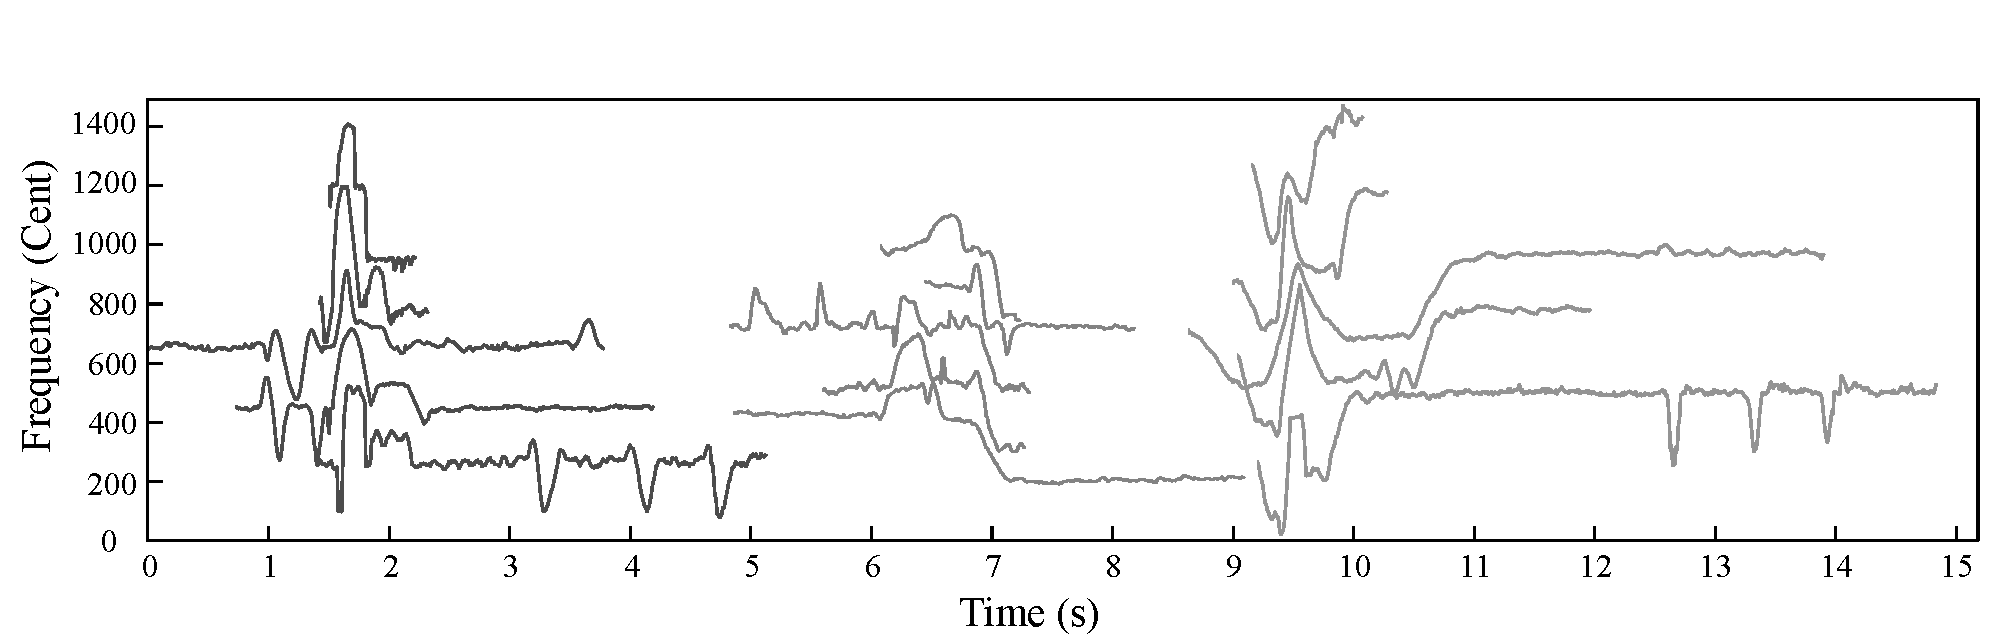
\includegraphics[width=\figSizeHundred]{ch06_patterns/figures/ImprovingSimilarity/phraseClassesExample_BW.pdf}
		\else
			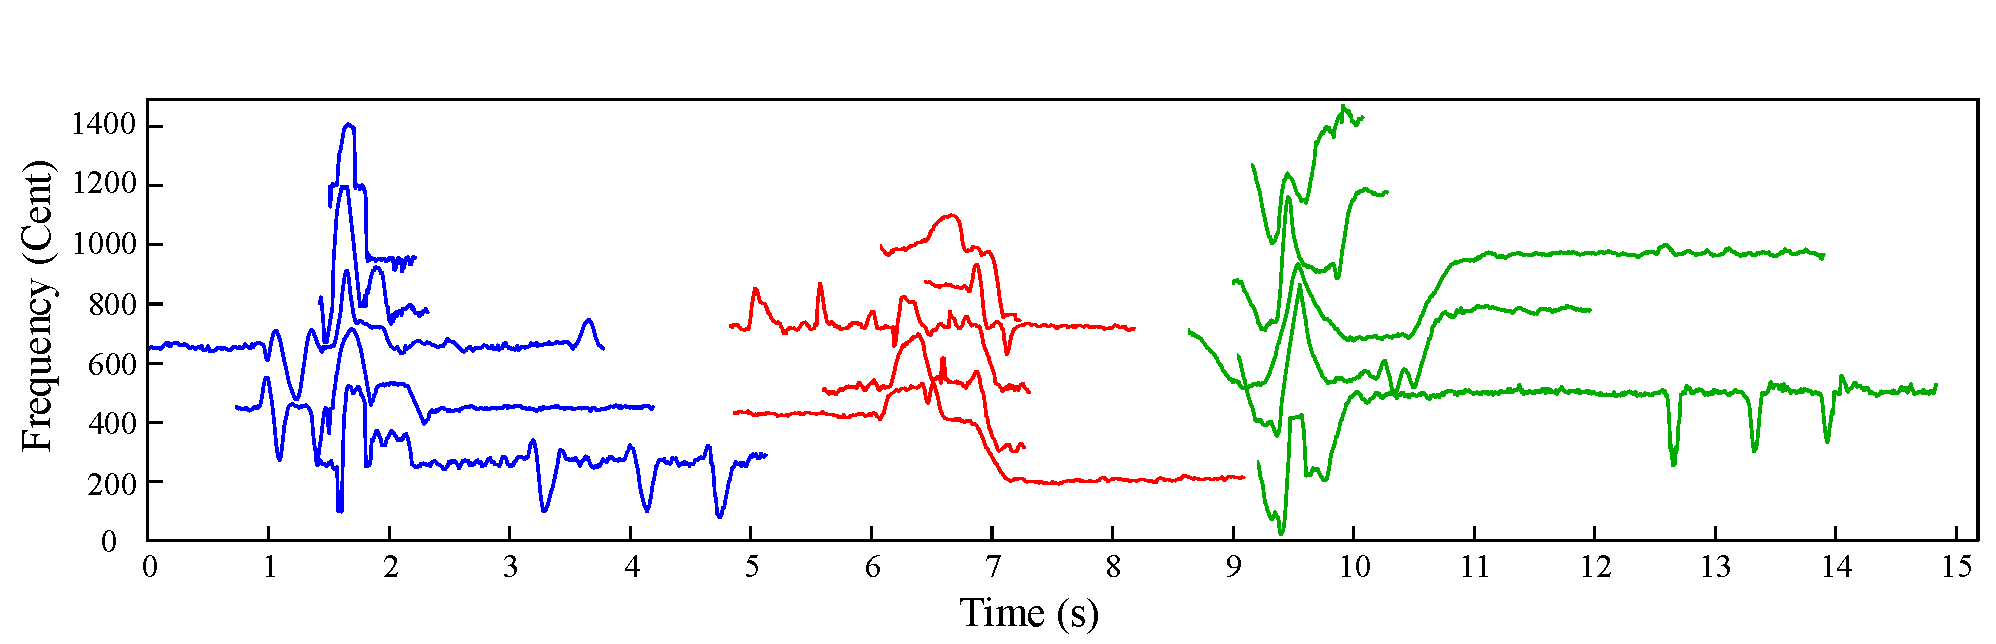
\includegraphics[width=\figSizeHundred]{ch06_patterns/figures/ImprovingSimilarity/phraseClassesExample.pdf}
		\fi
	\end{center}
	\caption[Examples of different occurrences of the \gls{raga} motifs]{Pitch contours of occurrences of three different characteristic melodic phrases in Hindustani music. Contours are frequency transposed and time shifted for a better visualization.}
	\label{fig:phraseComplexityExample}
\end{figure}

Before proceeding further it is worth revising the main challenges involved in the computation of melodic similarity for characteristic melodic phrases of \glspl{raga}. As already mentioned, the characteristic melodic phrases act as the basis for the artists to improvise, providing them with a medium to express creativity during a \gls{raga} rendition. Hence, the surface representation of these melodic phrases can vary a lot across their occurrences. This high degree of variability in terms of the duration of a phrase, non-linear time warping and the added melodic ornaments together pose a big challenge for melodic similarity computation. In Figure~\ref{fig:phraseComplexityExample} we illustrate this variability by showing the pitch contours of the different occurrences of three characteristic melodic phrases of the \gls{raga} \gls{alahaiya_bilaval}. We can clearly see that the duration of a phrase across its occurrences varies a lot and the steady melodic regions are highly varied in terms of the duration and the presence of melodic ornaments. Because of these factors detecting the occurrences of characteristic melodic phrases becomes a challenging task. Ideally, a melodic similarity measure should be robust to such high degree of melodic variations and, at the same time, it should be able to discriminate between different phrase categories and irrelevant melodic fragments (noise candidates).

In this section, we present two approaches that utilize specific melodic characteristics in \gls{iam} to improve melodic similarity. We describe a melodic abstraction process based on a partial transcription of melodies to handle large timing variations across occurrences of melodic phrases. Specifically for Carnatic music we also present a complexity weighting scheme that accounts for the differences in the melodic complexities of the phrases, a crucial aspect for melodic similarity in this music tradition. The following sections are based on our work presented in~\cite{gulati_ISMIR_2015}.

%\COMMENT{Highlight that we are incorporating and exploiting universal or transversal kind of characteristics. Specific nuances which are often raga specific and are very important for melodic similarity might be not possible since we do not have comprehensive annotated dataset.}


\subsection{Method}
\label{sec:patterns_improving_similarity_method}

\begin{figure}
	\begin{center}
		\ifdefined\PRINTVER
			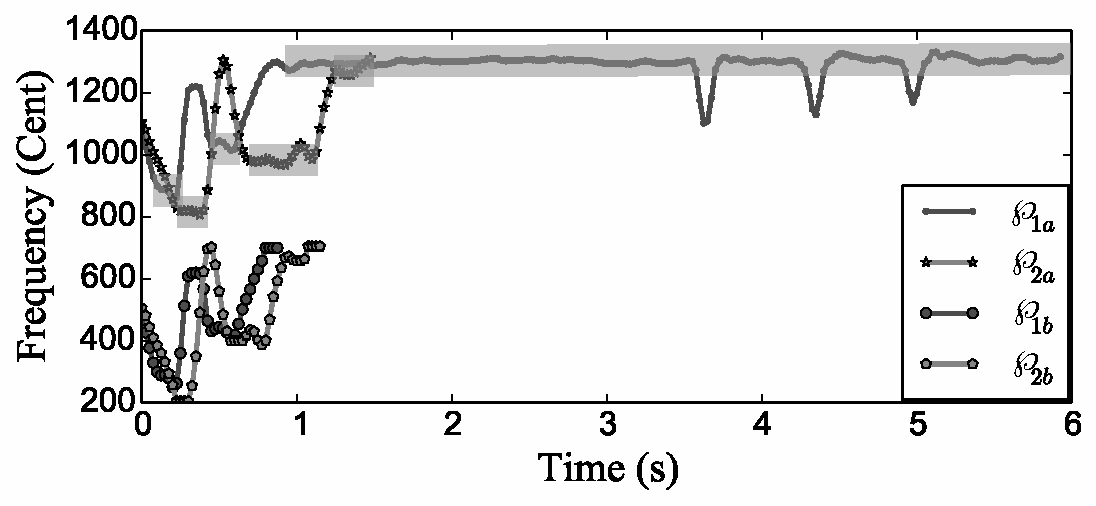
\includegraphics[width=\figSizeEightyFive]{ch06_patterns/figures/ImprovingSimilarity/Hindusani_flat_note_compression_example_reversed_BW.pdf}
		\else
			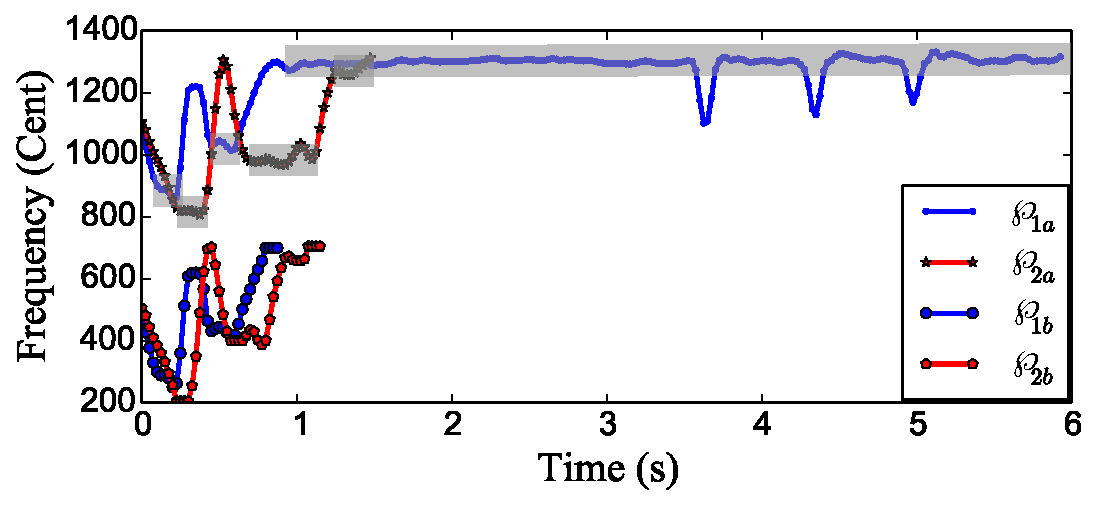
\includegraphics[width=\figSizeEightyFive]{ch06_patterns/figures/ImprovingSimilarity/Hindusani_flat_note_compression_example_reversed.pdf}
		\fi
	\end{center}
	\caption[Examples of melodic patterns after duration truncation]{Original pitch contours ($\pattern_{1a}$, $\pattern_{2a}$) and duration truncated pitch contours ($\pattern_{1b}$, $\pattern_{2b}$) of two occurrences of a characteristic phrase of \gls{raga} \gls{alahaiya_bilaval}. The contours are transposed for a good visualization.}
	\label{fig:flatCompressionExample}
\end{figure}



Before we present our approach in detail we first discuss the motivation and rationale behind it. A close examination of the occurrences of the characteristic melodic phrases in our dataset reveals that there is a pattern in the non-linear timing variations, which is also reported in~\cite{Rao2014}. In~\figref{fig:phraseComplexityExample} we show a few occurrences of three such melodic phrases. In particular, we see that the transient regions of a melodic phrase tend to span nearly the same time duration across different occurrences, whereas the stationary regions vary a lot in terms of the duration. In~\figref{fig:flatCompressionExample} we further illustrate this by showing two occurrences of a melodic phrase ($\pattern_{1a}$ and $\pattern_{2a}$). The stationary \gls{svara} regions are highlighted. We clearly see that the duration variation is prominent in the highlighted regions. To handle such large non-linear timing variations typically a non-constrained \gls{dtw} distance measure is employed~(\secref{sec:patterns_melodic_similarity_results_discussions}). However, such a \gls{dtw} variant is prone to noisy matches. Moreover, the absence of a band constraint renders it inefficient for computationally complex tasks such as pattern discovery~(\secref{sec:patterns_melodic_pattern_discovery}).



We put forward an approach that abstracts the melodic representation and reduces the extent of duration and pitch variations across the occurrences of a melodic phrase. Our approach is based on the partial transcription of the melodies. As mentioned earlier, melodic transcription in \gls{iam} is a challenging task. The main challenges arise due to the presence of non-discrete pitch movements such as smooth glides and \glspl{gamaka}. However, since the duration variation exists mainly during the steady \gls{svara} regions, transcribing only the stable melodic regions might be sufficient. Once transcribed, we can then truncate the duration of these steady melodic regions and hence effectively reduce the amount of timing variations across the occurrences of a melodic phrase. Additionally, since the duration truncation also reduces the overall length of a pattern, the computational time for melodic similarity computation is also reduced substantially. Furthermore, this solution is independent of the distance measure used in the melodic similarity computation. Hence, it can be used even in the computationally complex tasks such as large scale pattern discovery, where the usage of distance lower bounds is imperative~(\secref{sec:patterns_melodic_pattern_discovery}).

\begin{figure}
	\begin{center}
		\ifdefined\PRINTVER
			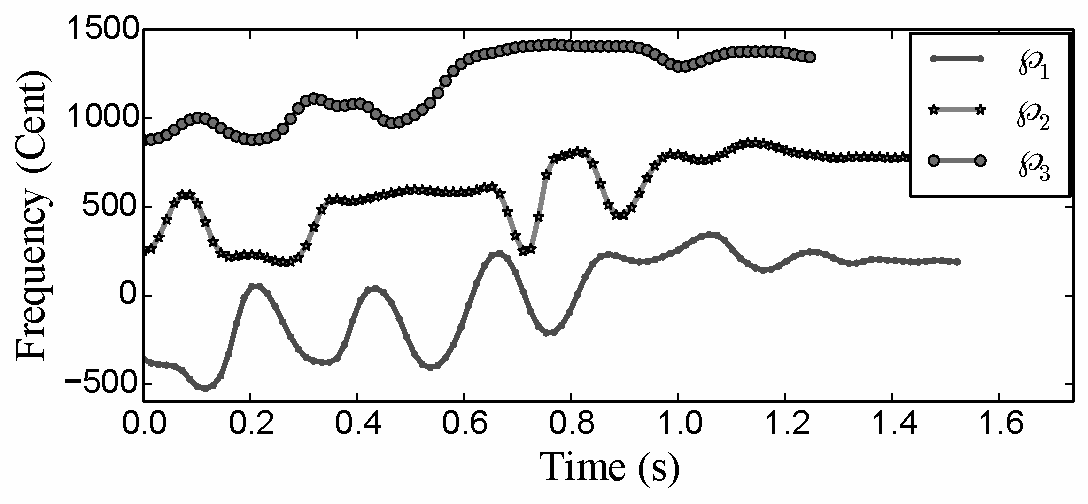
\includegraphics[width=\figSizeEighty]{ch06_patterns/figures/ImprovingSimilarity/CarnaticComplexityExample_BW.pdf}
		\else
			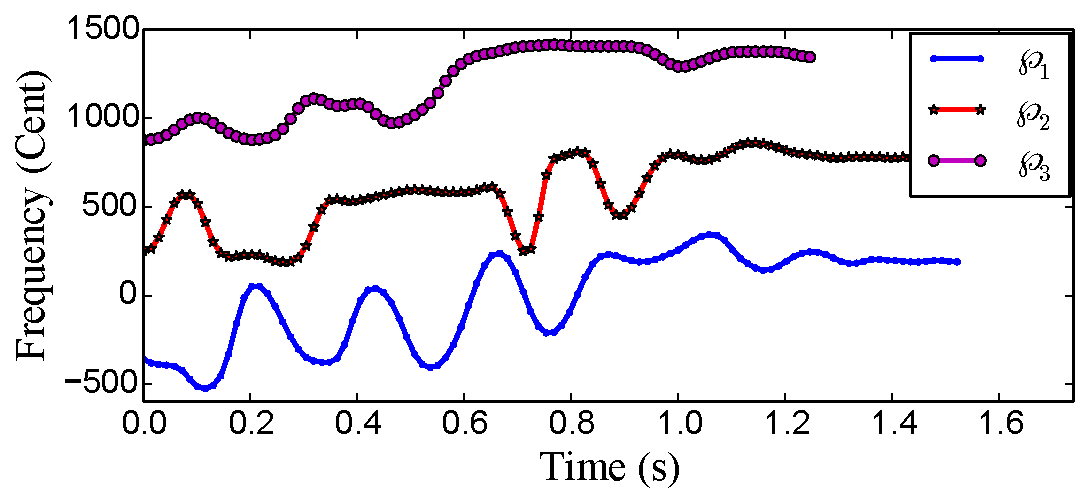
\includegraphics[width=\figSizeEightyFive]{ch06_patterns/figures/ImprovingSimilarity/CarnaticComplexityExample.pdf}
		\fi		
	\end{center}
	\caption[Illustration of an erroneous case of melodic similarity in Carnatic music]{Pitch contours of three melodic phrases ($\pattern_1$, $\pattern_2$, $\pattern_3$). $\pattern_1$ and $\pattern_2$ are the occurrences of the same characteristic phrase and both are musically dissimilar to $\pattern_3$.} 
	\label{fig:carnaticComplexityExample}
\end{figure}

The rapid oscillatory pitch movements (\glspl{gamaka}) in Carnatic music bring up another set of challenges for the melodic similarity computation. Very often, two musically dissimilar melodic phrases obtain a high similarity score owing to a similar pitch contour at a macro level. However, they differ significantly at a micro level. In~\figref{fig:carnaticComplexityExample} we illustrate such a case where we show the pitch contours of three melodic phrases $\pattern_1$, $\pattern_2$ and $\pattern_3$, where $\pattern_1$ and $\pattern_2$ are the occurrences of the same melodic phrase and both are musically dissimilar to $\pattern_3$. Using the best performing variant of the similarity measure obtained in~\secref{sec:patterns_melodic_similarity_results_discussions} (\tabref{tab:melodic_similarity_results}) we obtain a higher similarity score between the pairs ($\pattern_1$, $\pattern_3$) and ($\pattern_2$, $\pattern_3$) compared to the score between the pair ($\pattern_1$, $\pattern_2$). This tendency of a high complexity time-series (higher degree of micro level variations) obtaining a high similarity score with another low complexity time-series is discussed in~\cite{batista2011complexity}. We follow their approach and apply a complexity weighting to account for the differences in the melodic complexities between phrases in the computation of melodic similarity. 


We now proceed to describe our method in detail. The block diagram for computing melodic similarity is very similar to the one described in~\secref{sec:method_similarity_evaluation}. The main differences are the added processing blocks for performing partial transcription, \gls{svara} duration truncation and complexity weighting as shown in~\figref{fig:block_diagram_melodic_similarity_improved}. In the subsequent sections we describe every processing block in detail. 

\begin{figure}
	\begin{center}
		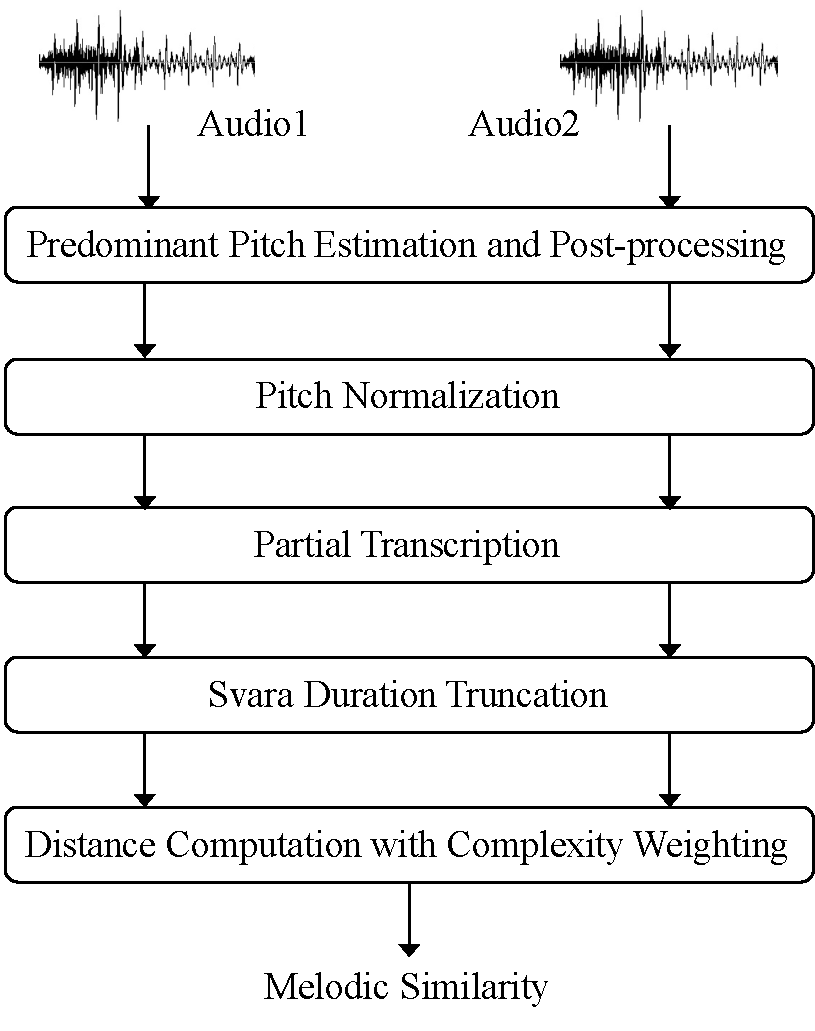
\includegraphics[width=\figSizeSixty]{ch06_patterns/figures/ImprovingSimilarity/melodic_similarity_improve_blockd.pdf}
	\end{center}
	\caption[Block diagram for an improved melodic similarity computation]{Block diagram of the improved methodology for computing melodic similarity.} 
	\label{fig:block_diagram_melodic_similarity_improved}
\end{figure}

\subsubsection{Predominant Pitch Estimation and post-processing}
\label{sec:patterns_improving_similarity_melody_estimation}

As done before, we represent melody of an audio signal by the pitch of the predominant melodic source. For predominant pitch estimation we follow exactly the same procedure and use the same parameter values as done in~\secref{sec:patterns_melodic_similarity_representation}, which is explained in detail in~\secref{sec:data_preprocessing_predominant_melody_estimation}. After estimating the predominant pitch we convert it from Hertz to Cent scale for the melody representation to be musically relevant~(\secref{sec:data_processing_cent_conversion}).

We proceed to post-process the pitch contours to remove the spurious pitch jumps lasting over a few frames as well as to smooth the pitch contours. We follow the procedure described in~\secref{sec:data_processing_pitch_smoothening} and use exactly the same set of parameter values. The pitch contours are finally down-sampled to 67\,Hz (\secref{sec:data_processing_pitch_resampling}). This sampling rate was found to be working well for both Carnatic and Hindustani music in our earlier study that evaluated five different sampling rates~\secref{sec:patterns_melodic_similarity_results_discussions}.


\subsubsection{Pitch Normalization}
\label{sec:patterns_improving_similarity_transposition_invariance}

The base frequency chosen for a melody in \gls{iam} is the tonic pitch of the lead artist~(\secref{sec:data_preprocessing_tonic_identification}). Therefore, for a meaningful comparison of the melodic phrases across the recordings of different artists, a melody representation should be normalized by the tonic pitch of the lead artist. We perform this tonic normalization ($\mNorm_\mathrm{tonic}$) by considering the tonic of the lead artist as the reference frequency during the Hertz to Cent conversion as shown in~\secref{sec:data_processing_cent_conversion}. The tonic pitch is automatically identified using \acrshort{tonicid_justin} method, which performed the best in our comparative evaluation of seven different approaches~(\secref{sec:pre_processing_tonic_identification_results}).

Tonic normalization does not account for the pitch of the octave transposed occurrences of a melodic phrase within a recording. In addition, estimated tonic pitch sometimes might be incorrect and a typical error is an offset of an octave or a fifth scale degree in some cases. To handle such cases, we propose a tetrachord normalization ($\mNorm_\mathrm{tetra}$). For this we analyse the difference ($\pitchDiff_m$) in the mean frequency values of the two tonic normalized melodic phrases ($\pattern_1$, $\pattern_2$). We offset the pitch values of the phrase $\pattern_1$ by the frequency (Cents) in the set $\lbrace$-\,1200, -\,700, -\,500, 0, 500, 700, 1200, 1700, 1900$\rbrace$ that is closest to $\pitchDiff_m$ within a vicinity of 100\,Cents. In addition to tetrachord normalization, we also experiment with mean normalization ($\mNorm_\mathrm{mean}$), which was reported to improve the performance in the case of Carnatic music~(\secref{sec:patterns_melodic_similarity_results_discussions}). 


\subsubsection{Partial Transcription}
\label{sec:patterns_improving_similarity_partial_transcription}

We perform a partial melody transcription to automatically segment and identify the steady \gls{svara} regions in a melody. Note that even a partial transcription of the melodies is a non-trivial task, since we desire a segmentation that is robust to different melodic ornaments added to a \gls{svara} where the pitch deviation from the mean \gls{svara} frequency can be up to 200\,Cents. In~\figref{fig:flatCompressionExample} we show such an example of a steady \gls{svara} region ($\pattern_{1a}$ from 3-6\,s) where the pitch deviation from the mean \gls{svara} frequency is high due to added melodic ornaments. Ideally, the melodic region between 1 and 6\,s should be detected as a single \gls{svara} segment.

We segment the steady \gls{svara} regions using a method described in~\cite{gulati2014Landmark} (\secref{sec:pre_processing_nyas_segmentation}), which addresses the aforementioned challenges. A segmented \gls{svara} region is then assigned a frequency value corresponding to the peak in an aggregated pitch histogram closest to the mean \gls{svara} frequency. The pitch histogram is constructed for the entire recording and smoothened using a Gaussian window with a variance of 15\,Cents. As peaks of the normalized pitch histogram, we select all the local maximas where at least one peak-to-valley ratio is greater than 0.01. A detailed description of this method is provided in~\secref{sec:pre_processing_nyas_segmentation}.
 
\subsubsection{Svara Duration Truncation}
\label{sec:patterns_improving_similarity_svara_duration_trucation}

After segmenting the steady \gls{svara} regions in the melodies we proceed to truncate the duration of these regions. We hypothesize that, beyond a certain value $\svarTruncThsld$, the duration of these steady \gls{svara} regions do not change the identity of a melodic phrase (i.e.~the phrase category). We experiment with 7 different truncation durations $\svarTruncThsld = \lbrace$ 0.1\,s, 0.3\,s, 0.5\,s, 0.75\,s, 1\,s, 1.5\,s, 2\,s$\rbrace$ and select the one that results in the best performance. In~\figref{fig:flatCompressionExample}
we show an example of the occurrences of a melodic phrase both before ($\pattern_{1a}$, $\pattern_{2a}$) and after ($\pattern_{1b}$, $\pattern_{2b}$) the \gls{svara} duration truncation using $\svarTruncThsld = 0.1$\,s. This example clearly illustrates that the occurrences of a melodic phrase after duration truncation exhibit lower degree of non-linear timing variations. We denote this method by \acrshort{similarity_dt}.

\subsubsection{Distance Computation}
\label{sec:patterns_improving_similarity_similarity_computation}

To measure the similarity between two melodic fragments we consider a \gls{dtw}-based distance measure. Since the phrase segmentation is known beforehand, we use a whole sequence matching \gls{dtw} variant. We consider the best performing \gls{dtw} variant and the related parameter values for each music tradition as reported in~\secref{sec:patterns_melodic_similarity_results_discussions}. These variants were chosen based on an exhaustive grid search across all possible combinations and hence can be considered as optimal for this dataset. We use Sakoe-Chiba global band constraint~\cite{Sakoe78TASLP} with the width of the band as $\pm10$\% of the phrase length. Before computing the \gls{dtw} distance we uniformly time-scale the two melodic fragments to the same length, which is the maximum of the lengths of the phrases. Notice that even though in~\secref{sec:patterns_melodic_similarity_results_discussions} we found that a globally unconstrained \gls{dtw} variant ($\distPattMeasure_{\mathrm{DTW\_L0\_G90}}$) is an optimal choice for computing melodic similarity in Hindustani music, we restrict ourselves to a band-width of 10\% in this study. The main reason is because an unconstrained \gls{dtw} variant due to its computational complexity is not suitable for a large scale pattern discovery task~(\secref{sec:patterns_melodic_pattern_discovery}). Since one the main objectives of studying melodic similarity within a supervised setup in this work is to be finally able to apply the findings in an unsupervised analysis, we now restrict to choices that are also available and feasible in an unsupervised analysis.


\subsubsection{Complexity Weighting}
\label{sec:patterns_improving_similarity_complexity_invariance_weighting}

The complexity weighting that we apply here to overcome the shortcoming of the distance measure in distinguishing two time series with different complexities is discussed in~\cite{batista2011complexity}. We apply a complexity weighting ($\compWght$) to the \gls{dtw}-based distance ($\distPattMeasure_\mathrm{DTW}$) in order to compute the final similarity score $\distPattMeasure_{f}=\compWght \distPattMeasure_\mathrm{DTW}$. We compute $\compWght$ as:


\begin{equation}
\begin{gathered}
\compWght = \frac{\max(\compEst_i,\compEst_j)}{\min(\compEst_i, \compEst_j)} \\
%\compEst_i = \sqrt[2]{\sum_{i=1}^{N-1} (\pitchCents_{i}-\pitchCents_{i+1})^2}\\
\end{gathered}
\label{eq:complexity_weighing}
\end{equation}

\begin{equation}
\begin{gathered}
%\compWght = \frac{\max(\compEst_i,\compEst_j)}{\min(\compEst_i, \compEst_j)} \\
\compEst_i = \sqrt[2]{\sum_{i=1}^{N-1} (\pitchCents_{i}-\pitchCents_{i+1})^2}\\
\end{gathered}
\label{eq:complexity_estimate_batista}
\end{equation}

\noindent where, $\compEst_i$ is the complexity estimate of a melodic pattern of length $N$ samples and $\pitchCents_i$ is the pitch value of the $i^{\mathrm{th}}$ sample. We explore two variants of this complexity estimate. One of these variants is already proposed in~\cite{batista2011complexity} and is described in~\eqnref{eq:complexity_estimate_batista}. We denote this method variant by \acrshort{similarity_cw1}. We propose another variant that utilizes melodic characteristics of Carnatic music. This variant takes the number of saddle points in the melodic phrase as the complexity estimate~\citep{Ishwar2013}. This method variant is denoted by \acrshort{similarity_cw2}. As saddle points we consider all the local minimas and the local maximas in the pitch contour which have at least one minima to maxima distance of half a semitone. Since such melodic characteristics are predominantly present in Carnatic music, the complexity weighting is not applicable for computing melodic similarity in Hindustani music.


\subsection{Evaluation}
\label{sec:patterns_improving_similarity_evaluation}

\subsubsection{Dataset and Annotations}
\label{sec:patterns_improving_similarity_dataset_and_annotations}

For evaluation we use the same music collection as used in~\secref{sec:patterns_evaluation_of_similarity_measures}, which is described in~\secref{sec:corpus_melodic_similarity_dataset}. This collection enables a better comparison of the results with other studies since it has been used in several other studies for a similar task~\citep{Rao2014,Ross2012b}. However, we found a number of issues in the annotations of the melodic phrases, which we corrected and also extended the dataset by adding 25\% more number of melodic phrase annotations as explained in~\secref{sec:corpus_melodic_similarity_dataset}. We denote this new dataset by \acrshort{msds_cm} and the comprising Carnatic and Hindustani sub-datasets by \acrshort{msds_cm_cmd} and \acrshort{msds_cm_hmd}, respectively. Similar to the way we perform evaluations in~\secref{sec:patterns_evaluation_of_similarity_measures}, we evaluate our approach separately on both Carnatic and Hindustani datasets. In~\tabref{tab:melodic_similarity_dataset_details} we summarize the relevant details of the dataset in terms of the number of artists, \glspl{raga}, audio recordings and total duration. In~\tabref{tab:categorywise_details_revised_melodic_similarity_dataset} we summarize the details of the annotated phrases in terms of their number of instances and basic statistics of the length of the phrases.


\subsubsection{Setup, Measures and Statistical Significance}
\label{sec:patterns_improving_similarity_experimental_setup}

The experimental setup and evaluation measures used in this study are exactly the same as used for the comparative evaluation described in~\secref{sec:patterns_evaluation_of_similarity_measures}. We consider each annotated melodic phrase as a query and perform a search across all the annotated phrases in the dataset (referred to as target search space). In addition to the annotated phrases, we add randomly sampled melodic segments (referred to as noise candidates) in the target space to simulate a real world scenario. We generate the starting time stamps of the noise candidates by randomly sampling a uniform distribution. The length of the noise candidates are generated by sampling the distribution of the duration values of the annotated phrases. The number of noise candidates added are 100 times the number of total annotations in the entire music collection. For every query we consider the top 1000 nearest neighbors in the search results ordered by the similarity value. A retrieved melodic phrase is considered as a true hit only if it belongs to the same phrase category as the query. As a baseline in this study we consider the same method as described in this section but without applying the \gls{svara} duration truncation and complexity weighting procedure. We denote this baseline method by \acrshort{similarity_b}.

To assess the performance of our approach and the baseline method we use \acrfull{map}, a common measure in information retrieval~\citep{manning2008introduction}. To assess if the difference in the performance of any two methods is statistically significant we use the Wilcoxon signed rank-test~\citep{wilcoxon1945individual} with $\pVal < 0.01$. To compensate for multiple comparisons, we apply the Holm-Bonferroni met-hod~\citep{holm1979simple}.


\subsection{Results and Discussion}
\label{sec:patterns_improving_similarity_results_and_discussion}

%\COMMENT{if time permits, first report the accuracy of best variants of prev study on new dataset an then with post processing, and then with new method?, also the chosen config in the current study, it should be shown how that is behaving in previous study. Also should we also present var2 of our approach, i.e. with unknown segment lengths?}
%\COMMENT{If time permits also experiment with NCR1, 10, 100, 1000 for the best config. That way we can know what is the affect of NCR!!}

In~\tabref{tab:patterns_improving_similarity_map_scores} we summarize the \gls{map} scores and the standard deviation of the average precision values obtained using the baseline method (\acrshort{similarity_b}), the method that uses duration truncation (\acrshort{similarity_dt}) and the ones using the complexity weighting (\acrshort{similarity_cw1}, \acrshort{similarity_cw2}), for both the \acrshort{msds_cm_cmd} and the \acrshort{msds_cm_hmd}. Note that \acrshort{similarity_cw1} and \acrshort{similarity_cw2} are only applicable to the \acrshort{msds_cm_cmd} (\secref{sec:patterns_improving_similarity_complexity_invariance_weighting}).


\begin{table} 
	\begin{centering}
	\tabcolsep = 0.15cm
	\renewcommand{\arraystretch}{1.5}
	\begin{tabular}{ c | c  c  c  c }
\tabletop
		\multicolumn{5}{c }{\acrshort{msds_cm_hmd}}\\
\tablemid
		Norm &	\acrshort{similarity_b} & \acrshort{similarity_dt} &  \acrshort{similarity_cw1} & \acrshort{similarity_cw2}\\
\tablemid		
		$\mNorm_\mathrm{tonic}$	& {\bf 0.45 (0.25)}	&	{\bf 0.52 (0.24)} 	& - &-\\ 
		$\mNorm_\mathrm{mean}$	& 0.25 (0.20)		&	0.31 (0.23) 		& - &-\\  	
		$\mNorm_\mathrm{tetra}$	& 0.40 (0.23)		&	0.47 (0.23) 		& - &-\\  	
		
		%& $E_2$ & xxx	& 0.25	&	0.27 & - \\   
\tablebot
		\multicolumn{5}{c }{\acrshort{msds_cm_cmd}}\\
\tablemid
		Norm &	\acrshort{similarity_b} & \acrshort{similarity_dt} &  \acrshort{similarity_cw1} & \acrshort{similarity_cw2}\\
		\hline
		$\mNorm_\mathrm{tonic}$	&  0.39 (0.29)	&	0.42 (0.29) & 0.41 (0.28)&0.41 (0.29) \\ 
		$\mNorm_\mathrm{mean}$	&  0.39 (0.26)	&	0.45 (0.28) & 0.43 (0.27)&0.45 (0.27) \\  	
		$\mNorm_\mathrm{tetra}$	&  {\bf 0.45 (0.26)}	&	{\bf 0.50 (0.27)} & {\bf 0.49 (0.28)} &{\bf 0.51 (0.27)} \\  	
\tablebot	
		
	\end{tabular}
	\caption[\acrshort{map} scores for \acrshort{msds_cm_hmd} and \acrshort{msds_cm_cmd} datasets obtained by \acrshort{similarity_b}, \acrshort{similarity_dt}, \acrshort{similarity_cw1} and \acrshort{similarity_cw2}]{\acrshort{map} scores for the two datasets \acrshort{msds_cm_hmd} and \acrshort{msds_cm_cmd} for the four method variants \acrshort{similarity_b}, \acrshort{similarity_dt}, \acrshort{similarity_cw1} and \acrshort{similarity_cw2} and for different normalization techniques. Standard deviation of average precision is reported within round brackets.}
	\label{tab:patterns_improving_similarity_map_scores}
\par \end{centering}	
\end{table}

\begin{figure}[h]
	\begin{center}
		\ifdefined\PRINTVER
			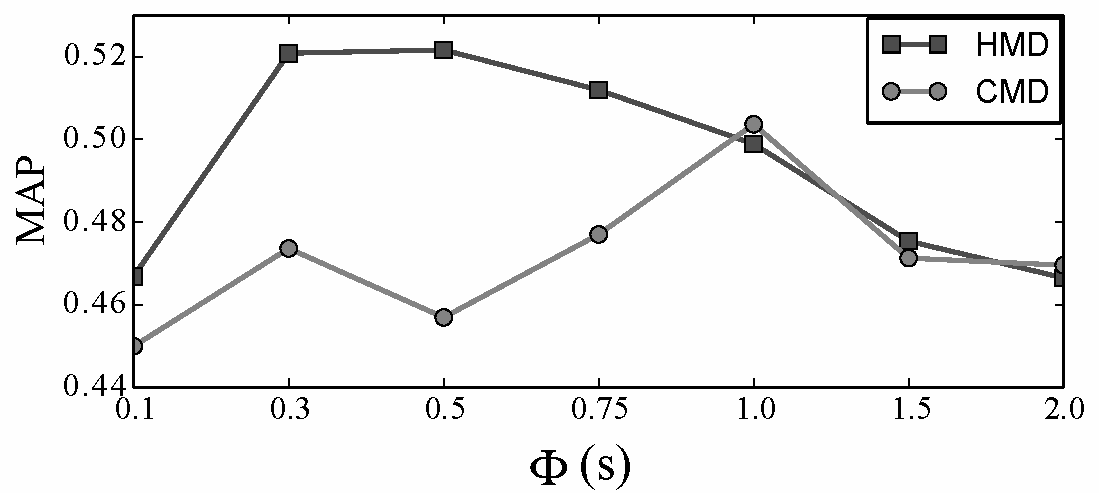
\includegraphics[width=\figSizeEightyFive]{ch06_patterns/figures/ImprovingSimilarity/MAP_per_Duration_Truncation_BW.pdf}
		\else
			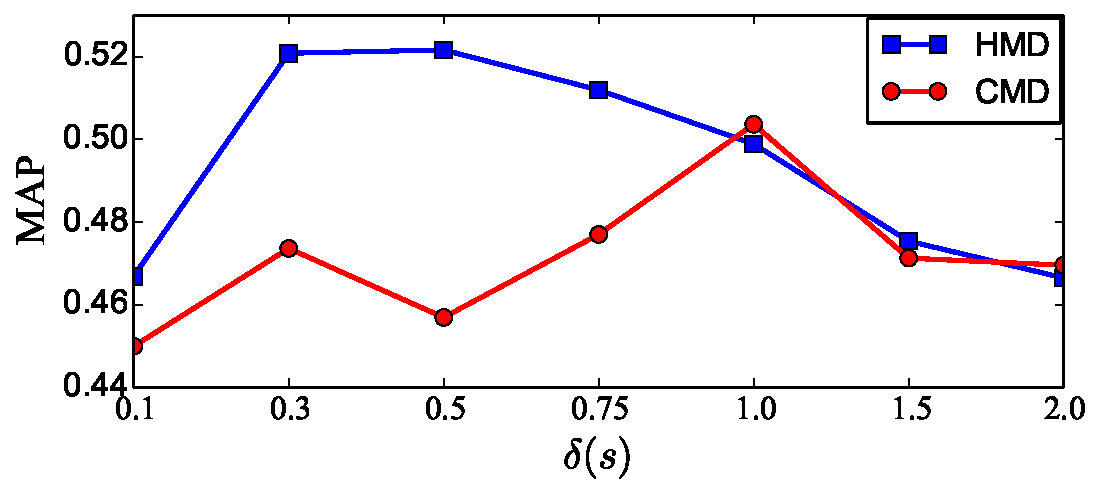
\includegraphics[width=\figSizeEightyFive]{ch06_patterns/figures/ImprovingSimilarity/MAP_per_Duration_Truncation.pdf}
		\fi
	\end{center}
	\caption[\acrshort{map} scores for different duration truncation values]{\gls{map} scores for different duration truncation values ($\svarTruncThsld$) for the \acrshort{msds_cm_hmd} and the \acrshort{msds_cm_cmd}. Only the superscript in the name of the dataset is used in the figure legend.} 
	\label{fig:map_per_duration_truncation}
\end{figure}

We first analyse the results for the \acrshort{msds_cm_hmd} dataset. From~\tabref{tab:patterns_improving_similarity_map_scores} (upper half), we see that the proposed method variant that applies a duration truncation performs better than the baseline method for all the normalization techniques. Moreover, this difference is found to be statistically significant in each case. The results for the \acrshort{msds_cm_hmd} in this table correspond to $\svarTruncThsld=$500\,ms, for which we obtain the highest accuracy compared to the other $\svarTruncThsld$ values as shown in~\figref{fig:map_per_duration_truncation}. Furthermore, we see that $\mNorm_\mathrm{tonic}$ results in the best accuracy for the \acrshort{msds_cm_hmd} for all the method variants and the difference is found to be statistically significant in each case. From~\tabref{tab:patterns_improving_similarity_map_scores} we notice a high standard deviation of the average precision values. This is because some occurrences of melodic phrases possess a large amount of melodic variation (acting as outliers), and therefore, the average precision value of the retrieved results using them as a query is much smaller compared to the other occurrences. In~\figref{fig:hinudstaniPerCategoryPerformance} we show a boxplot of average precision values for each phrase category and for both \acrshort{similarity_b} and \acrshort{similarity_dt} to get a better understanding of the results. We observe that with an exception of the phrase category $H_2$, \acrshort{similarity_dt} consistently performs better than \acrshort{similarity_b} for all the other phrase categories. A close examination of this exception reveals that the error often is in the segmentation of the steady \gls{svara} regions of the melodic phrases corresponding to $H_2$. This can be attributed to a specific subtle melodic movement in $H_2$ that is confused by the segmentation method as a melodic ornament instead of a \gls{svara} transition, leading to a segmentation error.%\COMMENT{If time permits show an image of this pattern and the subtle movement!! if you plot images for all the patterns in the dataset refer to that}


\begin{figure}
	\begin{center}
		\ifdefined\PRINTVER
			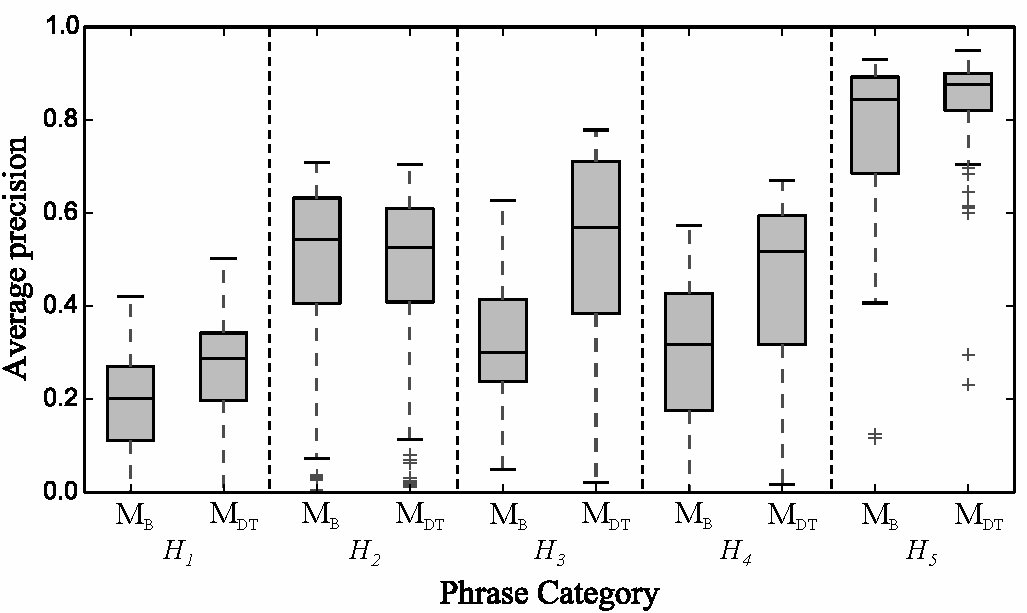
\includegraphics[width=\figSizeNinety]{ch06_patterns/figures/ImprovingSimilarity/HindustaniPerCategoryPerformance_BOXPLOT_BW.pdf}
		\else
			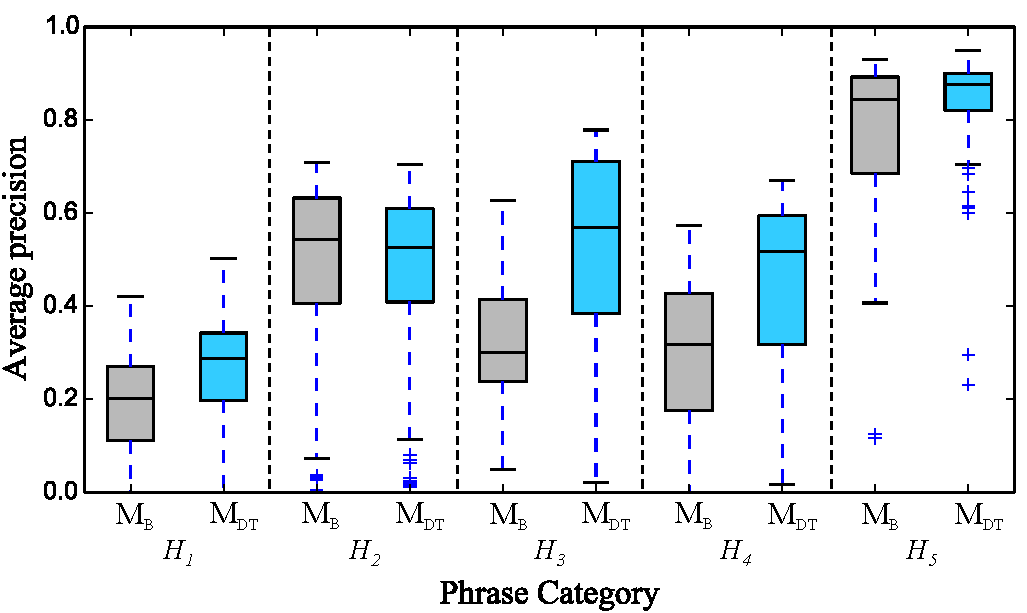
\includegraphics[width=\figSizeNinety]{ch06_patterns/figures/ImprovingSimilarity/HindustaniPerCategoryPerformance_BOXPLOT.pdf}
		\fi
	\end{center}
	\caption[Boxplot of average precision for different types of melodic patterns in the Hindustani music dataset]{Boxplot of average precision values obtained using \acrshort{similarity_b} and \acrshort{similarity_dt} for each melodic phrase category for the \acrshort{msds_cm_hmd}. These values correspond to $\mNorm_\mathrm{tonic}$.} 
	\label{fig:hinudstaniPerCategoryPerformance}
\end{figure}


We now analyse the results for the \acrshort{msds_cm_cmd} dataset. From~\tabref{tab:patterns_improving_similarity_map_scores} (lower half), we see that using the method variants \acrshort{similarity_dt}, \acrshort{similarity_cw1} and \acrshort{similarity_cw2} we obtain reasonably higher \gls{map} scores compared to the baseline method \acrshort{similarity_b} and the difference is found to be statistically significant for each method variant across all normalization techniques. This \gls{map} score for \acrshort{similarity_dt} corresponds to $\svarTruncThsld=$1\,s, which is considerably higher than the \gls{map} scores for other $\svarTruncThsld$ values as shown in~\figref{fig:map_per_duration_truncation}. We also see that \acrshort{similarity_cw2} performs slightly better than \acrshort{similarity_cw1} and the difference is found to be statistically significant only in the case of $\mNorm_\mathrm{tetra}$. We do not find any statistically significant difference in the performance of methods \acrshort{similarity_dt} and \acrshort{similarity_cw2}. Unlike in the case of the \acrshort{msds_cm_hmd} dataset, for the \acrshort{msds_cm_cmd} dataset $\mNorm_\mathrm{tetra}$ results in the best performance with a statistically significant difference compared to the other normalization techniques across all method variants. We now analyse the average precision values for every phrase category for \acrshort{similarity_b}, \acrshort{similarity_dt} and \acrshort{similarity_cw2}. Since \acrshort{similarity_cw2} performs slightly better than \acrshort{similarity_cw1} we only consider \acrshort{similarity_cw2} for this analysis. In~\figref{fig:carnaticPerCategoryPerformance} we see that \acrshort{similarity_dt} performs better than \acrshort{similarity_b} for all phrase categories. We also observe that \acrshort{similarity_cw2} consistently performs better than \acrshort{similarity_b} with the sole exception of $C_2$. This exception occurs because \acrshort{similarity_cw2} presumes a consistency in terms of the number of saddle points across the occurrences of a melodic phrase, which does not hold true for $C_2$. This is because phrases corresponding to $C_2$ are rendered very fast and the subtle pitch movements are not the characteristic aspect of such melodic phrases. Hence, the artists often take the liberty of changing the number of saddle points. 

\begin{figure}
	\begin{center}
		\ifdefined\PRINTVER
			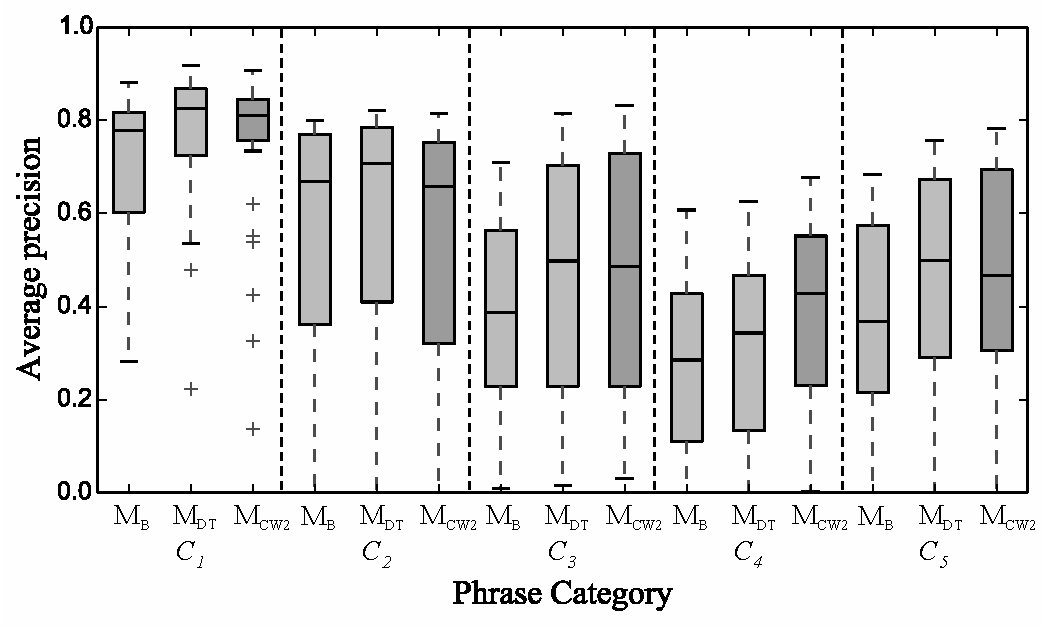
\includegraphics[width=\figSizeHundred]{ch06_patterns/figures/ImprovingSimilarity/CarnaticPerCategoryPerformance_BOXPLOT_BW.pdf}
		\else
			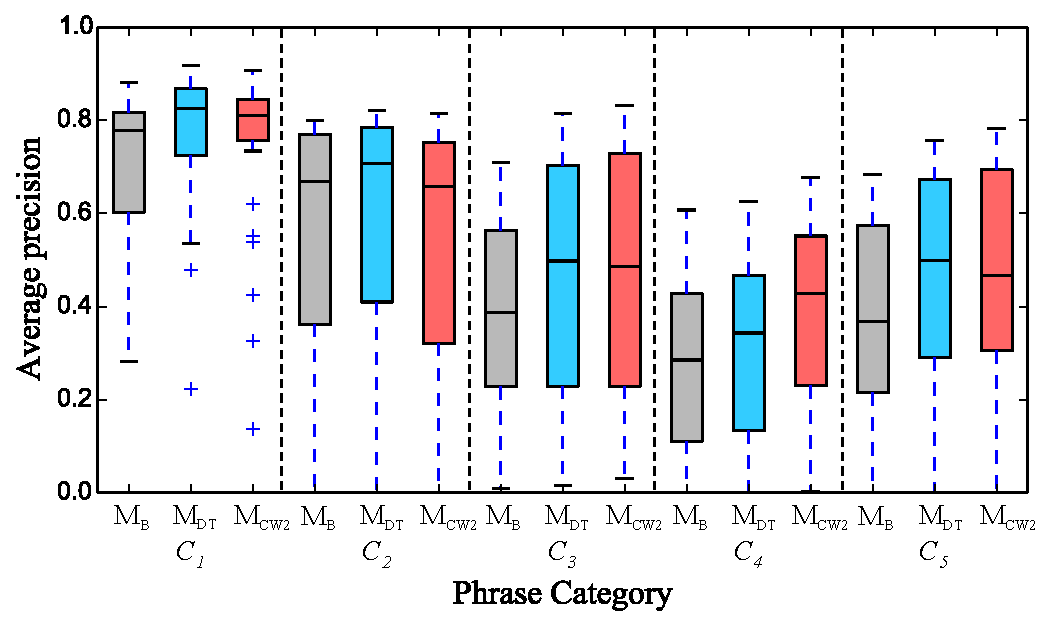
\includegraphics[width=\figSizeHundred]{ch06_patterns/figures/ImprovingSimilarity/CarnaticPerCategoryPerformance_BOXPLOT.pdf}
		\fi
	\end{center}
	\caption[Boxplot of average precision for different types of melodic patterns in the Carnatic music dataset]{Boxplot of average precision values obtained using methods \acrshort{similarity_b}, \acrshort{similarity_dt} and \acrshort{similarity_cw2} for each melodic phrase category for the \acrshort{msds_cm_cmd}. These values correspond to $\mNorm_\mathrm{tetra}$.}
	\label{fig:carnaticPerCategoryPerformance}
\end{figure}


Overall, we see that duration truncation of steady melodic regions improves the performance in both \acrshort{msds_cm_hmd} and \acrshort{msds_cm_cmd} datasets. This reinforces our hypothesis that elongation of steady \gls{svara} regions (up to a permissible limit) in the melodies of \gls{iam} in the context of the characteristic melodic phrase does not change the musical identity of the phrase. This correlates with the concept of \gls{nyas} \gls{svara} (\secref{sec:melody_in_iam}), where the artist has the flexibility to stay and elongate a single \gls{svara}. A similar observation was reported in~\cite{Rao2014}, where the authors proposed to learn the optimal global \gls{dtw} constraints a priori for each pattern category. However, as they report, their proposed solution could not improve the performance. Further comparing the results for the \acrshort{msds_cm_hmd} and \acrshort{msds_cm_cmd} datasets we notice that $\mNorm_\mathrm{tonic}$ results in the best performance for the \acrshort{msds_cm_hmd} and $\mNorm_\mathrm{tetra}$ for the \acrshort{msds_cm_cmd}. This can be attributed to the fact that the number of the pitch-transposed occurrences of a melodic phrase is significantly higher in the \acrshort{msds_cm_cmd} compared to the \acrshort{msds_cm_hmd} (\secref{sec:patterns_melodic_similarity_results_discussions}). Also, since the non-linear timing variability in the \acrshort{msds_cm_hmd} is very high, any normalization ($\mNorm_\mathrm{mean}$ or $\mNorm_\mathrm{tetra}$) that involves a decision based on the mean frequency of the phrase is likely to fail.


%################################################################################################################
%########################################### Melodic Pattern Discovery ##########################################
%################################################################################################################


\section{Melodic Pattern Discovery}
\label{sec:patterns_melodic_pattern_discovery}

As argued in \secref{sec:patterns_introduction} the potential of a pattern-based melodic analysis in characterization of \glspl{raga}, compositions and artists in \gls{iam} gets severely restricted in a supervised experimental setup. As described before, this is mainly due to the factors such as limited dataset size, knowledge bias and human errors in the melodic pattern corpus provided by domain experts. Therefore, to overcome these issues we follow an unsupervised methodology to discover melodic patterns in sizable audio music collections of \gls{iam}. Since a quantitative evaluation of an unsupervised method for sizable datasets is difficult and rather ill-defined, improving such methods and learning optimal values of the system parameters becomes a challenging task. We therefore studied the computation of melodic similarity, a crucial component in a melodic pattern discovery method in a supervised manner in \secref{sec:patterns_evaluation_of_similarity_measures} and \secref{sec:patterns_improving_melodic_similarity}. The learnings from these supervised studies loop back into our unsupervised melodic pattern discovery method presented in this chapter. 

From our literature review presented in \secref{sec:background_relevant_work_other_music} and \secref{sec:background_relevant_work_iam} we see that several approaches have been proposed for extracting different kinds of repeating structures in music, including long-duration repetitions such as different sections of a music piece~\citep{serra2012unsupervised,Goto06TASLP, paulus2010state}, relatively small-duration repetitions being themes, riffs~\citep{Hsu2001a}, and melodic motifs~\citep{meredith2002algorithms,collins2011improved,Janssen2013}. While there exists a number of approaches for motivic discovery in sheet music~\citep{meredith2002algorithms,Cambouropoulos2006,conklin2001representation,Lartillot2005}, there are fewer approaches that work on audio music recordings~\citep{dannenberg2003pattern}. This can be attributed to the audio-symbolic gap \citep{collins2014bridging}, which is argued to be bridged by a reliable automatic transcription system to abstract the audio music content into musically meaningful discrete symbols. Although, for several music traditions such as \gls{iam} melodic transcription still remains a challenging and a rather ill-defined task. A detailed account of the shortcomings in the existing pattern discovery methods in the context of their applicability to melodies in \gls{iam} is presented in our literature review in \secref{sec:sota_pattern_processing_iam} and \secref{sec:query_by_humming}. We see that there exists a wide scope for developing methodologies for the discovery and analysis of short duration melodic patterns (or motifs) in large audio music collections. Approaches for motif discovery can benefit from the literature in the domain of time series analysis such as time series representation~\citep{Lin2003}, core pattern discovery methods~\citep{Mueen2009}, and search and indexing techniques~\citep{Rakthanmanon2013}. We now proceed to describe our methodology for melodic pattern discovery in sizable audio music collections of \gls{iam}.


\subsection{Method}
\label{sec:patterns_discovery_method}

\begin{figure}
	\begin{center}
		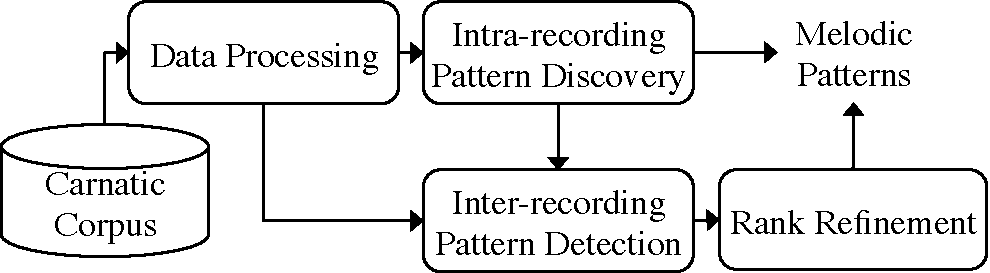
\includegraphics[width=\figSizeEightyFive]{ch06_patterns/figures/discovery/blockDiagram_Overall.pdf}
	\end{center}
	\caption[Block diagram for melodic pattern discovery]{Block diagram of the proposed approach for melodic pattern discovery in large audio collections of \gls{iam}.}
	\label{fig:pattern_discovery_overall_block_diagram}
\end{figure}

Our approach consists of four main blocks as shown in~\figref{fig:pattern_discovery_overall_block_diagram}. The data processing block generates pitch subsequences from every audio recording in the music collection, which are potential pattern candidates. The intra-recording pattern discovery block performs an exact pattern discovery by detecting the closest subsequence pairs within an audio recording (referred to as seed patterns). The inter-recording pattern detection block considers each seed pattern as a query and searches for its occurrences in the entire music collection. The rank refinement block reorders a ranked list of search results by recomputing melodic similarity using a more sophisticated similarity measure. The following description is based on our work presented in~\cite{gulati_SITIS_2014}.

We choose to perform first an intra-recording pattern discovery because melodic patterns are repeated within a music piece in \gls{iam}. Moreover, the scalability of the computational approaches considered here for discovering patterns at the level of the entire music collection is questionable. To confirm this hypothesis, we conducted an experiment using a state-of-the-art algorithm for time series motif discovery~\citep{Mueen2009}, with a trivial modification to extract the top K motifs. Using just 16\,hours of audio data (amounting to around 20\,million pitch samples), the algorithm could discover only 40~melodic patterns in 24\,hours using Euclidean distance. Besides pattern pairs being from the same recording, only a few of the obtained pattern pairs were melodically similar and meaningful. This is expected as we found in \secref{sec:patterns_melodic_similarity_results_discussions} that Euclidean distance is not appropriate for handling large-non linear timing variations present across occurrences of melodic patterns. In order to scale pattern discovery for hundreds of hours of audio data using a computationally complex \gls{dtw}-based distance measure we choose to first perform pattern discovery within an audio recording.

Before we proceed to describe our method it should be noted that during the course of this dissertation several processing blocks and system parameters presented in the subsequent sections have evolved. The methodology presented in this section is based on our work reported in~\cite{gulati_SITIS_2014}. However, after that study, based on our findings in ~\cite{gulati_ICASSP2015} and in~\cite{gulati_ICASSP2015} we have modified the procedure followed in several processing blocks and system parameters. In order to facilitate reproducibility of our experiments and research outcomes, along with the original description of the method~\citep{gulati_SITIS_2014} we also present the modifications done for the new (the most recent) variant of the method. Wherever applicable the modifications are presented during the description of the processing block. Since the evaluation methodology we followed involve cumbersome listening tests, the results presented in this section are only corresponding to the initial variant of the method presented in~\cite{gulati_SITIS_2014}.


\subsubsection{Pre-processing}
\label{sec:pattern_discover_preprocessing}

\begin{figure}
	\begin{center}
		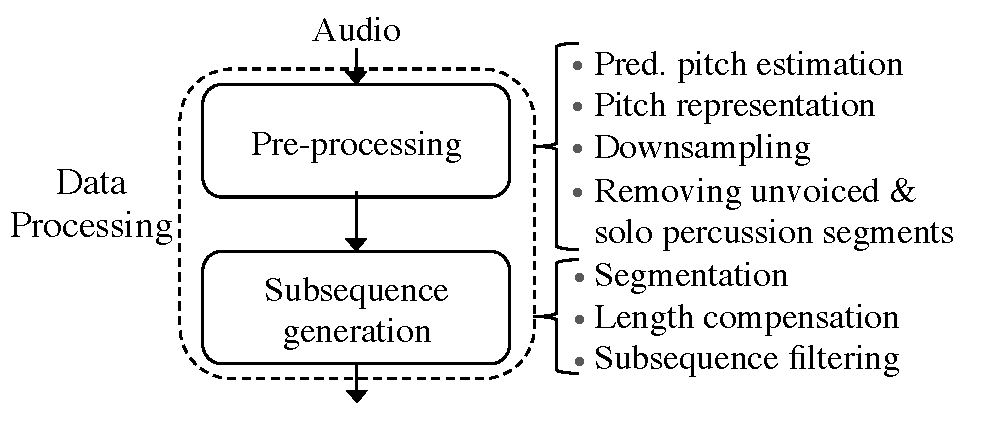
\includegraphics[width=\figSizeEightyFive]{ch06_patterns/figures/discovery/blockDiagram_DataProc.pdf}
	\end{center}
	\caption[Block diagram of data processing modules for melodic pattern discovery]{Block diagram of the data processing block in melodic pattern discovery task.}
	\label{fig:pattern_discovery_preprocessing_block_diagram}
\end{figure}


The steps involved in the pre-processing block are shown in Fig.~\ref{fig:pattern_discovery_preprocessing_block_diagram}. A description of each of these steps is given below:

\paragraph{a) Predominant Pitch Estimation and Representation} 

We consider melody as the predominant pitch in the audio signal. For estimating predominant pitch we follow the procedure we used in~\secref{sec:patterns_evaluation_of_similarity_measures}, which is described in detail in~\secref{sec:data_preprocessing_predominant_melody_estimation}. We use a frame size of 46\,ms and a hop size of 4.44\,ms. Noticeably, the predominant pitch estimation method that we use also performs voicing detection, which is used in the later part of our data processing methodology to filter unvoiced segments (\figref{fig:pattern_discovery_preprocessing_block_diagram}). We do not perform any post-processing on the estimated pitch contours.

For the melody representation to be musically relevant, the pitch values are converted from Hertz to Cents (\secref{sec:data_processing_cent_conversion}). In order to compare melodies across different artists and recordings we additionally consider the tonic pitch of the lead artist in the recording as the reference frequency during this conversion. The tonic of the lead artist for each recording in the collection is identified automatically using \acrshort{tonicid_justin} method, which is found to be the best performing method for this task in our comparative evaluation~(\secref{sec:data_preprocessing_tonic_identification}).

In the new variant of our method we post-process the predominant pitch contours as described in~\secref{sec:data_preprocessing_pitch_postprocessing}. We perform median and Gaussian filtering to remove spurious pitch jumps lasting over a few samples and to smooth the pitch contours. In addition, we also interpolate short non-voiced segments that usually correspond to intra-phrase breath pauses or to consonants in the lyrics (\secref{sec:data_processing_pitch_interpolation}). 


\begin{figure}
	\begin{center}
		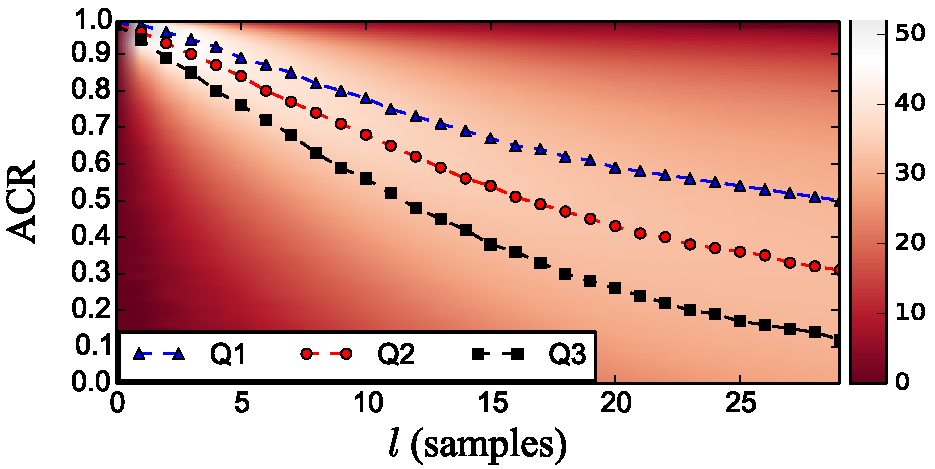
\includegraphics[width=\figSizeEightyFive]{ch06_patterns/figures/discovery/ACRHistogram.pdf}
	\end{center}
	\caption[Histograms of autocorrelation of the pitch subsequences for different lags]{Histograms of \gls{acr} values (histogram value is indicated by the colormap on the right: for ease of visualization, we compress the range of the histogram values by taking its fourth root). Q1, Q2 and Q3 denote the three quartile boundaries of the histogram. }
	\label{fig:ACRHistogram}
\end{figure}


\paragraph{b) Downsampling} 
As mentioned above, we estimate predominant pitch at a sampling rate of around 225\,Hz. However, in order to reduce the computational cost, we downsample the predominant pitch sequence~(\figref{fig:pattern_discovery_preprocessing_block_diagram}). We could not find any study that systematically reports the effect of sampling rate on melodic similarity in \gls{iam}\footnote{Note that the current study was performed before our supervised studies presented in~\secref{sec:patterns_evaluation_of_similarity_measures} and \secref{sec:patterns_improving_melodic_similarity}, where we analyse the influence of sampling rate on melodic similarity.}. In such a case, we derive an optimal sampling rate by analyzing the \gls{acr} of short-time pitch segments generated using a sliding window of 2\,s. We compute the \gls{acr} of all possible pitch segments in the entire dataset for different lags $l$, $l\in \lbrace0,1,\dots30\rbrace$, and examine the histogram of normalized \gls{acr} values at each lag (\figref{fig:ACRHistogram}). We select the lag at which the third quartile Q3 has an \gls{acr} value of 0.8, which corresponds to a sampling rate of 22.22\,ms~(or 45\,Hz). We informally found that this sampling rate generally preserves melodic nuances and rapid pitch movements in Carnatic music while reducing the computational requirements of the task. Note that in the new variant of our method, we use the optimal sampling rate derived from our comprehensive quantitative evaluations in~\cite{gulati_ICASSP2015} (see~\secref{sec:patterns_evaluation_of_similarity_measures}). %We use a sampling rate of 56\,Hz for Carnatic music and 45\,Hz for Hindustani music. 


%Note that the study in this section was originally presented in~\cite{gulati_SITIS_2014} and was conducted before we quantitatively assessed the optimal parameter settings in~\cite{gulati_ICASSP2015} (see~\secref{sec:patterns_evaluation_of_similarity_measures}). In the subsequent studies Although, the heuristically chosen sampling rate in this study is not drastically different from the optimal sampling rate reported in~\cite{gulati_ICASSP2015} (see \TODO{Figure(where we show the accuracy vs sampling rate)}). 


\paragraph{c) Solo Percussion Removal} 

As described in \secref{sec:pre_processing_tani_segmentation}, a concert of Carnatic music typically contains a solo percussion section, referred to as a \gls{tani} section, which can last up to 2-25\,minutes. We find that the predominant pitch estimation method employed in this study often tracks pitch corresponding to the \gls{mridangam} strokes instead of detecting \gls{tani} sections as non-voiced segments. This poses a challenge for melodic pattern discovery as there are several repeating percussion patterns in \gls{tani} sections, which are often discovered as the closest melodic pattern pairs. In \secref{sec:pre_processing_tani_segmentation}, we explain this issue in detail and describe a classification-based approach to detect \gls{tani} sections in audio recordings of Carnatic music. Once detected, we can simply discard the pitch samples corresponding to these sections and overcome the challenge. In addition to avoiding the unwanted melodic patterns being present in the output, by discarding the \gls{tani} sections we also reduce the computational complexity of our method.


\subsubsection{Subsequence Generation}
\label{sec:subsequencegeneration}

In this processing block we generate melodic pattern candidates from the resultant pitch representation~(\figref{fig:pattern_discovery_preprocessing_block_diagram}). The steps involved in generating candidate subsequences are described below.

\paragraph{a) Segmentation} 

As seen in~\secref{sec:patterns_melodic_similarity_results_discussions}, an accurate segmentation of melodic patterns has a big impact on the computation of melodic similarity, and eventually on the retrieval accuracy of melodic patterns. In the literature (\secref{sec:motif_in_symbolic_music}) there are several models studied for melodic segmentation~\citep{Cambouropoulos2006,muller2009robust,cambouropoulos2001local}. \cite{pearce2008comparison} and \cite{rodriguez2014comparing} provide a comparison of a number of such models. However, none of these models is directly applicable on the continuous melody representation we use for \gls{iam}. Due to the lack of such studies and reliable models for segmentation of melodic patterns in \gls{iam}, we use a brute-force approach for generating pattern candidates. We generate candidate pitch subsequences by using a sliding window of length $\pattLenSec$ with a hop size of one sample. Given no quantitative studies investigating the length of the melodic patterns in \gls{iam}, we make a choice of $\pattLenSec = 2$\,s based on recommendations from a few professional musicians.

Since unvoiced segments are removed from the pitch sequence at the pre-processing step~(\figref{fig:pattern_discovery_preprocessing_block_diagram}), a pattern candidate can include pitch samples separated by more than $\pattLenSec$ seconds. To handle these cases, we use the time stamps of the first sample ($\timeStamp_1$) and the last sample ($\timeStamp_2$) in the subsequence. We filter out all subsequences for which $\timeStamp_2-\timeStamp_1 > \pattLenSec + \shortPauseDur$. We select $\shortPauseDur =0.5$\,s to account for the short pauses during a phrase rendition. This value was empirically set to differentiate between inter- and intra-phrase pauses. 

In the new variant of our method, the processing step described in the previous paragraph becomes redundant, and is therefore not applied. Since in this variant the short-duration unvoiced regions in the predominant pitch contours are interpolated, there will not be any situation where $\timeStamp_2-\timeStamp_1 > \pattLenSec + \shortPauseDur$. 


\paragraph{b) Subsequence Filtering} 

One of the challenges in melodic pattern discovery is the presence of combinatorial redundancy in the form of musically trivial patterns in the output~\citep{Lartillot2005}. One such redundancy in our case is that of a melodic pattern comprising a single \gls{svara}. Instead of removing such musically uninteresting patterns after they are discovered, we detect and discard such subsequences (or pattern candidates) during the pre-processing step (\figref{fig:pattern_discovery_preprocessing_block_diagram}). The criterion for discarding such subsequences is summarized below:
\begin{equation}
\label{eq:flatness_measure}
\flatMeas =\sum_{i=0}^{\pattLenSym} \heaviside\left(\stdDevSubSeq_i\geq \stdDevThsld\right),
\end{equation}
\noindent where $\flatMeas$ is the flatness measure of a subsequence, $\pattLenSym$ denotes its number of samples, $\heaviside(z)$ is a Heaviside step function yielding $\heaviside(\text{true})\!=\!1$ and $\heaviside(\text{false})\!=\!0$, and $\stdDevSubSeq_i$ is the standard deviation at the $i$-th sample of a subsequence, computed using a window of length $\stdDevWin$ centered at sample $i$. The threshold $\stdDevThsld$ determines if a sample belongs to a flat region or not. In order to determine the optimal values of $\stdDevWin$ and $\stdDevThsld$, we manually labeled a number of regions in pitch contour as `flat' and `non-flat' for 4 excerpts in our database. We iterated over different parameter values and analysed the resultant \acrshort{roc} curve shown in~\figref{fig:ROC_pattern_discovery}). %In we show the ROC curve obtained for $\stdDevWin \in \lbrace100,200,400\rbrace$\,ms. 
Doing so, we found that $\stdDevWin=200$\,ms resulted in the best performance and that the knee of the curve corresponded to $\stdDevThsld=45$\,Cents. Having a value of $\flatMeas$ for each subsequence, we finally filter out the ones for which $\flatMeas \leq \flatThsld \pattLenSym$, using $\flatThsld = 0.8$. The latter was set by visual inspection.

\begin{figure}
	\begin{center}
		\ifdefined\PRINTVER
			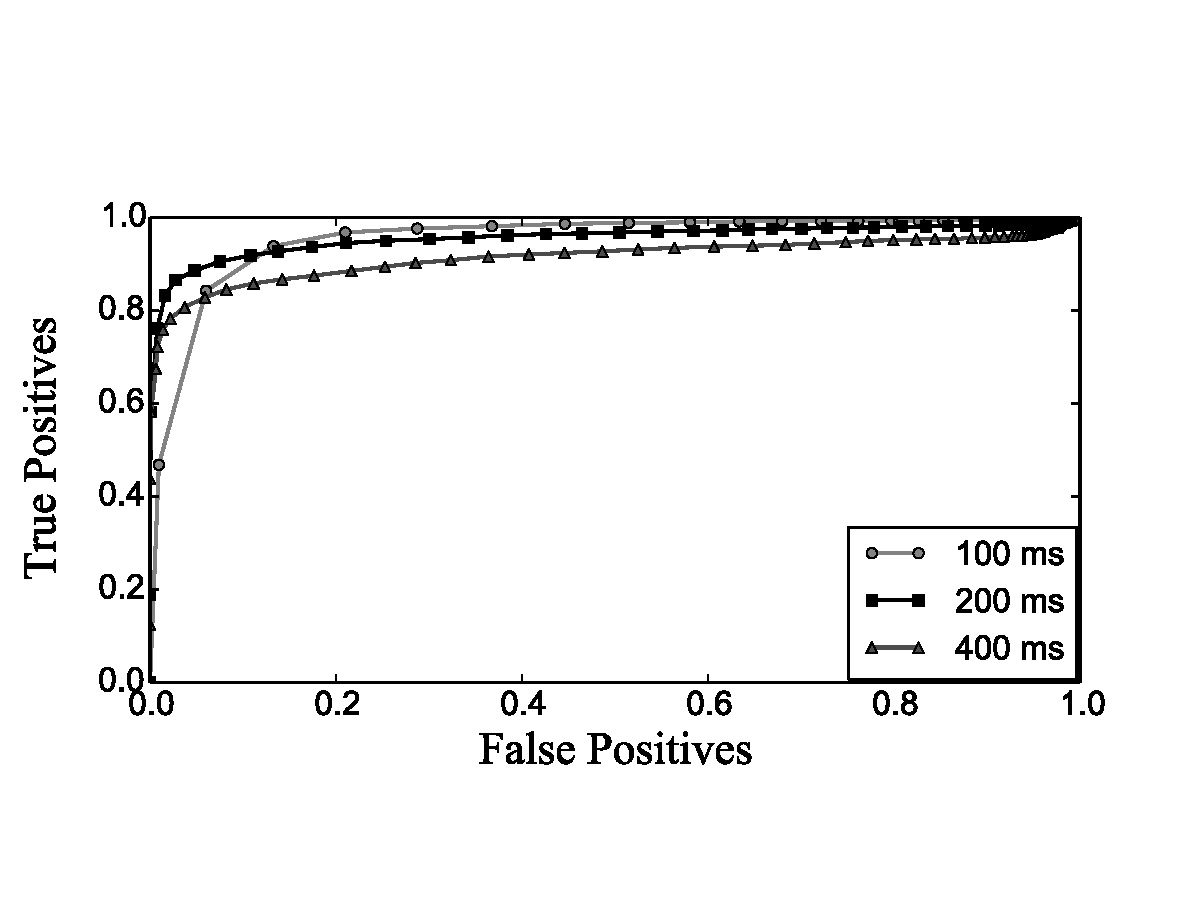
\includegraphics[width=\figSizeSeventy]{ch06_patterns/figures/discovery/ROCFlatness_BW.pdf}
		\else
			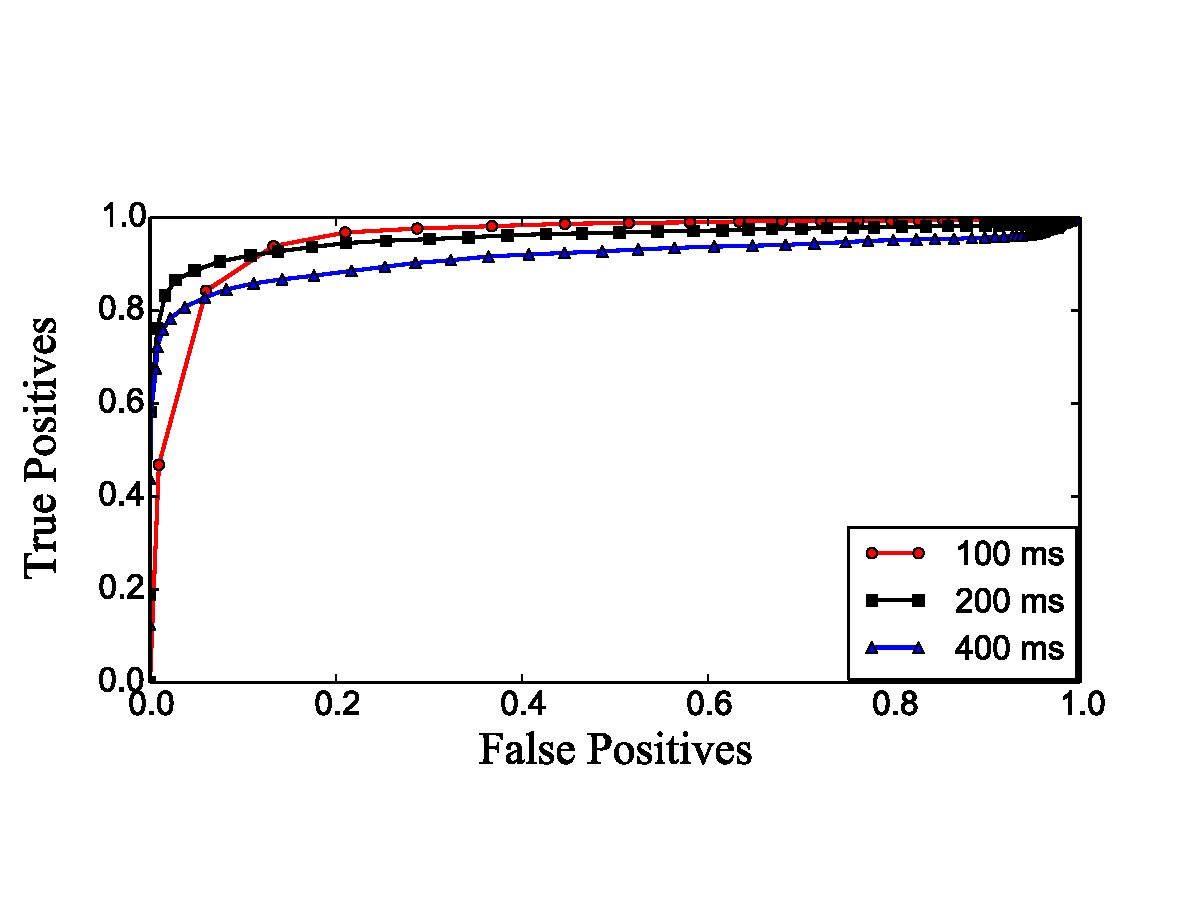
\includegraphics[width=\figSizeSeventy]{ch06_patterns/figures/discovery/ROCFlatness.pdf}
		\fi
	\end{center}
	\caption[\acrshort{roc} curve for `flat' and `non-flat' region classification]{\acrshort{roc} curves for `flat' and `non-flat' region classification for different values of window length ($\stdDevWin$) used for selecting an optimal value of the standard deviation.}
	\label{fig:ROC_pattern_discovery}
\end{figure}

In the new variant of our pattern discovery method, we use the segmentation approach described in~\secref{sec:nyas_svara_segmentation_method} to detect the stable \gls{svara} regions in melodies. The pitch samples in a subsequence that correspond to these stable \gls{svara} regions are regarded as `flat', which is analogous to $\stdDevSubSeq_i\geq \stdDevThsld$ being `True' for those samples. All other parameters remain the same as described above. This change is done because the segmentation approach produces more reliable estimates of the stable melodic regions compared to the simple measure using local standard deviation of the pitch samples. 

 %In the current study our dataset comprises only Carnatic music. For Hindustani music the reduction ratio of number of pattern candidates might be even higher due to the presence of long held \gls{svaras}.

\subsubsection{Intra-recording Pattern Discovery}
\label{sec:intraRecordingPatternDiscovery}

In this step our aim is to discover melodic patterns within each recording in the audio collection. We perform an exact pattern discovery by computing the similarity between every possible subsequence pair obtained within an audio recording. Thus, the computational complexity of this task is quadratic ($\bigO(n^2)$) over the number of subsequences. We regard the top $\topKIntra=25$ closest subsequence pairs in each recording as seed patterns. We omit overlapping subsequences in order to avoid trivial matches and additionally constrain the top $\topKIntra$ seed pattern pairs to be mutually non-overlapping. Due to this constraint for some recordings we obtain less than 25 pattern pairs. 


\paragraph{Melodic Similarity} 

We compute melodic similarity between two subsequences using a \gls{dtw}-based distance measure (\secref{sec_DTW_distance_measure}). This choice is supported by our findings in~\secref{sec:patterns_melodic_similarity_results_discussions}, wherein we showed that a \gls{dtw}-based distance measure outperforms Euclidean distance measure in melodic similarity computation in \gls{iam}. We use a step condition of $\lbrace(1,0), (1,1), (0,1)\rbrace$ and the squared Euclidean distance as the cost function. The accumulated cost matrix for this step condition is computed as described in \eqnref{eq:dtw_classic_cost_matrix_computation}. We do not use any penalty for insertion and deletion. In addition, we apply the Sakoe-Chiba global constraint with the band width set to 10\% of the pattern length. This constraint was found to be sufficiently large for accounting time warpings in melodic repetitions in Carnatic music (see \tabref{tab:melodic_similarity_results}). For the case of Hindustani music, an unconstrained \gls{dtw} variant is shown to perform the best. However, to make the system computationally tractable we finally choose 10\% band width for both the music traditions. Notice that these parameter values are close to the optimal settings but not the most optimal settings for a \gls{dtw} variant that we obtained in \secref{tab:melodic_similarity_results}. We make these compromises in order to avail lower bounding techniques as explained in the subsequent sections. 	

\paragraph{Lower Bounding \gls{dtw}}
\label{LowerBoundingDTW}

The computational complexity of a brute-force pattern discovery system using a \gls{dtw} distance measure is quadratic ($\bigO(n^2)$) over both the number of subsequences and the length of a subsequence. For a dataset as big as ours that contains millions of subsequences (pattern candidates), where the length of each subsequence is around 100\,samples, the system becomes extremely demanding in terms of the CPU time. Even after reducing the number of pattern candidates by filtering out subsequences in the pre-processing step and reducing the length of the subsequences by downsampling the pitch representation, it is not practically feasible to perform the task. One of the ways to address this problem is to use indexing or lower bounding techniques with which we can prune subsequence pairs that can not possibly be the best matches. Pruning of the subsequence pairs reduces the number of times the \gls{dtw} computation is done, and thus make \gls{dtw} distance computations tractable for datasets with large number of subsequences.

In literature there are several methods proposed for indexing the \gls{dtw} distance~\citep{Keogh2004,vlachos2003indexing,kim2001index}. These methods differ in terms of their computational complexities and the type of indexing techniques they employ (approximate or exact). In this study to speed up \gls{dtw} computations we use the exact \gls{dtw} indexing technique~\citep{Keogh2004} and apply cascaded lower bounds as explained in~\cite{Rakthanmanon2013}. This method is parameter free, it does not require any pre-processing of the data and there is no constraint on the minimum and maximum query length. In particular, we use \acrshort{lbKIMFL} (first-last) lower bound~\citep{kim2001index} and \acrshort{lbKeogh} bound~\citep{Keogh2004} for both query to reference and reference to query matching (denoted by \acrshort{lbKeoghEQ} and \acrshort{lbKeoghEC}, respectively). In \acrshort{lbKeoghEQ} lower-bounding envelopes are computed for the query pattern, and in \acrshort{lbKeoghEC}, they are computed for the reference. Besides, we apply early abandoning, both during the computation of lower bounds as well as during the \gls{dtw} distance computation. These lower bounding techniques are explained in~\secref{sec:background_lowerbound}, however, for a more detailed explanation we refer to~\cite{Rakthanmanon2013}. 

In \algoref{alg:algorithmdiscovery} we show the pattern discovery routine that uses cascaded lower bounds to speed up \gls{dtw}. This pseudo-code provides a better understanding of the pruning procedure and puts in context the utility of using different lower bounds. Note that in this routine we show the discovery of only the closest subsequence pair. With a trivial addition of incorporating a priority queue that stores the K most closest subsequence pairs at each step, we extend it to our use-case of discovering the top K closest melodic patterns. We further optimize this routine by pre-computing the subsequence envelopes used in the computation of LB\_Keogh bound (\secref{sec:background_lowerbound}).

\renewcommand{\algorithmiccomment}[1]{\bgroup\hfill\tiny//~#1\egroup}
\begin{algorithm}
\caption{Discovering the closest subsequence pair using the \gls{dtw} distance and cascaded lower bounds.}
\label{alg:algorithmdiscovery}
	\begin{algorithmic} 
	
	\State {\bf Input:} array $\patternArray$ containing $N$ number of subsequences
	\State \texttt{best\_so\_far} = \texttt{infinity};
	\For{$i$=0; $i \leq N-1$; $i$++}
		\For{$j$=0; $j \leq N-1$; $j$++}
			\State  \texttt{dist\_FL} = \texttt{\acrshort{lbKIMFL}($\pattern_i$, $\pattern_j$)}			
			\If {\texttt{dist\_FL} < \texttt{best\_so\_far}}				
				\State  \texttt{dist\_EQ} = \texttt{LB\_Keogh($\pattern_i$, $\pattern_j$)}				
				\If {\texttt{dist\_EQ} < \texttt{best\_so\_far}}				
					\State  \texttt{dist\_EC} = \texttt{LB\_Keogh($\pattern_j$, $\pattern_i$)}					
					\If {\texttt{dist\_EC} < \texttt{best\_so\_far}}					
						\State  \texttt{true\_dist} = \texttt{DTW($\pattern_i$, $\pattern_j$)}						
						\If {\texttt{true\_dist} < \texttt{best\_so\_far}}
							\State \texttt{best\_so\_far} = \texttt{true\_dist}
							\State \texttt{closest\_pair\_index} = ($i$,$j$)							
						\EndIf
					\EndIf
				\EndIf
			\EndIf
		\EndFor
	\EndFor
	
	\end{algorithmic}
\end{algorithm}
				

\paragraph{Pattern Length Compensation}
\label{PatternLengthCompensation}

Along with the local non-linear time warping, the overall length of a melodic pattern may also vary across repetitions. For example, a melodic pattern of length 2\,s might be sung in 2.2\,s in a different position in the recording. We handle this by using multiple time scaled versions of a subsequence in the distance computation. 
Performing appropriate uniform time-scaling prior to \gls{dtw} is known to produce tighter lower bounds~\citep{Zhu2003}, which is similar to a technique referred to as local \gls{dtw}. It should be noted that such timing variations could as well be addressed by using a subsequence variant of \gls{dtw}. However, the lower bounding techniques we use to speed up the \gls{dtw} distance computation do not work for the subsequence variant of the \gls{dtw}. 

For every subsequence, we generate five subsequences by uniformly time scaling it by a factor of $\timeScaFac \in \lbrace 0.9, 0.95, 1, 1.05, 1.1\rbrace$, such that the length of the resulting subsequences is $\pattLenSec$. We use cubic interpolation for uniformly time scaling a subsequence. Creating five uniform time scaled subsequences for each subsequence increases the computational cost by a factor of 25. We observe that the distance between a subsequence pair $X_{1.0}$ and $Y_{1.05}$ is very close to the distance between the pair $X_{1.05}$ and $Y_{1.1}$ (the sub-index denotes the interpolation factor $\timeScaFac$). Thus by following this rationale and using this approximation, we can avoid the distance computation between 16 of the 25 combinations without a significant compromise on accuracy. We only retain the combinations for which the difference between the interpolation factors of subsequence pairs are unique.

\subsubsection{Inter-recording Pattern Detection}
\label{sec:inter_recording_pattern_search}

After discovering melodic patterns within each audio recording, we now proceed to detect their occurrences in all the recordings in the collection. For this, we consider every seed pattern as a query and perform an exhaustive search over all the subsequences obtained from the entire audio music collection. For every seed pattern we store top $\topKInter=200$ closest matches (referred to as search patterns). To avoid redundancy in the search results, we constrain search patterns for every seed pattern to be mutually non-overlapping. Similar to the intra-recording pattern discovery step, here also for every subsequence we consider 5 uniformly time scaled subsequences in the distance computation. Furthermore, for detecting occurrences of seed patterns in other recordings we use the same similarity measure and lower bounding techniques as used in Intra-recording pattern discovery. The pattern detection routine is a small modification of the routine shown in~\algoref{alg:algorithmdiscovery}. Instead of a single subsequence array, we would have two arrays: one of which comprises the seed patterns (queries) and the other comprises subsequences obtained from all the recordings (target candidates). 

\subsubsection{Rank Refinement}
\label{sec:rankRefinement}

As mentioned before, the lower bounds used for speeding up the distance computations are not valid for any variant of the \gls{dtw} distance. This constraint governed the choices made for the \gls{dtw} variant and the parameter settings for computing melodic similarity in both the intra and the inter-recording pattern processing blocks. However, once the top matches are found, nothing prevents us from reordering the ranked list using any variant of the \gls{dtw} distance. This is because the number of top matches we consider ($\topKInter=200$) per query is orders of magnitude smaller than the total number of subsequences obtained from the entire audio collection. For every query pattern, we now recompute the melodic similarity with its top $\topKInter$ search patterns using a more robust and a better performing variant of the \gls{dtw} distance.

\begin{figure}
	\begin{center}
		\ifdefined\PRINTVER
			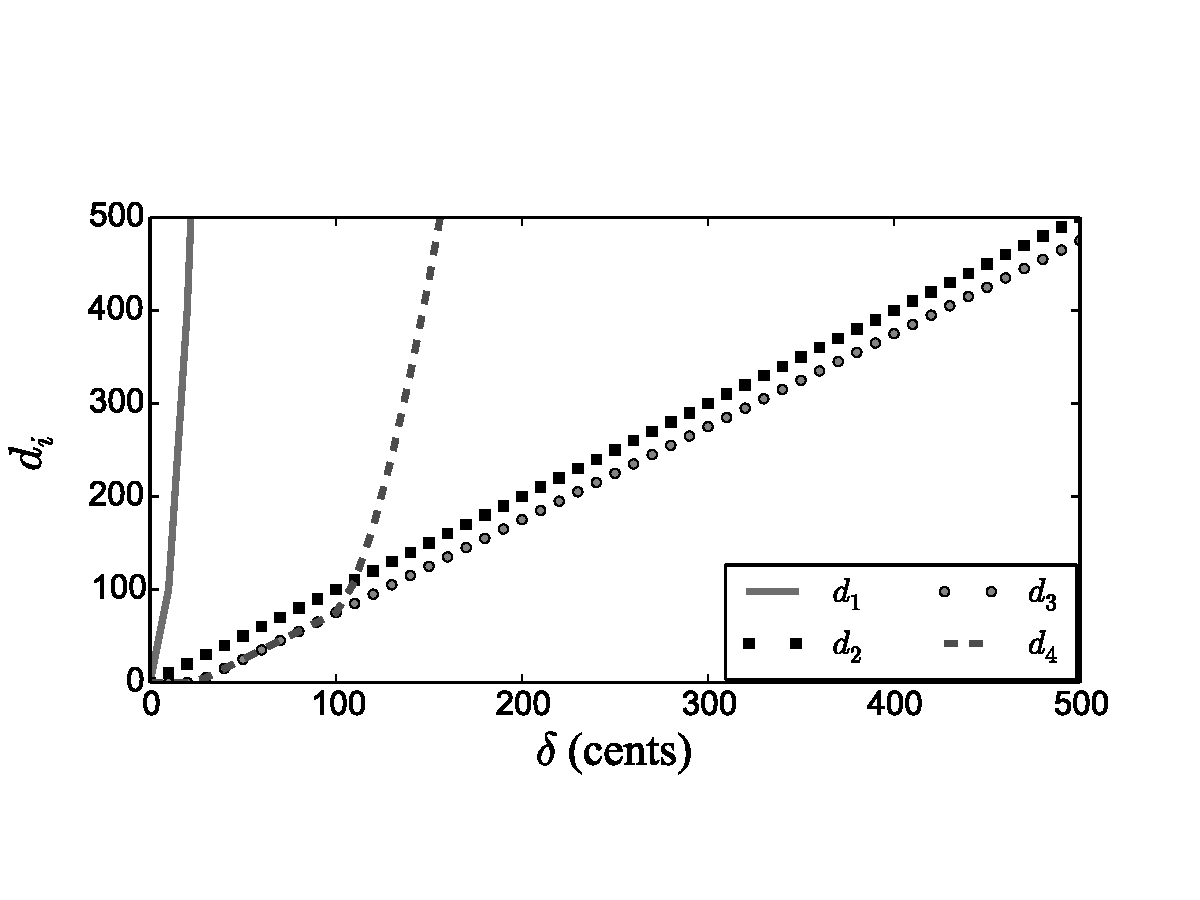
\includegraphics[width=\figSizeEighty]{ch06_patterns/figures/discovery/distances_BW.pdf}
		\else
			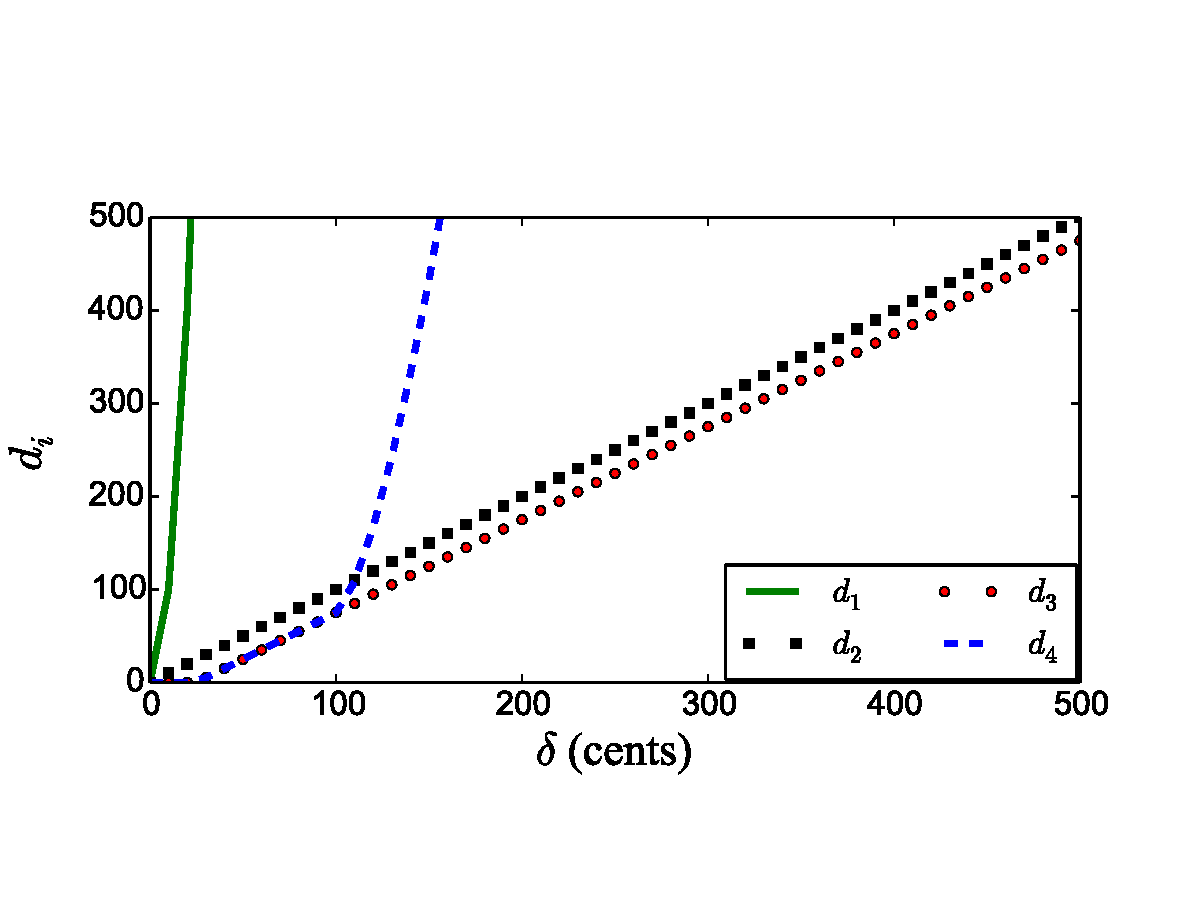
\includegraphics[width=\figSizeEighty]{ch06_patterns/figures/discovery/distances.pdf}
		\fi
	\end{center}
	\caption[Illustration of output of different distance measures]{Output of the four different distance measures ($\dtwCostFnc_i$, $i \in \lbrace 1\cdots4 \rbrace$) as a function of cityblock distance \pitchDiff.}
	\label{fig:Distances_DTW_discovery}
\end{figure}

During rank refinement, we select a \gls{dtw} step condition of $\lbrace(1,2), (1,1), (2,1)\rbrace$ to avoid some pathological warping of the path. This step condition, which also acts as a local constraint was shown to better model the melodic similarity in~\secref{sec:patterns_melodic_similarity_results_discussions}. Furthermore, we investigate four different distance measures $\dtwCostFnc_i$, $i=1,\dots 4$, used in the computation of the \gls{dtw} cost matrix. These distance measures are described below in~\eqnref{eq:distance_measures_discovery}. For a better understanding of the distance measures we also show them in~\figref{fig:Distances_DTW_discovery}.
\begin{equation}
\begin{aligned}
\dtwCostFnc_1& = \pitchDiff \hspace{.5em}\\
\dtwCostFnc_2& = \pitchDiff^2 \hspace{.5em}\\
\dtwCostFnc_3& = 
\begin{cases}
\pitchDiff-25, & \hspace{1cm} \text{if } \pitchDiff >25\\
0, & \hspace{1cm}\text{otherwise } 
\end{cases}\\
\dtwCostFnc_4 &= 
\begin{cases}
(\pitchDiff-\arbitTshldOne)^{1.5} + \arbitTshldTwo, & \text{if } \pitchDiff >100\\
\dtwCostFnc_3, & \text{otherwise}
\end{cases}
\end{aligned}
\label{eq:distance_measures_discovery}
\end{equation}

\noindent where $\pitchDiff = |\pitchCents_1-\pitchCents_2|$ is the city block distance between two pitch values and all numeric values are in Cent scale. We set $\arbitTshldOne =99.55$ and $\arbitTshldTwo = 74.7$ to maintain point and slope continuity of the function. The formulation for these different distance measures ($\dtwCostFnc_i$) is inspired by our own experience and some of the approaches we find in the literature~\citep{Ishwar2013,Rao2014}. We denote the four variants of the rank refinement method by $\RankRefVar_i$, where $i \in \lbrace 1\cdots4 \rbrace$.


\subsection{Evaluation}

\subsubsection{Music Collection}
\label{sec:pattern_discovery_musiccollection}

The music collection used for studying the task of pattern discovery in this section comprises 365\,hours Carnatic music. It contains 1764 audio recordings, which are carefully compiled as a part of the CompMusic Carnatic music corpus (\secref{sec:corpus_carnatic_music_corpus}). As explained in~\secref{sec:corpus_carnatic_music_corpus}, these audio recordings are ripped from commercially released music CDs. The selected music material is diverse in terms of the number of artists, gender of lead artists, number of different \glspl{raga}, year of release and various forms within Carnatic music.
%\COMMENT{If time permits provide statistics of this dataset here as well? they are already talked about in the corpus chapter}


\subsubsection{Evaluation Methodology}
\label{sec:evaluationmethodology}

One of the challenges in an unsupervised data-driven approach such as the one we use for discovering melodic patterns is its evaluation. We here perform a quantitative evaluation based on expert feedback. For the entire dataset we obtain over 15\,million search patterns for each of the rank refinement methods. We divide seed patterns into three categories based on the distance between the seed pairs, which we denote by $\distPatt$. The distribution of the distance $\distPatt$ between the seed pattern pairs is shown in~\figref{fig:SeedPatternsDistanceDistribution}. Then, to have an equal representation from the range of values of $\distPatt$, 200 seed pairs equally distributed among these categories are randomly selected for evaluation. Seed category boundaries are $\mu \pm 1.5\sigma$, where $\mu$ and $\sigma$ are the mean and the standard deviation of the distribution of $\distPatt$. For every selected seed pattern we consider the first 10 search patterns for each of the four rank refinement methods for evaluation. Thus, in total, we obtain 200 seed pairs and 8,000 search patterns for expert evaluation.

Expert evaluation is performed by a professional Carnatic musician who has received over 20 years of music education. For examining similarity between two melodic patterns, the musician listened to the audio fragments corresponding to these patterns and scored a 0 for melodically dissimilar and a 1 for melodically similar pattern. The musician annotated melodic similarity for each seed pair and between the seed and its search patterns for every rank refinement method.


\begin{figure}
	\begin{center}
		\ifdefined\PRINTVER
			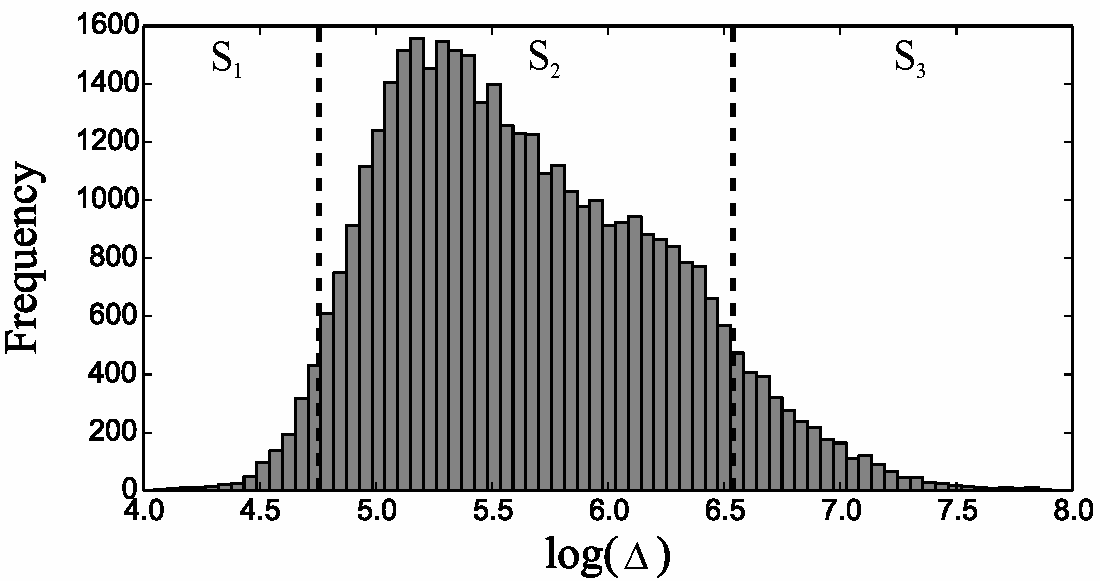
\includegraphics[width=\figSizeEightyFive]{ch06_patterns/figures/discovery/SeedDistribution_BW.pdf}
		\else
			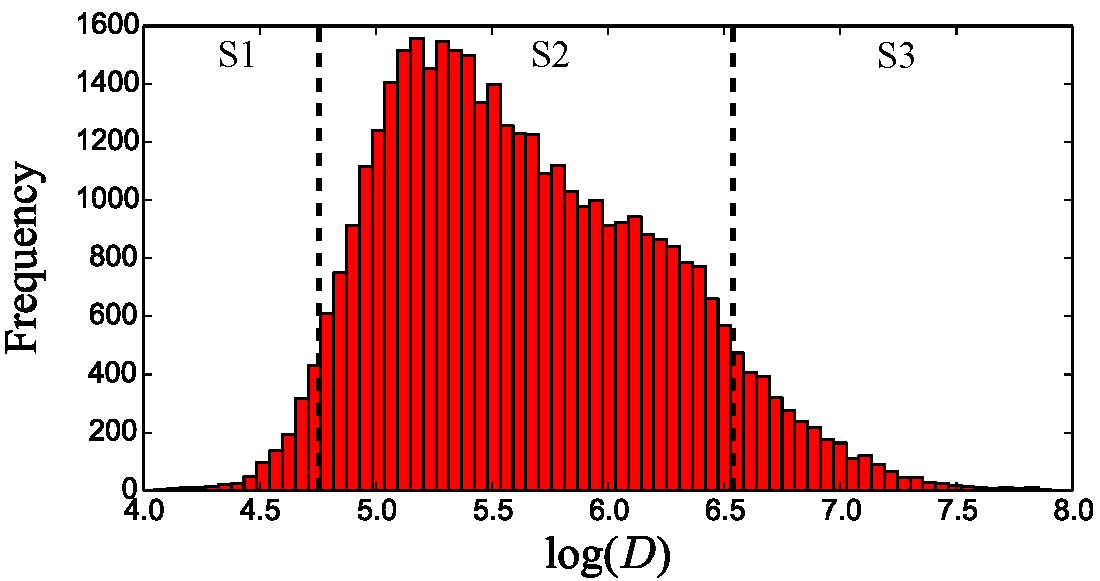
\includegraphics[width=\figSizeEightyFive]{ch06_patterns/figures/discovery/SeedDistribution.pdf}
		\fi
	\end{center}
	\caption[Distance distribution of seed melodic patterns]{Distance distribution of seed patterns. Three seed pattern categories are marked by $\seedPattCat_1$, $\seedPattCat_2$ and $\seedPattCat_3$.}
	\label{fig:SeedPatternsDistanceDistribution}
\end{figure}


To quantify the musician's assessment of the similarity between the melodic patterns we use \gls{map}, a typical evaluation measure in information retrieval~\citep{manning2008introduction}, which is also very common in \gls{mir}. This way, we have a single number to evaluate the performance of the four different rank refinement methods. Since we do not have ground-truth annotations of melodic patterns for our dataset, total number of occurrences of different patterns is unknown. Therefore, while computing the \gls{map} scores we consider the total number of relevant patterns as the number of relevant patterns retrieved in the top 10 search results. For assessing statistical significance we use the Mann-Whitney U test~\citep{mann1947test} with $\pVal < 0.05$. To compensate for multiple comparisons, we apply the Holm-Bonferroni method~\citep{holm1979simple}. Thus, eventually we use a much more stringent criterion than $\pVal < 0.05$ for measuring statistical significance. We also use \acrshort{roc} curves to analyse the separation between the distance distribution of melodically similar and dissimilar subsequences~\citep{manning2008introduction}. 


\subsection{Results and Discussion}
\label{sec:patterns_discovery_results}

Before presenting the results of the evaluation of the discovered patterns, we provide details in terms of the number of patterns and \gls{dtw} computations done at each step. Our dataset comprising 365\,hours of audio data contains nearly 300\,million pitch samples (considering 225\,Hz as the sampling rate of the pitch contours). In a brute force segmentation scenario that would amount to roughly the same number of pattern candidates. However, since we downsample the pitch contours and filter out musically trivial patterns, we retain around 17.5\,million pattern candidates after data pre-processing step. In the intra-recording pattern discovery block, for all the recordings, nearly 1.41\,trillion distance computations are done to obtain 79,172 seed patterns. In the inter-recording pattern detection block, nearly 12.42\,trillion distance computations are done to obtain 15 million search patterns for each variant of the rank-refinement method. These numbers give us an idea about the computational complexity of the task and shows the scale at which this study is performed.

\begin{table} 
	\begin{centering}
		\begin{tabular}{ c | c c }
			\tabletop
			Lower bound   	& Intra-rec.(\%)		&	Inter-rec.(\%) \\	
			\tablemid
			\acrshort{lbKIMFL}   	& 52	&	45 \\	
			\acrshort{lbKeoghEQ}   	& 23	&	51 \\
			\acrshort{lbKeoghEC}   		& 1	&	3 \\
			\tablebot
		\end{tabular}
		\caption[Percentage of exits after different lower bound computations]{Percentage of exits after a lower bound computation with respect to the total number of distance computations.}
		\label{tab:computationalStats}	
		\par \end{centering}	
\end{table}

We now analyse the contribution of different lower bounds in pruning the search space. In~\tabref{tab:computationalStats} we show in percentage the number of times the program counter exits after a lower bound computation with respect to the total number of distance computations. As mentioned before, the total number of distance computations are 1.41\,trillion for intra-recording pattern discovery and 12.42\,trillion for inter-recording pattern detection. From~\tabref{tab:computationalStats} we see that the \gls{dtw} computation is avoided in 76\% and 99\% of the distance computations done in the intra-recording pattern discovery and the inter-recording pattern detection task, respectively. It is evident that the lower bounding methods are more effective in the latter case compared to the former. This is expected as different songs may correspond to different \glspl{raga} and hence use different set of musical notes, which eventually produces tighter lower bounds. An interesting observation here is that \acrshort{lbKIMFL} lower bound whose computational complexity is $\bigO(1)$ prunes nearly 50\% of the total numbers of possible subsequence pairs. 

We now present our formal evaluations. We first evaluate the performance of the intra-recording pattern discovery task. We find that the fraction of melodically similar seed pairs within each seed category $\seedPattCat_1$, $\seedPattCat_2$ and $\seedPattCat_3$ consistently decreases: 0.98, 0.67 and 0.31, respectively. This is expected as the seed categories are created based on the distance ($\distPatt$) between the seed pairs. These numbers indicate that the computed distance strongly correlates to the melodic similarity between the patterns. However, from these numbers we do not get much information about the amount of separation between the distance distributions of melodically similar and dissimilar seed pattern pairs. To examine the separation, we compute the \acrshort{roc} curve as shown in~\figref{fig:combinedROCPatternDiscovery} (solid blue line). The knee of the curve corresponds to a precision of approximately 80\% for 10\% of false positive cases. This indicates that the chosen \gls{dtw}-based distance measure is a sufficiently good candidate for computing melodic similarity for the case of intra-recording seed pattern discovery. 


\begin{figure}
	\begin{center}
		\ifdefined\PRINTVER
			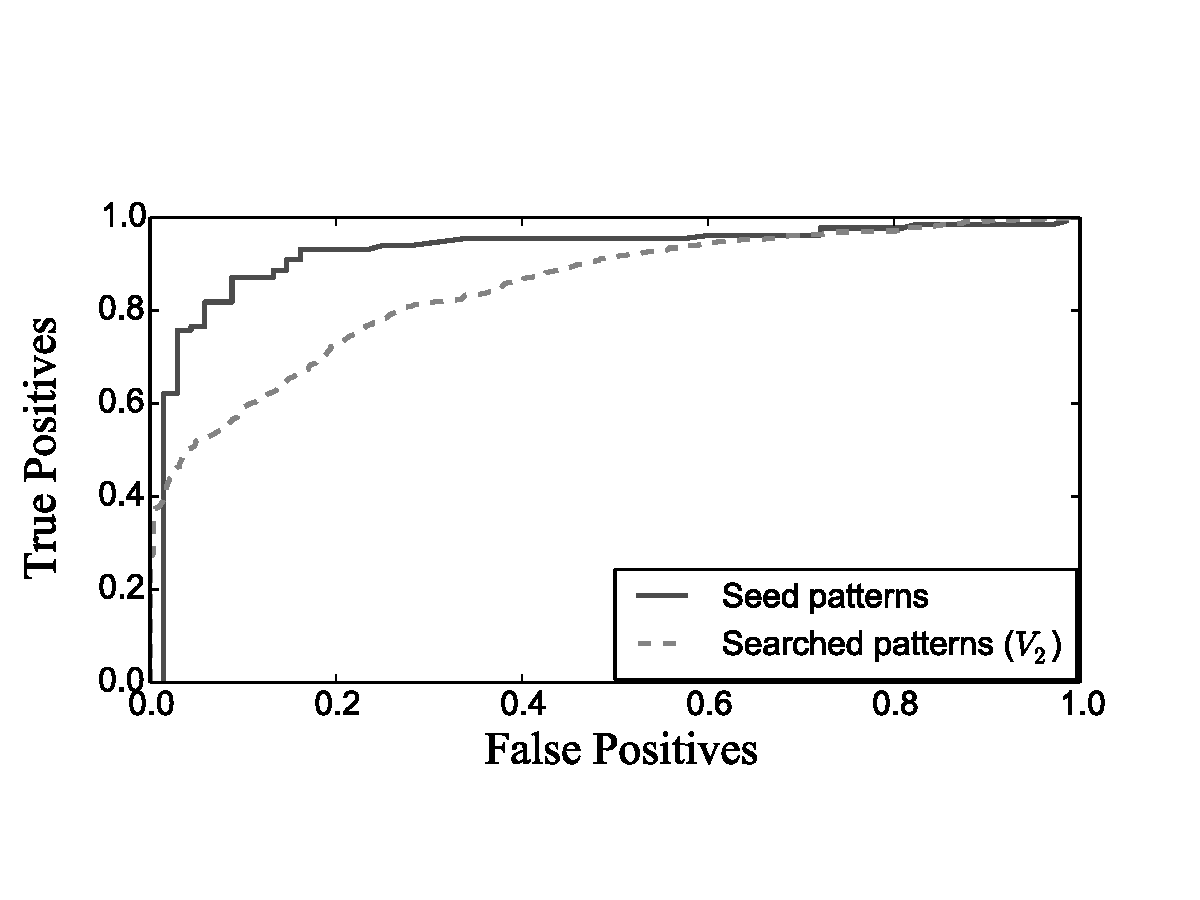
\includegraphics[width=\figSizeSeventy]{ch06_patterns/figures/discovery/seedROC_BW.pdf}
		\else
			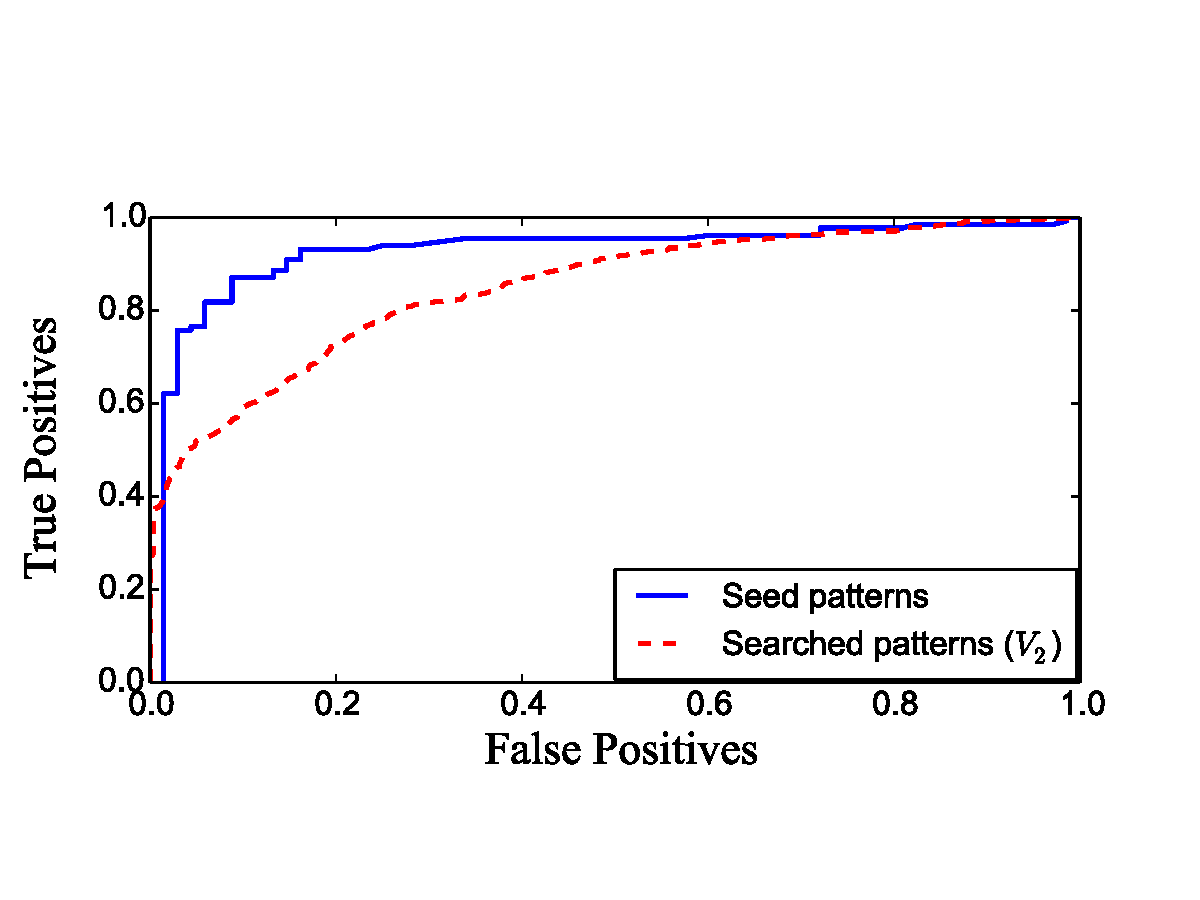
\includegraphics[width=\figSizeSeventy]{ch06_patterns/figures/discovery/seedROC.pdf}
		\fi
	\end{center}
	\caption[\acrshort{roc} curve for seed pairs and search patterns]{\acrshort{roc} curve for seed pairs and search patterns (using $\RankRefVar_2$) in the evaluation set.}%\vspace{-1em}
	\label{fig:combinedROCPatternDiscovery}
\end{figure}


\begin{table} 
	\begin{centering}	
		\begin{tabular}{ c | c c c c}
			\tabletop
			Seed Category   & $\RankRefVar_1$		&	$\RankRefVar_2$ & $\RankRefVar_3$	 &	$\RankRefVar_4$ 	\\	
			\tablemid
			$\seedPattCat_1$ & 0.92    &	0.92		&	0.91    &	0.89\\
			$\seedPattCat_2$ & 0.68    &	0.73		&	0.73    &	0.66\\
			$\seedPattCat_3$ & 0.35    &	0.34    &	0.35    &	0.35\\
			\tablebot
		\end{tabular}
		\caption[\acrshort{map} scores for four variants of rank refinement method for each seed pattern category]{\acrshort{map} scores for four variants of rank refinement method ($\RankRefVar_i$) for each seed category ($\seedPattCat_1$, $\seedPattCat_2$ and $\seedPattCat_3$).}
		\label{tab:meanAveragePrecision_pattern_discovery}
		\par \end{centering}	
\end{table}

Next, we evaluate the performance of inter-recording pattern detection task and assess the effect of the four \gls{dtw} cost variants explained in~\secref{sec:patterns_discovery_results} (denoted by $\RankRefVar_1 \dots \RankRefVar_4$). To investigate the dependence of the performance on the category of the seed pair, we perform the evaluation within each seed category. In~\tabref{tab:meanAveragePrecision_pattern_discovery} we show the \gls{map} scores obtained for the different variants of the rank refinement method ($\RankRefVar_1, \RankRefVar_2, \RankRefVar_3$ and $\RankRefVar_4$) for each seed category ($\seedPattCat_1$, $\seedPattCat_2$ and $\seedPattCat_3$). In addition, we also present a box plot of corresponding average precision values in~\figref{fig:boxPlotMAPPatternDiscovery}. In general, we observe that every method performs well for category $\seedPattCat_1$, with a \gls{map} score around 0.9 and no statistically significant difference between each other. For category $\seedPattCat_2$, $\RankRefVar_2$ and $\RankRefVar_3$ perform better than the rest and the difference is found to be statistically significant. The performance is poor for the third category $\seedPattCat_3$ for every variant. The difference in performance between any two methods across seed categories is statistically significant. We observe that \gls{map} scores across different seed categories correlate strongly with the fraction of melodically similar seed pairs in that category (discussed above). This means that the seed pattern pairs that have high distance $\distPatt$ between them obtain low average precision when used as query patterns and vice-versa. This might be because across repetitions of such patterns there could be a high degree of melodic variation, to model which the current similarity measure appears inadequate. In addition, closely repeating seed pattern pairs (i.e.~with low distance $\distPatt$ between them) might have more number of repetitions with low degree of melodic variations, for which the current similarity measure performs well. 

\begin{figure}
	\begin{center}
		\ifdefined\PRINTVER
			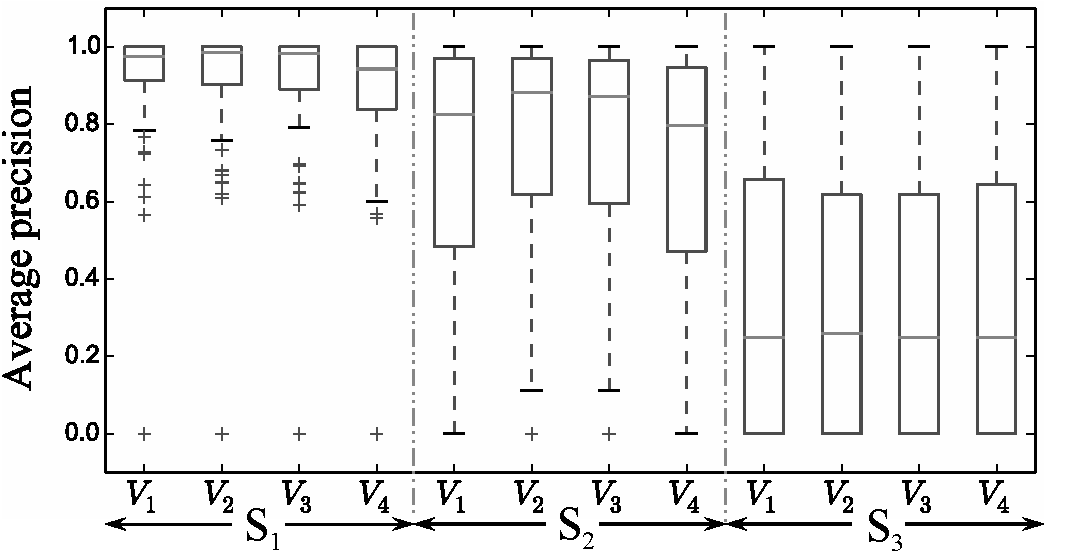
\includegraphics[width=\figSizeNinety]{ch06_patterns/figures/discovery/boxPlot_BW.pdf}
		\else
			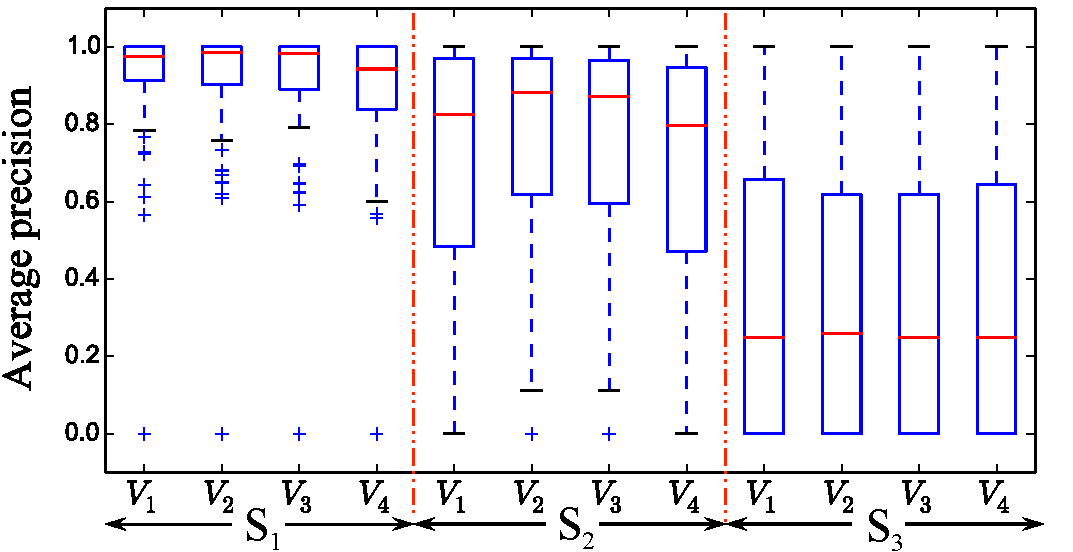
\includegraphics[width=\figSizeNinety]{ch06_patterns/figures/discovery/boxPlot.pdf}
		\fi
	\end{center}
	\caption[Boxplot of average precision values for the different variants of the rank refinement method]{Boxplot of average precision values for the different variants of the rank refinement method ($\RankRefVar_i$) for each seed category.}
	\label{fig:boxPlotMAPPatternDiscovery}
\end{figure}

%It suggests that repeating patterns do have some significance, they are not a product of coincidence, and therefore, they are more likely to recur across recordings. Note that we do not imply that every repeating pattern is (equally) musically significant or is a characteristic phrase of a \gls{raga}. There are different types of repeating patterns in melodies of \gls{iam}. The task of characterizing the discovered patterns is addressed in~\secref{sec:patterns_characterization_of_melodic_patterns} \TODO{rehphrase this last part}

Finally, we analyse the distance distributions of melodically similar and dissimilar search patterns. For this we use the best performing rank-refinement variant $\RankRefVar_2$. To examine the separation in the distance distribution, we compute the \acrshort{roc} curve as shown in~\ref{fig:combinedROCPatternDiscovery} (dashed red line). We observe that the separability between melodically similar and dissimilar subsequences in this case is poorer than the one obtained for the seed pairs (solid blue line). This suggests that it is much harder to differentiate melodically similar from dissimilar patterns when the search is performed across recordings. This can be attributed to the total number of melodically dissimilar subsequences (irrelevant documents) for every query subsequence, which is orders of magnitude higher in this task compared to the task of pattern discovery within a recording. In addition, one of the reasons can also be that the melodic phrases of two allied \glspl{raga} (\secref{sec:melody_in_iam}) are differentiated based on subtle melodic nuances~\citep{Viswanathan2004}. Hence, one faces a much more difficult task, which requires a superior melodic similarity measure.% Moreover, some of these melodic nuances might be specific to \glspl{raga}, learning which might be possible only under a supervised framework. 

To demonstrate the capabilities of the approach, we show a few examples of the discovered melodic patterns in~\figref{fig:combinedPatternsDiscovered}. Our approach robustly extracts patterns in different scenarios such as large local time warpings~(b), uniform scaling~(c), patterns with silence regions~(d) and across different tonic pitches~(e and f). It is worth mentioning that, during the process of annotation, the musician found several musically interesting results. For example, striking similarity between phrases of two different \glspl{raga}, between phrases in sung melodies and the melodies played on instruments (Violin or \Gls{vina}), and phrases sung by different artists. Many of the discovered patterns are the characteristic melodic phrases of the \glspl{raga}, which are the primary cues for \gls{raga} recognition. All the discovered melodic patterns in this study can be browsed and listened to through a web interface (\appref{app:resources}). Overall, we find that the obtained results are musically relevant and can be used to establish meaningful relationships between audio recordings. We explore the usability of these discovered patterns in the task of automatic \gls{raga} recognition in~\chapref{chap:raga_recognition}.
\begin{figure}
	\begin{center}
		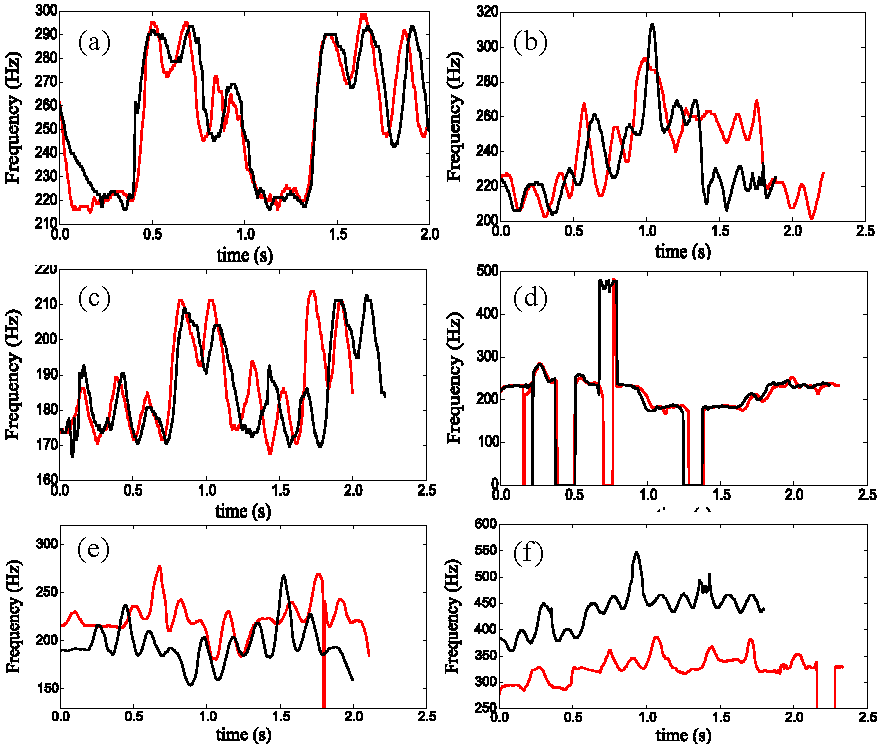
\includegraphics[width=\figSizeHundred]{ch06_patterns/figures/discovery/combinedPatterns.pdf}
	\end{center}
	\caption{Examples of the discovered melodic patterns.}
	\label{fig:combinedPatternsDiscovered}
\end{figure}

%################################################################################################################
%########################################### IMPROVING MELODIC SIMILARITY #######################################
%################################################################################################################


\section{Characterization of Melodic Patterns}
\label{sec:patterns_characterization_of_melodic_patterns}

In the previous section we described our approach to discover melodic patterns in sizable audio music collections of \gls{iam}. Our primary goal was to extract as many different types of repeating melodic patterns and as many occurrences of them as possible, irrespective of their musical relevance\footnote{Note that in our method in~\secref{sec:patterns_melodic_pattern_discovery}, we only removed melodically trivial patterns that comprise primarily single \gls{svara}.}. A well known problem with the computational approaches for musical pattern discovery is the large volume of discovered patterns, wherein a large fraction of them often tends to be musically uninteresting and irrelevant (\secref{sec:pattern_processin_in_music}). This aspect of automated methods for motivic analysis is studied by~\cite{marsden2012counselling}, who says:
\blockquote{\textit{...computational approaches find many more motives and many more relationships between fragments than in traditional motivic analysis...these are then filtered by some mechanism which selects motives and relationships with privileged positions within the network of relationships.}}

Thus, one of the main challenges of pattern discovery methods is to identify the musically meaningful patterns in the output. In the case of melodies in \gls{iam} as well recurring patterns differ drastically in terms of their musical relevance (\secref{sec:melody_in_iam}). Their functional role in melodies varies from being a melodic ornamentation to being a characteristic melodic phrase of a \gls{raga}. Thus, in order to effectively utilize the discovered melodic patterns in different melodic analyses and applications in \gls{iam}, characterization of these patterns in terms of their musical relevance and functional roles is crucial. In this section we address this issue and characterize discovered melodic patterns in order to identify one of the most interesting types of melodic patterns in \gls{iam}, the \gls{raga} motifs.
 
From the literature we see that most of the motivic analysis approaches employ a filtering step to select the musically significant patterns (\secref{sec:motif_in_symbolic_music}). A common approach is to prefer long duration patterns~\citep{Cambouropoulos2006,Karydis2006}. Another type of approaches prefer patterns that occur more frequently than others~\citep{Cambouropoulos2006,meredith2002algorithms}. The methods proposed by~\cite{conklin2010discovery,conklin2011comparative} are also based on patterns' frequency of occurrence, but inversely weighted by its frequency of occurrence in an anti-corpus. \cite{collins2011modeling} evaluate several strategies for assigning importance to discovered melodic patterns. A more detailed description of these filtering strategies is provided in~{\secref{sec:motif_in_symbolic_music}. We note that most of these filtering strategies are not directly applicable in our context. For example, since our discovery method operates with a limitation of a fixed length melodic pattern, the strategy of maximal length patterns is not applicable. The other type of commonly used strategy in which the most frequently occurring patterns are selected also appears futile. This is because in \gls{iam} \glspl{gamaka} and several other melodic ornaments are often the most frequently occurring patterns, which in our task are relatively less musically relevant compared to the \gls{raga} motifs. Thus, there is a need for a novel filtering strategy that can characterize discovered melodic patterns in \gls{iam} and can identify the musically interesting ones such as \gls{raga} motifs.	

There is another challenge in dealing with an in-exact or approximate melodic pattern matching methodologies, which is that of determining a meaningful similarity threshold. It becomes an even bigger challenge in an unsupervised analysis, such as the case in our pattern discovery method. The discovery approach described in~\secref{sec:patterns_melodic_pattern_discovery} works with a fixed number of closest pattern matches irrespective of the absolute value of the melodic similarity. As a result of which the output of the pattern discovery approach may contain a large amount of music irrelevant or noisy matches. Although, as seen in~\secref{sec:patterns_discovery_results}, separation between the distance distributions of melodically similar an dissimilar patterns appears favorable (\figref{fig:combinedROCPatternDiscovery}), indicating that an optimal melodic similarity threshold can potentially remove the noisy matches with a reasonable accuracy. However, determining such a melodic similarity threshold is non-trivial.

In this section we address both the issues, determining a meaningful melodic similarity threshold, and characterizing discovered melodic patterns by performing a network analysis. We exploit the topological properties of the network to determine a similarity threshold. For characterizing patterns we first detect non-overlapping communities in the network and then characterize the communities by utilizing the related editorial metadata. As described in~\secref{sec:melody_in_iam}, repeating patterns in melodies of \gls{iam} can belong to varied categories. In order to reduce the complexity involved in identification and evaluation of different types of melodic patterns, we focus on \gls{raga} motifs, which is arguably the most advantageous pattern category for computational melodic analyses of \gls{iam}. \Gls{raga} motifs are learned quite explicitly through years of musical training, and they provide a base for artists' to improvise. Due to these reasons \gls{raga} motifs are distinctly recognized by performing musicians. In addition, such melodic patterns are crucial for \gls{raga} based music retrieval systems, automatic \gls{raga} recognition, studying similarities between artists and recordings, and in developing pedagogical tools for \gls{iam}. Due to these factors we choose \gls{raga} motif category of patterns to study the task of characterization of melodic patterns. In summary, our objective is to discover \gls{raga} motifs in audio collections of \gls{iam}.


\subsection{Method}

The block diagram of the proposed approach is shown in~\figref{fig:block_diagram_characterization}. There are two main processing blocks: (a) melodic pattern discovery and (b) pattern characterization. Both these blocks are described at length in the subsequent sections.

\begin{figure}
	\begin{center}
		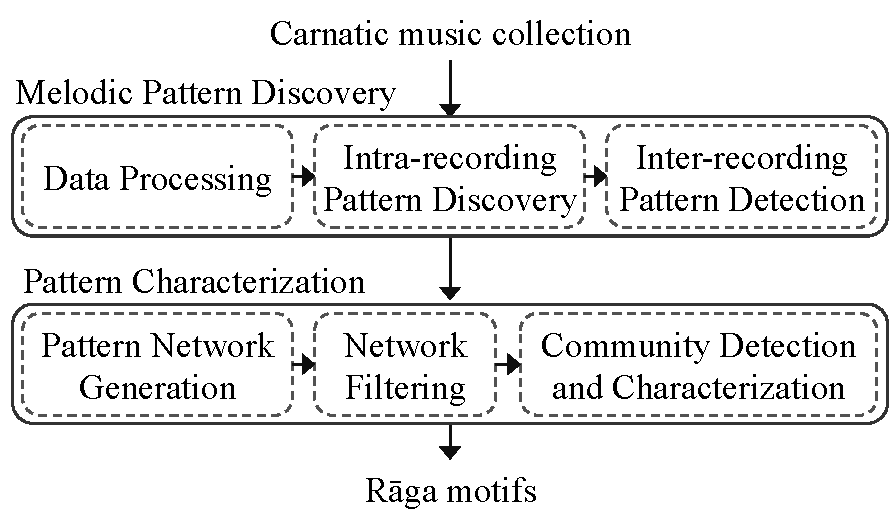
\includegraphics[width=\figSizeSeventy]{ch06_patterns/figures/Characterization/blockDiagram.pdf}
	\end{center}
	\caption[Block diagram for characterizing melodic patterns]{Block diagram of the proposed approach for characterizing melodic patterns.}
	\label{fig:block_diagram_characterization}
\end{figure}


\subsubsection{Melodic Pattern Discovery}
\label{sec:patterns_characterization_pattern_discovery}

As mentioned, discovering melodic patterns in a sizable audio collection of \gls{iam} is a challenging task. To get a reliable input for our approach, we employ the pattern discovery approach we describe in~\secref{sec:patterns_melodic_pattern_discovery}. This is one of the few unsupervised systems, we are aware of, that can discover meaningful melodic patterns in large-scale collections of \gls{iam}. Recall that the output of our pattern discovery approach comprises seed patterns, which are discovered within the recordings, and also, their nearest neighbors in the entire audio collection. In this study, we extract the top 25 closest seed pattern pairs from every recording and consider the top 20 closest patterns for each seed pattern across the recordings. We use the same parameter settings and the implementation of the method as described in~\secref{sec:patterns_melodic_pattern_discovery}. 

Notice that the output of our melodic pattern discovery system may contain a high degree of redundancy in terms of overlapping patterns. This is despite the constraints to only select mutually non-overlapping patterns during the discovery and search phase. This redundancy arises primarily because we perform the inter-recording pattern search for each pattern in the seed pair. Since seed pair patterns are (often) close repetitions of each other, we end up retrieving nearly the same set of patterns as nearest neighbors for both of them. Thus, there exists a large number of overlapping patterns in the output of our pattern discovery block. Despite the known redundancy, we chose to perform inter-recording pattern search for each pattern in the pair separately as it exploits intra-class variability present in the patterns, which might provide better retrieval results.

We reduce the above mentioned redundancy in the output of pattern discovery by following a simple procedure. For every discovered melodic pattern we search for its closest pattern across all the recordings using the same similarity measure as used in the intra-recording pattern discovery block. For each recording we parse a list of patterns in that recording sorted in the increasing order of their distances from their closest patterns. While parsing the list we remove every pattern for which there exists an overlap with another pattern placed higher (lower index) in the sorted list. Thus, at the end of this process we retain only non-overlapping patterns in every recording.



\subsubsection{Melodic Pattern Characterization}
\label{pattern_characterization}

Before we formally describe this processing step, we provide the underlying intuition behind it. As explained earlier, a repeating melodic pattern in \gls{iam} can correspond to either a \gls{raga} motif, a composition-specific motif or to a \gls{gamaka} pattern (\secref{sec:melody_in_iam}). Our objective is to characterize the discovered patterns in order to identify the ones that are \gls{raga} motifs. The information available to accomplish this task is: a bunch of melodic patterns, pitch sequences corresponding to the patterns, editorial metadata of the recordings to which the patterns belongs and the location of the patterns in the recordings. If we take a single melodic pattern, the only possible indicator of its category could be the characteristics of its pitch sequence. However, to the best of our knowledge (acquired from published studies and discussions with musicians), \gls{raga} motifs do not possess any distinctive pitch characteristics. Therefore, characterization of the discovered melodic patterns considering one pattern at a time under unsupervised scenario appears to be virtually impractical. Such melodic motifs are explicitly learned for each \gls{raga} though years of musical training. Despite the importance, a comprehensive published collection of \gls{raga} motifs (audio or pitch sequence) is unavailable. 

Instead of analyzing melodic patterns individually, if we analyse them in clusters, where a cluster comprises melodically similar melodic patterns, we can infer to an extent the categories of these melodic patterns. Consider that we have a cluster of melodic patterns and each pattern comes from a different recording in different \gls{raga}. There is a very high chance that the patterns in the cluster belongs to \gls{gamaka} category, since those patterns occur across \glspl{raga} and across recordings. On the other hand if patterns within a cluster belongs to only one \gls{raga} and different recordings, it is highly likely that the patterns correspond to a \gls{raga} motif. Thus, by analyzing the properties of a cluster in terms of its relation with different musical attributes and editorial metadata, we can characterize the patterns as belonging to \gls{raga} motifs or not. Notice that we eventually exploit the functional roles of different kinds of patterns in melodies of \gls{iam} in order to identify them in a pool of discovered patterns. 

We described above our intuition behind analyzing melodic patterns in units of clusters in order to characterize them. However, clustering melodic patterns further involves many challenges. During clustering we seek to group melodic patterns such that a cluster contains different occurrences of only one melodic phrase. To achieve this, our system should be able to differentiate between melodically similar and dissimilar patterns, for which we need a meaningful similarity threshold. Recall that the extraction of melodic patterns from audio recordings does not involve any similarity thresholding (\secref{sec:patterns_melodic_pattern_discovery}), we select the top 25 and 20 nearest neighbors in discovery and search phase. Determining a musically meaningful similarity threshold in an unsupervised setup is a challenging task, which we address using the concepts of complex networks. 
 
We now formally describe the processing block. As explained, in this block, we aim to first cluster the discovered patterns and then characterize the clusters in order to identify the ones that represent different \gls{raga} motifs. For this, we perform a network analysis in which nodes represent the discovered melodic patterns and edges represent the melodic similarities between these patterns. We described below the processes involved in this task~(\figref{fig:block_diagram_characterization}). 


\paragraph{Pattern Network Generation}
\label{sec:network_generation}

We start by building an undirected weighted network using the discovered melodic patterns from the previous step. The patterns are considered as the nodes of the network and the edge between any two patterns ($i$, $j$) is weighted based on the distance $\distPatt_{ij}$ between the patterns. Noticeably, $\distPatt_{ij}$ is computed using the same distance measure as used in the intra-recording pattern discovery block in~\secref{sec:intraRecordingPatternDiscovery}. The weight of the edge $\edgeWght_{ij}$ between the nodes $i$ and $j$ is given by \eqref{eq:edge_weight_in_network}. 
\begin{equation}
\edgeWght_{ij} = e^{\nicefrac{-\distPatt_{ij}}{\bar{\distPatt}}},
\label{eq:edge_weight_in_network}
\end{equation}
\noindent where, $\bar{\distPatt}$ is the mean of $\distPatt_{ij}$ over every combination of $i$ and $j$. 


\paragraph{Network Filtering}
\label{sec:network_filtering}

The main objective of this processing block is to filter the network in order to retain only the musically meaningful connections between the nodes. Since the edge weights between the pairs of melodically similar and dissimilar nodes may vary by orders of magnitude, we first consider to exploit this heterogeneity to extract the network's backbone. We therefore apply disparity filtering~\citep{Serrano09PNAS} to preserve only the edges that represent statistically significant deviations with respect to a null model of edge weight assignment for every node. The only parameter used in the disparity filtering is the statistical confidence value. We iterate over 5 different confidence values $\lbrace$99.99, 99, 90, 80, 50$\rbrace$. However, as we will show, the application of disparity filtering is found to be quite irrelevant for the present case.

We next proceed to filter edges in the network based on a melodic similarity threshold $\simThsld$. As mentioned, determining a meaningful similarity threshold in an unsupervised setup is a challenging task. We propose to estimate $\simThsld$ based on the topological properties of the network. For this, we analyse the evolution of the clustering coefficient of both the obtained network $\netUndirWght$ and the corresponding randomized network $\netUndirWght_r$ over a range of similarity thresholds. Clustering coefficient measures the extent to which the nodes in a network tend to cluster together~\citep{newman2003structure}. The randomized network $\netUndirWght_r$ is obtained by swapping the edges between randomly selected node pairs such that the degree of each node is preserved~\citep{maslov2002specificity}. This way, $\netUndirWght_r$ can be considered as the maximally random network with that particular degree distribution. In~\figref{fig:cc_curve_pattern_characterization}, we show the evolution of the clustering coefficient of $\netUndirWght$ and $\netUndirWght_r$ over different similarity thresholds (indicated by exponentially spaced bins). In addition, we can also see the clustering coefficient curves for different statistical confidence values used for disparity filtering. The evolution of the clustering coefficients is used for obtaining a similarity threshold as explained below.

\begin{figure}
	\begin{center}
		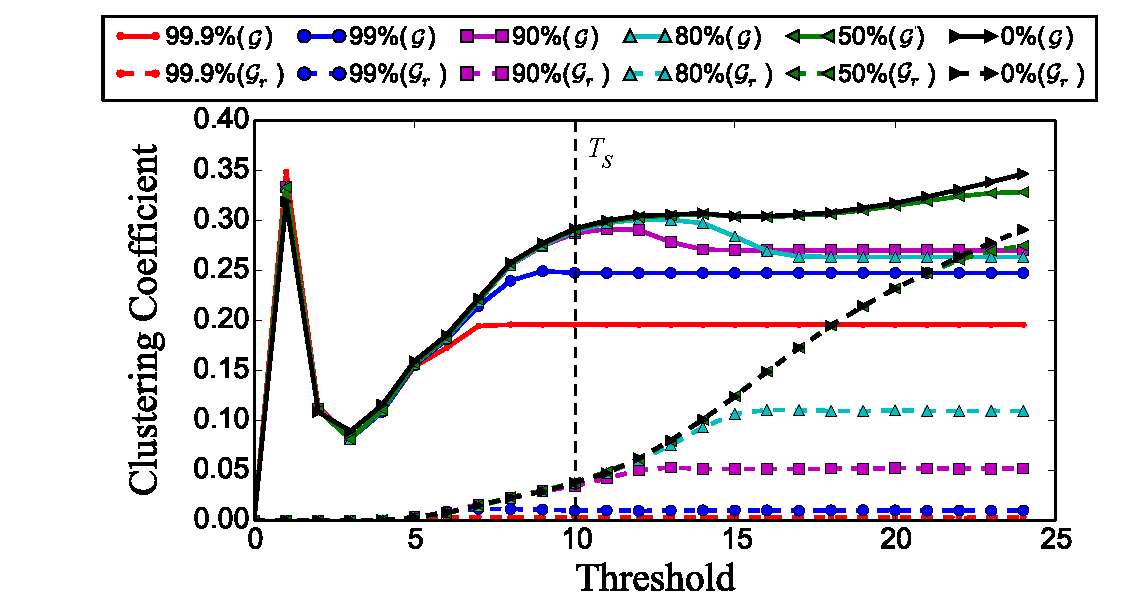
\includegraphics[width=\figSizeNinety]{ch06_patterns/figures/Characterization/CC_Curves_shrunk.pdf}
	\end{center}
	\caption[Evolution of the clustering coefficient of a network of melodic patterns]{Evolution of the clustering coefficient of $\netUndirWght$ and $\netUndirWght_r$ over different thresholds and for different statistical confidence values used for disparity filtering (see legend).}
	\label{fig:cc_curve_pattern_characterization}
\end{figure}

We hypothesize that the more musically meaningful $\simThsld$ is, the higher is the difference between the clustering coefficients of $\netUndirWght$ and $\netUndirWght_r$. We therefore select $\simThsld=10$. Note that even though the similarity threshold corresponding to $\simThsld=1$ results in a higher value of the clustering coefficient, we reject it because the filtered network consists only of a small number of nodes. These nodes correspond to near-exact pattern repetitions discovered within the same recording. Such patterns typically represent composition-specific motifs, and hence are irrelevant in our context. In~\figref{fig:cc_curve_pattern_characterization}, we also observe that the disparity filtering using a confidence value higher than 80\% significantly lowers the clustering coefficient, which can be attributed to the removal of musically meaningful edges in the network. On the other hand, given $\simThsld=10$, the disparity filtering with a confidence value lower than 80\% does not significantly affect the clustering coefficient. We can thus conclude that, in the given scenario, disparity filtering does not bring in any clear advantage. Finally, after applying $\simThsld$, we transform $\netUndirWght$ to an unweighted network. 


\paragraph{Community Detection and Characterization}
\label{sec:patterns_characterization_community_detection}

We next take the unweighted undirected network that results from the previous step, and perform a non-overlapping community detection using the method proposed in~\cite{blondel2008fast}. This method is based on modularity optimization and is parameter-free from the point of view of the user. It has been extensively used in various applications~\citep{fortunato2010community} and can deal with very large networks~\citep{blondel2008fast}. We use the implementation available in networkX~\citep{hagberg-2008-exploring}, a Python language package for exploration and analysis of networks and network algorithms. Using this method for our entire dataset, we obtain around 1800 communities of melodic patterns. 


\begin{figure}
	\begin{center}
		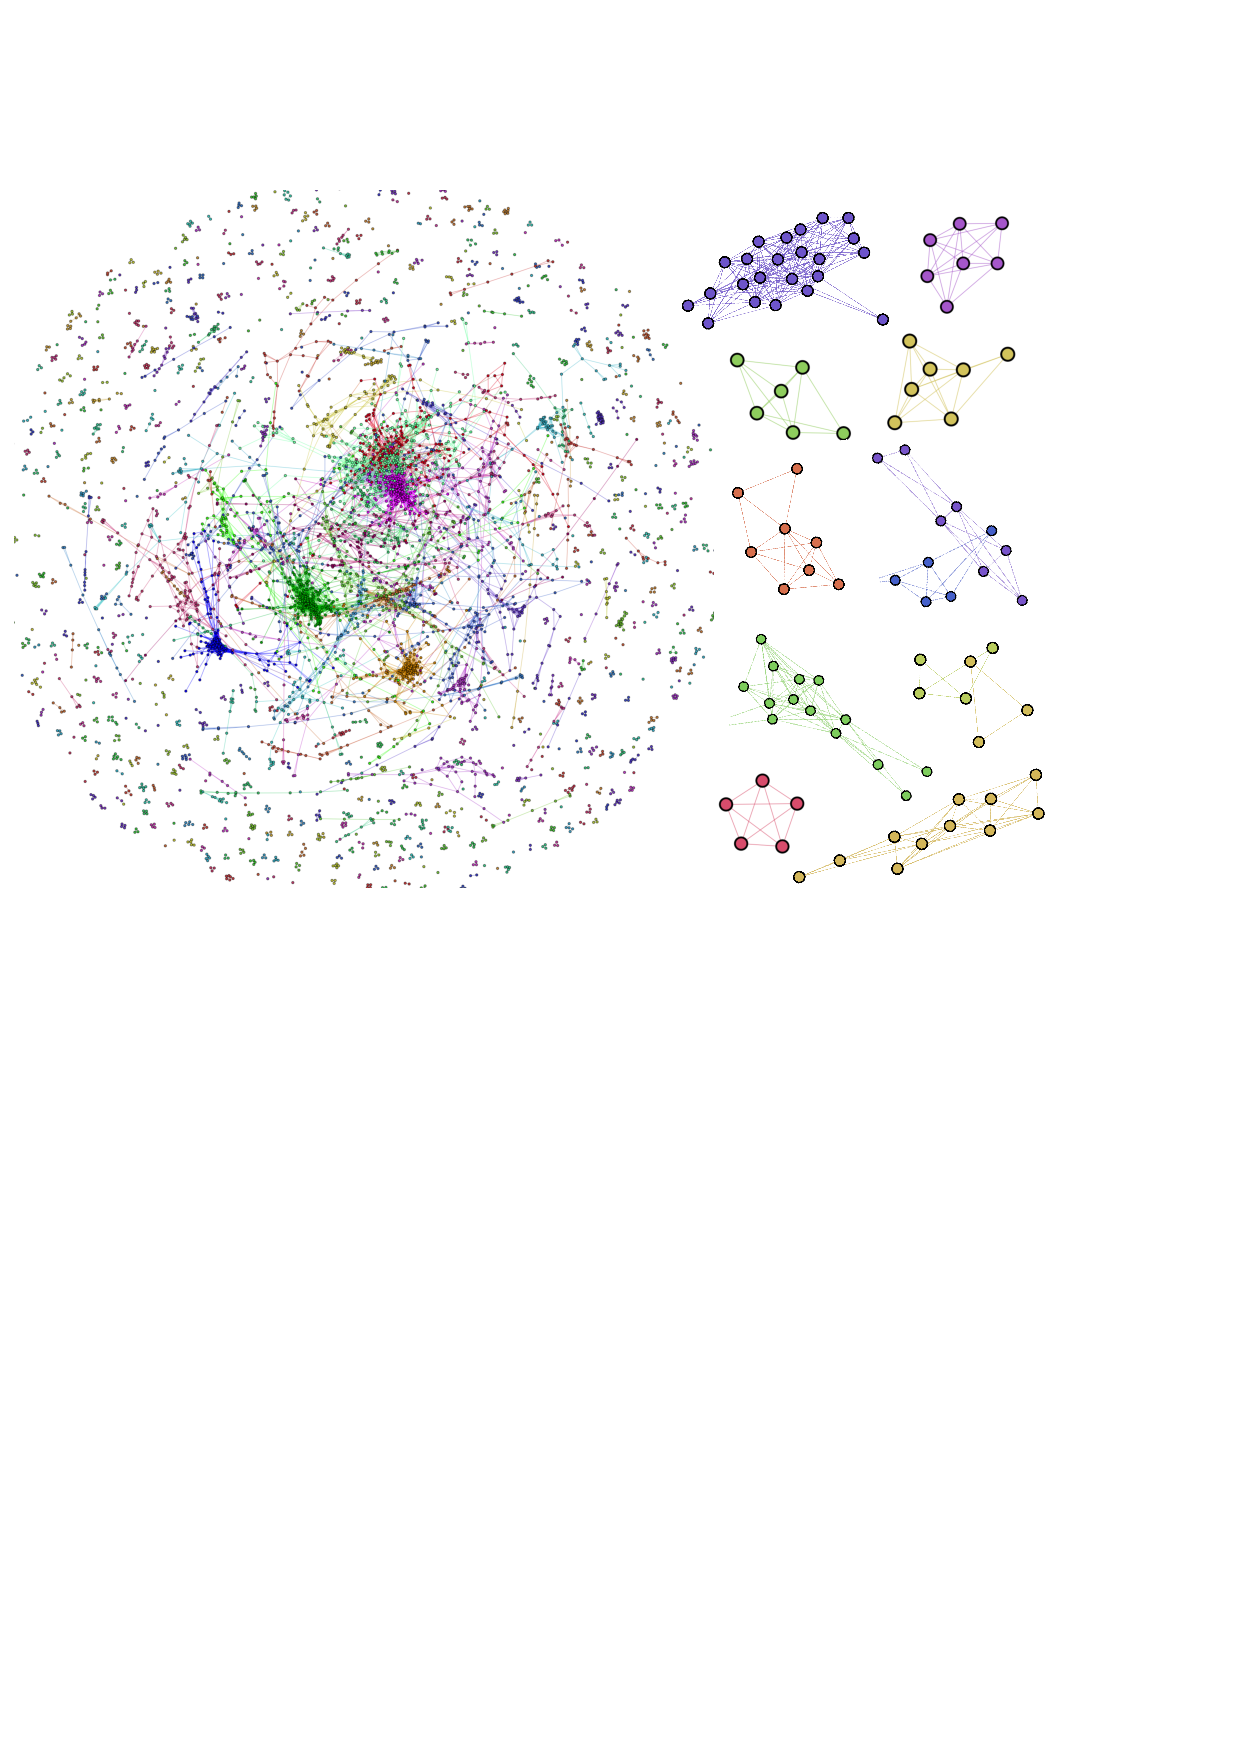
\includegraphics[width=\figSizeHundred]{ch06_patterns/figures/Characterization/networkWithClusters.pdf}
	\end{center}
 \caption[Graphical representation of a network of melodic patterns]{Graphical representation of the melodic pattern network after filtering by threshold $\simThsld$. The detected communities in the network are indicated by different colors. Few examples of these communities are shown on the right.}
 \label{fig:network_and_communities_pattern_characterization}
\end{figure}

To get a better understanding of the network obtained after filtering and the detected communities, we show a graphical representation of the network in~\figref{fig:network_and_communities_pattern_characterization}. We find that many communities comprising large number of nodes in the network correspond to \gls{kampitam} melodic pattern, which is a kind of \gls{gamaka} that occur in several \glspl{raga} across compositions and hence have large number of occurrences. We also find that the communities with a relatively smaller number of nodes, which in~\figref{fig:network_and_communities_pattern_characterization} appear as isolated communities around the periphery often correspond to the \gls{raga} motifs. A few examples of such communities are shown in~\figref{fig:network_and_communities_pattern_characterization} on the right.

We here define the notation used in the subsequent paragraphs for characterizing pattern communities. A community $\community_q$ is comprised of $N$ nodes, and the node count over different \glspl{raga} is given by the ordered list ${{\nodesCommRaga}_q} = (\nodesCommRaga_{q,1}, \nodesCommRaga_{q,2},\dots$ $\nodesCommRaga_{q,\totalRagasComm})$ such that $\nodesCommRaga_{q,i} \geq \nodesCommRaga_{q,j}$, $\forall~ i < j$,
where each element in $\nodesCommRaga_{q}$ denotes the number of nodes in a particular \gls{raga} and $\totalRagasComm$ is the total number of unique \glspl{raga} comprising the community. Similarly, the node count over the audio recordings is given by the ordered list ${{\nodesCommRec}_q} = (\nodesCommRec_{q,1}, \nodesCommRec_{q,2},\cdots,\nodesCommRec_{q,\totalRecsComm})$ such that $\nodesCommRec_{q,l} \geq \nodesCommRec_{q,m}, \forall~l < m$, where each element in $\nodesCommRec_{q}$ denotes the number of nodes belonging a particular audio recording and $\totalRecsComm$ is the total number of recordings comprising the community. For both these cases, $\sum_{i=1}^{\totalRagasComm}\nodesCommRaga_{q,i} = \sum_{l=1}^{\totalRecsComm}\nodesCommRec_{q,l} = N$.

We now proceed to characterize the detected communities in order to identify the ones that represent \gls{raga} motifs. For that we first categorize a community $C_q$ as belonging to the \gls{raga} $\RagaOfComm_q$ corresponding to the maximum number of nodes $\nodesCommRaga_{q,1}$ in that community. Subsequently, for each \gls{raga}, we rank all the communities belonging to that \gls{raga}. To rank the communities we empirically devise a goodness measure $\goodnessComm$, which denotes the likelihood that a community $C_q$ represents a \gls{raga} motif. We propose to use

\begin{equation}
\goodnessComm = N \ragaLikelihood^4 \recDistCentroid,
\label{eq:gamma_pattern_characterization}
\end{equation}

where $\ragaLikelihood$ is an estimate of the likelihood of \gls{raga} $\RagaOfComm_q$ in $C_q$, 

\begin{equation}
\ragaLikelihood = \frac{\nodesCommRaga_{q,1}}{N},
\end{equation}

and $\recDistCentroid$ indicates how uniformly the nodes of the community are distributed over audio recordings,

\begin{equation}
\recDistCentroid = \frac{\sum_{l=1}^{\totalRecsComm}l \cdot \nodesCommRec_{q,l}}{N}.
\end{equation}

Higher $\recDistCentroid$ implies a more uniform distribution. Since a community that represents a \gls{raga} motif is expected to contain nodes from a single \gls{raga} (high value of $\ragaLikelihood$) and the nodes belong to many different recordings (high value of $\recDistCentroid$), the goodness measure $\goodnessComm$ is high for such a community. In general we prefer large communities, but, to avoid detecting large communities (high value of N) corresponding to \gls{gamaka} motifs (low value of $\ragaLikelihood$) we use a fourth power on $\ragaLikelihood$. Composition-specific motifs are expected to have a low $\recDistCentroid$, as they are not repeated across multiple recordings, assuming that different recordings correspond to different compositions. 

Note that it might be possible that a music collection contains multiple recordings of the same composition. In such cases, differentiating composition-specific motifs and \gls{raga} motif becomes difficult using $\goodnessComm$ measure. This issue can be overcome with only a trivial modification in our approach, i.e.,~by considering the node distribution ${{\nodesCommRec}_q}$ over compositions instead of recordings. In our current system this could not be implemented because for a number of recordings composition information was unavailable.



\subsection{Evaluation}
\label{sec:patterns_characterization_evaluation}

\subsubsection{Music Collection}
\label{sec:patterns_characterization_music_collection}

The music collection used in this study is a subset of the CompMusic Carnatic music corpus (\secref{sec:corpus_carnatic_music_corpus}). The collection comprises 44 hours of polyphonic audio music recordings of Carnatic music across 10 different \glspl{raga}. For each \gls{raga} we select 16 music pieces, which amounts to a total of 160 recordings. There are 139 vocal music recordings and 21 instrumental recordings comprising violin, \gls{vina} and bamboo flute. In~\tabref{tab:dataset_details_pattern_characterization}, we summarize the relevant details of the dataset. We see that it is diverse in terms of the number of unique compositions and number of lead artists. Furthermore, it includes different forms of compositions (\gls{kirtana}, varnam and viruttam) and recordings containing varied improvised sections such as \gls{alapna}, nereval and kalpan\={a}-\glspl{svara}. %The \glspl{raga} selected here are amongst the most frequently performed \glspl{raga} in the CompMusic Carnatic music corpus, which in turn is representative of the Carnatic music repertoire~\cite{CM_Corpora_Ajay14}. 
The chosen \glspl{raga} contain diverse set of \glspl{svara} (notes) both in terms of the number of \glspl{svara} and their pitch classes (svarasth\={a}n\={a}s). From~\tabref{tab:dataset_details_pattern_characterization}, 
we also notice that several \glspl{raga} such as Kaly\={a}\d{n}i, K\={a}mb\={o}ji and B\={e}gada have a large fraction of \glspl{svara} in common. We refer to them as allied \glspl{raga} (\secref{sec:melody_in_iam}). This further increases the complexity of the task at hand, since the discrimination between the phrases of allied \glspl{raga} may be based on subtle melodic nuances.

\begin{table} 
	%\tabcolsep = 0.1cm
	\centering
	\begin{tabular}{ l  | c c c c}
\tabletop
		\Gls{raga}   		& 	Dur 	&	\#Com		&	\#Art	&	\Glspl{svara}\\	
\tablemid
		Hamsadhvani 		& 	2.46 		&	12			&	14		&	$s\,r_2\,g_3\,p\,n_3$\\
		K\={a}mavardhini 	& 	3.94 		&	13			&	16		&	$s\,r_1\,g_3\,m_2\,p\,d_1\,n_3$\\		
		Darb\={a}r   		& 	2.59 		&	8			&	13		&	$s\,r_2\,g_2\,m_1\,p\,d_2\,n_2$\\	
		Kaly\={a}\d{n}i   	& 	6.94 		&	9			&	16		&	$s\,r_2\,g_3\,m_2\,p\,d_2\,n_3$\\	
		K\={a}mb\={o}ji   	& 	6.91 		&	12			&	13		&	$s\,r_2\,g_3\,m_1\,p\,d_2\,n_2\,n_3$\\	
		B\={e}ga\d{d}a   	& 	3.41 		&	9			&	16		&	$s\,r_2\,g_3\,m_1\,p\,d_2\,n_2\,n_3$\\	
		K\={a}pi   			& 	2.24 		&	12			&	16		&	$s\,r_2\,g_2\,g_3\,m_1\,p\,d_2\,n_2\,n_3$\\	
		Bhairavi   			& 	5.33 		&	7			&	16		&	$s\,r_2\,g_2\,m_1\,p\,d_2\,d_3\,n_2$\\	
		Beh\={a}g   		& 	1.51 		&	12			&	16		&	$s\,r_2\,g_3\,m_1\,m_2\,p\,d_2\,n_2\,n_3$\\	
		
		T\={o}\d{d}i   		& 	8.75 		&	12			&	16		&	$s\,r_1\,g_2\,m_1\,p\,d_1\,n_2$\\	
\tablebot
		Total 	& 	44.08 		&	106			&	57		&	-\\	
\tablebot
	\end{tabular}
	\caption[Details of the dataset used for studying pattern characterization]{Details of the dataset in terms of the duration (Dur) in hours, number of unique compositions (\#Com), unique lead artists (\#Art), and the \glspl{svara} for each \gls{raga}. Here $s,r,$ $g,m,p,d,n$ denote the seven \glspl{svara} in \gls{iam} and the subscript indicates the variant of the \gls{svara} for a particular \gls{raga} (cf.~\citep{Viswanathan2004}).\TODO{Remove svaras and say its explained in Table XX.}}
	\label{tab:dataset_details_pattern_characterization}
\end{table}

\subsubsection{Setup and Evaluation Measures}
\label{sec:patterns_characterization_experimental_setup}

Given the unsupervised nature of this study, we perform a listening test to formally evaluate the extent to which the selected melodic phrases correspond to \gls{raga} motifs. For each of the 10 \glspl{raga} in the dataset, we select the top 10 communities based on the goodness measure $\goodnessComm$ (\eqnref{eq:gamma_pattern_characterization}). From each of these communities, we select their representative melodic phrase based on the betweenness centrality of the nodes~\citep{newman2003structure}, i.e.,~the node with the highest betweenness centrality is considered as the representative melodic phrase of that community. In case of a tie, we select the one with the highest node degree~\citep{newman2003structure}. Finally, we arrive at a set of 100 melodic phrases, which are then used to perform the listening test. These audio examples are also made available online (see the companion page of the corresponding study in~\appref{app:mypapers}).

For the listening test we select 10 professional Carnatic musicians with over 15 years of formal music training. Each musician is presented with the audio fragments corresponding to the selected melodic phrases in a random order. They are also presented with the \glspl{raga} corresponding to the melodic phrases. The musicians are asked to rate each melodic phrase based on whether it is a characteristic phrase of that \gls{raga}. We use binary ratings (`Yes' or `No'). 

The audio fragments were segmented with a one second buffer on either side of the phrase to offer some context and reduce the effect of abrupt boundaries. % Thus, a 4\,s audio fragment was presented to the musicians.  
In order to quantify the musicians' assessment, we use mean ratings for each phrase $\pattern$, $\mu_\pattern$, considering `Yes' as 1 and `No' as 0. For analyzing the ratings per \gls{raga}, we study the mean and standard deviation of all $\mu_\pattern$ for phrases in every \gls{raga}, which we denote by $\mu_\recording$ and $\sigma_\recording$, respectively.


\subsection{Results and Discussion}
\label{sec:patterns_characterization_results_and_discussion}

We first analyse the musicians' ratings at the level of melodic phrases. In~\figref{fig:average_rating_pattern_characterization}, we show $\mu_\pattern$ for the 100 selected melodic phrases, where the grouping is based on their corresponding \glspl{raga}. We find that the mean and the standard deviation of $\mu_\pattern$ for the melodic phrases is 0.85 and 0.16, respectively. For a better understanding of $\mu_\pattern$ across phrases and the overall musicians' agreement, we show the histogram of $\mu_\pattern$ in~\figref{fig:average_rating_histogram_pattern_characterization}. We see that 33 melodic phrases are rated as \gls{raga} motifs by all 10 musicians and 25 phrases are rated as \gls{raga} motifs by 9 out of 10 musicians. Similarly, the musicians' agreement can be inferred for the rest of the phrases from this histogram. We observe that 91\% of the phrases are always marked as \gls{raga} motifs by at least 7 out of 10 musicians. 


\begin{figure}
	\begin{center}
		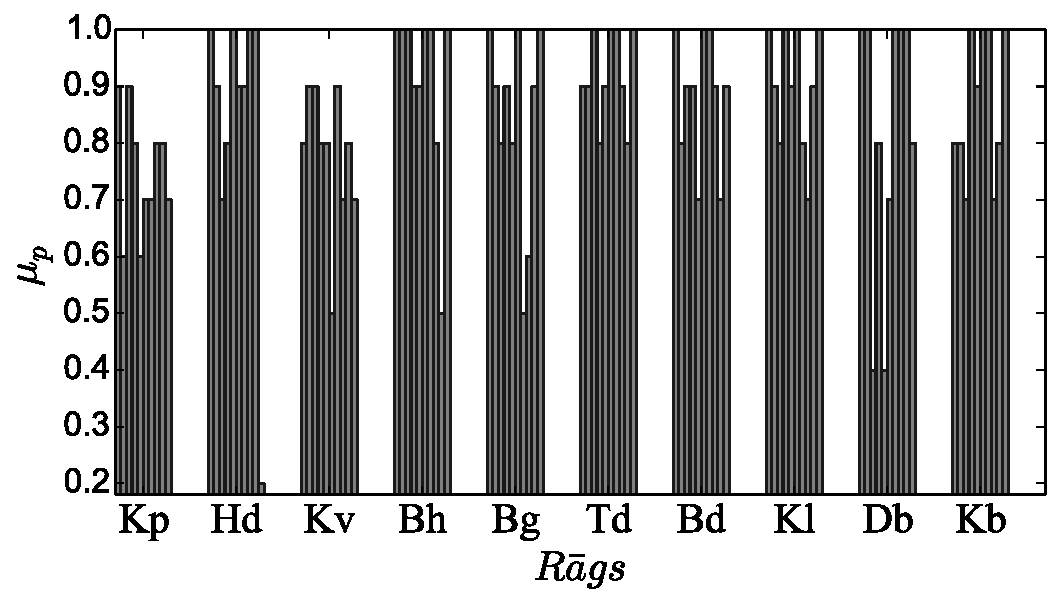
\includegraphics[width=\figSizeEighty]{ch06_patterns/figures/Characterization/per_raaga_per_phrase_rating.pdf}
	\end{center}
	\caption[Mean musician ratings for the discovered melodic phrases]{Mean musician rating per melodic phrase for each \gls{raga}: K\={a}pi\,(Kp), Hamsadhvani\,(Hd), K\={a}mavardhini\,(Kv), Bhairavi\,(Bh), Beh\={a}g\,(Bg), T\={o}\d{d}i\,(Td), B\={e}ga\d{d}\={a}\,(Bd), Kaly\={a}\d{n}\={i}\,(Kl), Darb\={a}r\,(Db), K\={a}mb\={o}ji\,(Kb).}
	\label{fig:average_rating_pattern_characterization}
\end{figure}


We now proceed to analyse the results for different \glspl{raga}. In~\tabref{tab:results_per_raaga_pattern_characterization}, we summarize mean $\mu_\recording$ and standard deviation $\sigma_\recording$ of $\mu_\pattern$ for each \gls{raga}. We observe that there is a considerable amount of variation in $\mu_\recording$ across the \glspl{raga}. It ranges from 0.75 for \gls{raga} K\={a}pi to 0.92 in the case of \gls{raga} T\={o}\d{d}i. An interesting observation here is that the phrase-based \glspl{raga}\footnote{\Glspl{raga} whose identity is primarily derived based on phraseology than the \glspl{svara}~\citep{krishna2012carnatic}} are the top performing \glspl{raga} with the exception of \gls{raga} Darb\={a}r. From~\tabref{tab:results_per_raaga_pattern_characterization} and \tabref{tab:dataset_details_pattern_characterization}, we notice a strong correlation between $\mu_\recording$ and the total duration of the audio recordings across \glspl{raga}. This suggests that longer music pieces are likely to facilitate the discovery of \gls{raga} motifs owing to more number of occurrences of such melodic phrases.

\begin{table} 
	%\tabcolsep = 0.1cm
	\centering
	\begin{tabular}{ l  c c| l | c c }
		\hline\hline
		\multicolumn{1}{ l|  }{\Gls{raga}}   			& 	$\mu_\recording$ 	&	$\sigma_\recording$	& \Gls{raga}   			& 	$\mu_\recording$ 	&	$\sigma_\recording$\\	
		\hline
		\multicolumn{1}{ l|  }{Hamsadhvani} 			& 	0.84 		&	0.23 & {\bf B\={e}ga\d{d}a}   	& 	0.88 		&	0.11	\\
		\multicolumn{1}{ l|  }{K\={a}mavardhini} 	& 	0.78 		&	0.17 & K\={a}pi   			& 	0.75 		&	0.10\\	
		\multicolumn{1}{ l|  }{Darb\={a}r}   		& 	0.81 		&	0.23 & {\bf Bhairavi}   			& 	0.91 		&	0.15\\	
		\multicolumn{1}{ l|  }{\bf Kaly\={a}\d{n}i}  & 	0.90 		&	0.10 & Beh\={a}g   		& 	0.84 		&	0.16\\	
		\multicolumn{1}{ l|  }{\bf K\={a}mb\={o}ji}   	& 	0.87 	&	0.12 & {\bf T\={o}\d{d}i}   		& 	0.92 		&	0.07\\	
		\hline\hline
		%   			& 				& 		& 	Overall&0.85 		&	0.16\\ \cline{4-6}\cline{4-6}
		%\hline\hline 
	\end{tabular}
	\caption[Mean and standard deviation of $\mu_\pattern$ for each \gls{raga}]{Mean ($\mu_\recording$) and standard deviation ($\sigma_\recording$) of $\mu_\pattern$ for each \gls{raga}. R\={a}gas with $\mu_\recording \geq 0.85$ are highlighted. }
	\label{tab:results_per_raaga_pattern_characterization}
\end{table}
\begin{figure}
	\begin{center}
		\ifdefined\PRINTVER
			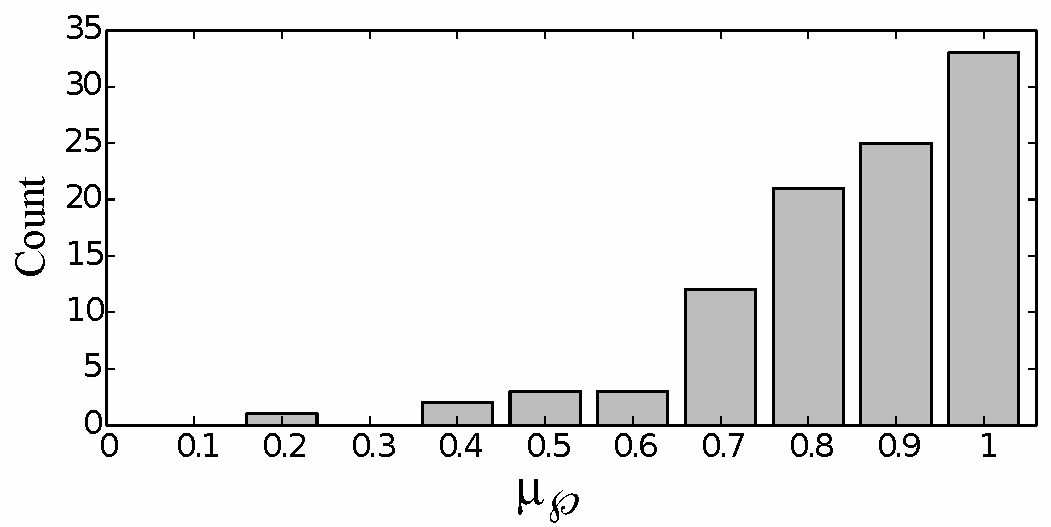
\includegraphics[width=\figSizeSeventy]{ch06_patterns/figures/Characterization/histogram_musician_rating_BW.pdf}
		\else
			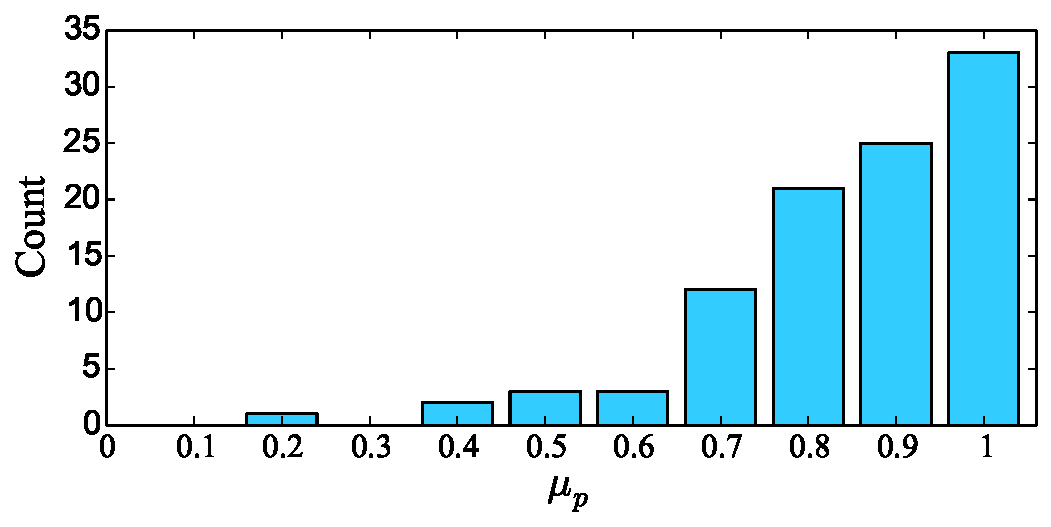
\includegraphics[width=\figSizeSeventy]{ch06_patterns/figures/Characterization/histogram_musician_rating.pdf}
		\fi
	\end{center}
	\caption[Histogram of mean musician ratings for all of the 100 melodic phrases]{Histogram of $\mu_\pattern$ for all of the 100 melodic phrases selected for the listening test.}
	\label{fig:average_rating_histogram_pattern_characterization}
\end{figure}



We examine the melodic phrases with low scores. An investigation of 9 out of 100 phrases that obtain $\mu_\pattern\leq0.6$ reveals that many of these phrases are composition-specific phrases that do not characterize the \gls{raga}. The method wrongly identifies them as \gls{raga} motifs because their associated communities have a high $\goodnessComm$ score owing to a high $\recDistCentroid$ value. This can be attributed to the fact that these phrases are discovered from multiple recordings, since their corresponding compositions have several recordings in the dataset. As described in~\secref{sec:patterns_characterization_community_detection}, in such a scenario, the goodness measure $\goodnessComm$ can be made more robust to such cases by computing $\recDistCentroid$ using the distribution of nodes ${{\nodesCommRec}_q}$ over unique compositions rather than over audio recordings.

The results show that the proposed method successfully discovers \gls{raga} motifs with a high accuracy. We see that, even for the allied \glspl{raga} present in the dataset such as K\={a}mb\={o}ji and B\={e}gada (\secref{sec:patterns_characterization_music_collection}), the method is able to discover distinct characteristic \gls{raga} motifs. As mentioned, allied \glspl{raga} are challenging because they have a substantial overlap in the set of \glspl{svara} that they comprise (see also~\tabref{tab:dataset_details_pattern_characterization}). Finally, on a more informal side, it is worth mentioning that musicians were impressed when, after the listening test, they came to know that the melodic phrases were discovered by a machine following an unsupervised approach. 





We consider this work as a preliminary study with a lot of scope for improvements. In particular, the approach can be extended to identify patterns belonging to other categories (\gls{gamaka} or composition-specific patterns), definition of the goodness measure $\goodnessComm$ can be improved as suggested in~\secref{sec:patterns_characterization_results_and_discussion}, listening test could be done more rigorously by including negative examples (\gls{gamaka} patterns), and the resultant patterns of the approach can be quantitatively evaluated by using them in tasks such as composition identification. On these lines, in~\secref{sec:pattern_based_raga_recognition} we present an approach that uses clustered melodic patterns to perform the task of automatic \gls{raga} recognition. That way, in addition to the qualitative assessment as done in this work, we can also quantitatively assess the musical relevance of the extracted and characterized melodic patterns.



\section{Summary and Conclusions}
\label{sec:conclusions_patterns}

In this chapter we presented our methodology for discovering musically significant melodic patterns in sizable audio music collections of \gls{iam}. Our methods utilize the melodic representations and descriptors obtained in~\chapref{chap:data_preprocessing}, and combine concepts from music signal processing, time-series analysis, information retrieval, and complex networks to successfully extract musically meaningful melodic patterns in audio collections. We studied three main tasks involved in this process: melodic similarity, pattern discovery, and characterization of the discovered melodic patterns. 

We first carried out an in-depth supervised analysis of melodic similarity, which is a crucial component in pattern discovery. We evaluated 560 different combinations of various computational procedures and parameters values that are often used for this task. We showed that melodic similarity computation is very sensitive to the choice of parameters and processing steps. A higher sampling rate of the melody representation and mean normalization is desired for computing a reliable melodic similarity in Carnatic music. For Hindustani music, on the other hand, sampling rate (within the considered range) has no significant affect on the performance and tonic normalization of the melody results in a better performance. In general, \gls{dtw}-based distance measure performs better than the Euclidean distance, and the usage of local constraint in \gls{dtw} enhances the performance. The \gls{dtw} variant without any global constraint is preferred (specially for Hindustani music), which suggests that there are large non-linear timing variations across occurrences of the melodic pattern. We observed that an accurate segmentation of the melodic patterns has a huge positive impact on the computation of melodic similarity. The best methodology variant thus identified for melodic similarity is further improved by addressing two specific challenges that arise due to large non-linear timing variations and rapid melodic movements in melodic patterns. The solution we proposed exploits specific melodic characteristics that are particular to \gls{iam}. We showed that duration truncation of the steady \gls{svara} regions in melodic phrases results in a statistically significant improvement in the computation of melodic similarity. Furthermore, we showed that the complexity of a melodic pattern in Carnatic music is a distinguishing aspect of the pattern, and can be successfully utilized to improve melodic similarity.

Subsequently, we presented our data-driven unsupervised approach for discovering repeated melodic patterns in large audio collections of \gls{iam}. We first discovered seed patterns within a recording, and later, used those as queries to detect similar occurrences in the entire music collection. We used \gls{dtw}-based distance measures to compute melodic similarity and compared four different rank refinement variants. Discovering 25 closest seed pattern pairs within each recording and retrieving their 200 closest patterns in an audio collection of 365\,hours of Carnatic music comprising 1764 recordings results in around 12 trillion distance computations. We showed that using cascaded lower bounding techniques borrowed from time-series analysis we save nearly 76\% of the total computations for the intra-recording pattern discovery task and around 99\% of the total computations for the inter-recording pattern detection task. Thus, such indexing techniques can scale \gls{dtw} on hundreds of hours of music collections. We evaluated a randomly sampled subset of the extracted melodic patterns comprising 8000 patterns by performing listening tests by a professional Carnatic musician. Our quantitative evaluation based on the expert feedback indicated that a \gls{dtw}-based distance measure performs well for intra-recording discovery. However, the performance for the inter-recording pattern detection task is inferior suggesting that we require better melodic similarity measures for searching occurrences across recordings. Qualitative feedback from the musician suggests that the extracted melodic patterns are interesting and contain several instances of musically significant patterns such as \gls{raga} motifs. 

The output of the pattern discovery method contains different types of repeating patterns. We presented an approach to identify musically significant patterns, the \gls{raga} motifs, and specifically, to distinguish them from \gls{gamaka} and composition-specific patterns (\secref{sec:melody_in_iam}). We employed a network analysis and use a non-overlapping community detection algorithm to cluster melodic patterns. Using the topological properties of the network, we determined a musically meaningful similarity threshold. We devised a goodness measure for characterizing the detected communities. In a listening test with 10 professional Carnatic musicians we showed that the proposed method successfully discovers \gls{raga} motifs with accuracy, even in the presence of allied \glspl{raga} in the dataset. Thus, we demonstrated that the methodology we use to determine melodic similarity threshold and to define the goodness measure successfully identifies musically significant patterns. Our results show that the functional roles of different melodic phrases in \gls{iam} can be effectively exploited to identify them in an unsupervised manner. To the best of our knowledge, utilization of the functional roles of different melodic patterns in \gls{iam} in order to describe and characterize them is done for the first time.

Overall, we showed that our unsupervised methodology that does not require any exemplar patterns can successfully discover musically significant melodic patterns (\gls{raga} motifs) in sizable music collections of \gls{iam}. These patterns can be used in a number of \gls{mir} tasks and applications for \gls{iam}. Due to their importance in characterizing \glspl{raga} they can immediately be utilized for automatic \gls{raga} recognition, a topic that we study in~\chapref{chap:raga_recognition}. These patterns can be used to interlink large volumes of audio recordings in order to define novel music similarity measures, and to perform musicologically relevant studies such as characterization of \glspl{raga}, artists, and compositions in \gls{iam}. Furthermore, there can be enhanced listening music applications, and pedagogical tools that can potentially utilize these melodic patterns. Concrete examples of such applications are provided in~\chapref{chap:applicatoins}.


%FUTURE WORK
%
%It would also be worthwhile to explore the applicability of this approach to music traditions such as Flamenco, Beijing opera and Turkish Makam music.
%
% In the future, we plan to improve the method used for segmenting the steady \gls{svara} regions so that it can differentiate melodic ornaments from subtle \gls{svara} transitions. In addition, we see a vast scope in further refining the complexity estimate of a melodic phrase to improve the complexity weighting. 
% using composition info in communities can further boost the performance of our characterization process. 
